%!TEX TS-program = pdflatex
% dissertation.tex -- main dissertation file
%
% Wisconsin dissertation template
% Copyright (c) 2008-2009 William C. Benton.  All rights reserved.
%
% This program can redistributed and/or modified under the terms
% of the LaTeX Project Public License Distributed from CTAN
% archives in directory macros/latex/base/lppl.txt; either
% version 1 of the License, or (at your option) any later version.
%
% This program includes other software that is licensed under the
% terms of the LPPL and the Perl Artistic License; see README for details.
%
% You, the user, still hold the copyright to any document you produce
% with this software (like your dissertation).
%

%%% You'll want ``oneside'' for the deposit version, but probably not for any versions that don't need to meet the UW requirements
\documentclass[12pt,oneside,letterpaper]{memoir}

% preamble.tex -- packages to include
%
% Wisconsin dissertation template
% Copyright (c) 2008 William C. Benton.  All rights reserved.
%
% This program can redistributed and/or modified under the terms
% of the LaTeX Project Public License Distributed from CTAN
% archives in directory macros/latex/base/lppl.txt; either
% version 1 of the License, or (at your option) any later version.
%
% This program includes other software that is licensed under the
% terms of the LPPL and the Perl Artistic License; see README for details.
%
% You, the user, still hold the copyright to any document you produce
% with this software (like your dissertation).

%% You should use natbib
\IfFileExists{natbib.sty}{%
\usepackage{natbib}%
}{}

%% You probably need appendix, if you want appendices
\IfFileExists{appendix.sty}{%
\usepackage{appendix}%
}{}

%% the spacing in memoir is weird, you'll need to use this
\DisemulatePackage{setspace}
\usepackage[onehalfspacing]{setspace}

%% geometry package to help with margins on title page
\usepackage{geometry}

%% List setup; the ``hanglist`` environment will allow you to have
%% nicely-typeset enumerated lists (i.e. with the numbers hanging in
%% the margins).  You need at least version 2.1 of enumitem.sty.  If
%% you don't have enumitem installed at all, hanglist will just be an
%% alias for enumerate.
\IfFileExists{enumitem.sty}{%
\usepackage[loadonly]{enumitem}[2007/06/30]%
\newlist{hanglist}{enumerate}{1}% 
\setlist[hanglist]{label=\arabic*.}%
\setlist[hanglist,1]{leftmargin=0pt}%
}{%
\newenvironment{hanglist}{\begin{enumerate}}{\end{enumerate}}%
}

%% Comment out any of these that you don't want
\usepackage{amssymb}
\usepackage{amsmath}
\usepackage{amsthm}
%\usepackage{theorem}
\usepackage{hyperref}

\IfFileExists{mathpartir.sty}{%
\usepackage{mathpartir}%
}{}

%%%%% LISTINGS package and setup
\IfFileExists{listings.sty}{%
\usepackage{listings}%
}{}



%% Get rid of ugly borders around PDF hyperlinks (e.g. for cross-references, bib entries, or URLs)
\hypersetup{pdfborder = 0 0 0}

%% You want microtype.
\IfFileExists{microtype.sty}{%
\usepackage[protrusion=true,expansion=true]{microtype}%
}{}

%\pagestyle{thesisdraft}

% Surround parts of graphics with box
\usepackage{boxedminipage}

%% booktabs (thx to Nate Rosenblum for bringing this beautiful package
%% to my attention)
\IfFileExists{booktabs.sty}{%
\usepackage{booktabs}%
}{}

% This is now the recommended way for checking for PDFLaTeX:
\usepackage{ifpdf}

%% Avoid ugly "Type 3" fonts
\usepackage{lmodern}
\usepackage[LY1]{fontenc}

%% Substitute your favorite serif and sans fonts here....
\IfFileExists{tgpagella.sty}{%
% TeX Gyre pagella, like Palatino
\usepackage{tgpagella}%
}{}

\usepackage[LY1]{eulervm}

\ifpdf
\usepackage[pdftex]{graphicx}
\else
\usepackage{graphicx}
\fi

\usepackage{makeidx}
\makeindex

{\theoremstyle{plain}
\newtheorem{thm}{Theorem}[chapter]
\newtheorem{cor}[thm]{Corollary}
\newtheorem{define}[thm]{Definition}
\newtheorem{exmpl}[thm]{Example}
}
{\theoremstyle{remark}
\newtheorem{rmk}[thm]{Remark}
}

\newtheoremstyle{customsty1}
{3pt}%
{3pt}%
{}% --- body font
{}% --- indent amount
{\bfseries}% --- Theorem head font
{:}% --- Punctuation after head
{.5em}% --- space after head
{}% --- theorem head spec (can be left empty, meaning 'normal')

% Define 'newtheorems' that use ``customsty1''
{\theoremstyle{customsty1} 
}


%%% NB: the ``deposit'' chapter- and page- styles should conform to UW
%%% requirements.  If you are producing a pretty version of your
%%% dissertation for web use later, you will certainly want to make
%%% your own chapter and page styles.

\makechapterstyle{deposit}{%
  \renewcommand{\chapterheadstart}{}
  \renewcommand{\printchaptername}{}
  \renewcommand{\chapternamenum}{}
  \renewcommand{\printchapternum}{\parbox{2em}{\MakeLowercase{\Large\scshape\thechapter{}}} }
  \renewcommand{\afterchapternum}{}
  \renewcommand{\printchaptertitle}[1]{%
  \raggedright\Large\scshape\MakeLowercase{##1}}
  \renewcommand{\afterchaptertitle}{%
  \vskip\onelineskip \hrule\vskip\onelineskip}
}

\makepagestyle{deposit}
 
\makeatletter
 
\renewcommand{\chaptermark}[1]{\markboth{#1}{}}
\renewcommand{\sectionmark}[1]{\markboth{#1}{}}
 
\makeevenfoot{deposit}{}{}{}
\makeoddfoot{deposit}{}{}{}
\makeevenhead{deposit}{\thepage}{}{}
\makeoddhead{deposit}{}{}{\thepage}
\makeatother

%%% set up page numbering for chapter pages to satisfy UW requirements
%%% NB: You will want to delete until the ``SNIP'' mark if you are
%%% making a ``nice'' copy
\copypagestyle{chapter}{plain}
\makeoddfoot{chapter}{}{}{}
\makeevenhead{chapter}{\thepage}{}{}
\makeoddhead{chapter}{}{}{\thepage}
%%% SNIP

%%% bib nonsense
\makeatletter
\newenvironment{wb-bib}[1]{%
  \chapter*{references}
\ifnobibintoc\else 
\phantomsection 
\addcontentsline{toc}{chapter}{References} 
\fi 
\prebibhook
  \begin{bibitemlist}{#1}}{\end{bibitemlist}\postbibhook}

\AtBeginDocument{%
  \@ifpackageloaded{natbib}{% natbib is loaded
    \addtodef{\endthebibliography}{}{\vskip-\lastskip\postbibhook}
    \@ifpackagewith{natbib}{sectionbib}{% with sectionbib option
      \renewcommand{\bibsection}{\@memb@bsec}}%
      {\renewcommand{\bibsection}{\@memb@bchap}}}%
  {}
  \@ifpackagewith{chapterbib}{sectionbib}{%
    \renewcommand{\sectionbib}[2]{}
    \renewcommand{\bibsection}{\@memb@bsec}}{}
}
\makeatother

% defs.tex -- wbepi environment for chapter epigraphs and other useful defs.
%
% Wisconsin dissertation template
% Copyright (c) 2008 William C. Benton.  All rights reserved.
%
% This program can redistributed and/or modified under the terms
% of the LaTeX Project Public License Distributed from CTAN
% archives in directory macros/latex/base/lppl.txt; either
% version 1 of the License, or (at your option) any later version.
%
% This program includes other software that is licensed under the
% terms of the LPPL and the Perl Artistic License; see README for details.
%
% You, the user, still hold the copyright to any document you produce
% with this software (like your dissertation).


%% put lstnewenvironment declarations here, if you're using listings

%% end lstnewenvironment declarations

%% I put convenience definitions that will go in several chapters here

%%%%% begin convenience definitions

\makeatletter
\newcommand{\wb@episource}{}
\newenvironment{wbepi}[1]{\begin{quote}\renewcommand{\wb@episource}{#1}\itshape}{\par\upshape \raggedleft --- \textsc{\wb@episource}\\ \end{quote}}
\makeatother

%%%%% SVN
\IfFileExists{svn-multi.sty}{%
\usepackage{svn-multi}%
%%% Uncomment the second one and comment out the first one if you want
%%% to include subversion revision information in each file.
\newcommand{\vcinfo}{}%
%\newcommand{\vcinfo}{\begin{centering}\fbox{\fbox{\parbox{5in}{Author: \svnauthor\\Revision: \svnfilerev\\Last changed on: \svnfiledate\\URL: \svnkw{HeadURL}}}}\\[1em]\end{centering}}%
}{%
\newcommand{\svnidlong}[4]{}%
\newcommand{\svnfilerev}{}%
\newcommand{\svnauthor}{}%
\newcommand{\svnfiledate}{}%
\newcommand{\svnkw}{}%
\newcommand{\vcinfo}{}%
}

%%%%% end convenience definitions

% thesisdefs.tex

% This is mostly adapted from withesis.cls.  The original copyright
% notice for withesis.cls follows, preceded by two percent signs (%%):

%% withesis.cls
%% LaTeX Style file for the University of Wisconsin-Madison Thesis Format
%% Adapted from the Purdue University Thesis Format
%% Originally by Dave Kraynie
%% Edits by Darrell McCauley
%% Adapted to UW-Madison format by Eric Benedict  (Noted with <EB>)
%% Updated to LaTeX2e by Eric Benedict 24 July 00
%% 
%%=============================================================================
%% Licensed under the Perl Artistic License.
%% see: http://www.ctan.org/tex-archive/help/Catalogue/licenses.artistic.html
%% for more info...
%%=============================================================================

% withesis.cls is available from CTAN.  The modifications to this file
% are also licensed under the Perl Artistic License.

% --wb, 2008

\makeatletter

\newcounter {tocpage}
\newcounter {lofpage}
\newcounter {lotpage}
\newcounter {listofheading}

\newcommand\@thesistitlemedskip{0.25in}
\newcommand\@thesistitlebigskip{0.55in}
\newcommand{\degree}[1]{\gdef\@degree{#1}}
\newcommand{\project}{\gdef\@doctype{A masters project report}}
\newcommand{\prelim}{\gdef\@doctype{A preliminary report}}
\newcommand{\thesis}{\gdef\@doctype{A thesis}}
\newcommand{\dissertation}{\gdef\@doctype{A dissertation}}
\newcommand{\department}[1]{\gdef\@department{(#1)}}
\newcommand{\oralexamdate}[1]{\gdef\@oralexamdate{#1}} 
\newcommand{\committeeone}[1]{\gdef\@committeeone{#1}}
\newcommand{\committeetwo}[1]{\gdef\@committeetwo{#1}}
\newcommand{\committeethree}[1]{\gdef\@committeethree{#1}}
\newcommand{\committeefour}[1]{\gdef\@committeefour{#1}}
\newcommand{\committeefive}[1]{\gdef\@committeefive{#1}}
\newcommand{\committeesix}[1]{\gdef\@committeesix{#1}}
\newcommand{\committeeseven}[1]{\gdef\@committeeseven{#1}}

\newenvironment{titlepage}
 {\@restonecolfalse\if@twocolumn\@restonecoltrue\onecolumn
  \else \newpage \fi \thispagestyle{empty}
% \c@page\z@ -- deleted: count title page in thesis
}{\if@restonecol\twocolumn \else \newpage \fi}

\gdef\@degree{Doctor of Philosophy}    %Default is PhD
\gdef\@doctype{A dissertation}         %Default is dissertation

\gdef\@department{(Electrical Engineering)} % Default is Electical Engineering
\gdef\@oralexamdate{}
\gdef\@committeeone{}
\gdef\@committeetwo{}
\gdef\@committeethree{}
\gdef\@committeefour{}
\gdef\@committeefive{}
\gdef\@committeesix{}
\gdef\@committeeseven{}



\renewcommand{\maketitle}{%
  \begin{titlepage}
%-----------------------------------------------------------------------------
% -- The thesis office doesn't like thanks on title page.  Put it in
% -- the acknowledgments.  This is here so you don't have to change
% -- your titlepage when converting from report style. -> from Purdue, but I
%        left it here since it seems compatible with UW-Madison, Eric
%-----------------------------------------------------------------------------
    \def\thanks##1{\typeout{Warning: `thanks' deleted from thesis titlepage.}}
    \let\footnotesize\small \let\footnoterule\relax \setcounter{page}{1}
 %sets new margins for title page so that committee members can be placed there

   % \vspace*{0.1in}
    \begin{center}
      {\textbf{\expandafter\uppercase\expandafter{\@title}}} \\[\@thesistitlebigskip]
       by \\[\@thesistitlemedskip]
      \@author \\[\@thesistitlebigskip]
      \@doctype\ submitted in partial fulfillment of \\
      the requirements for the degree of\\[\@thesistitlebigskip]
      \@degree \\[\@thesistitlemedskip]
      \@department \\[\@thesistitlebigskip]
      at the \\[\@thesistitlebigskip]
      UNIVERSITY OF WISCONSIN--MADISON\\[\@thesistitlebigskip]
      \@date \\[\@thesistitlebigskip]
    \end{center}
% section added by Steven Baumgart on 3/2012
% adds committee list to the title page
% add or delete committee members as you need to, these are defined in the dissertation.tex document 
% comment out other things as you need to as well. - SB

\noindent Date of final oral examination: \@oralexamdate \hspace*{\fill} \\[\@thesistitlemedskip]
\noindent The dissertation is approved by the following members of the Final Oral Committee:\\*
\indent \@committeeone\\*
\indent \@committeetwo\\*
\indent \@committeethree\\*
\indent \@committeefour\\*
\indent \@committeefive
%\indent \@committeesix\\* %if you uncomment any of these you the last line needs to have no line break ``//*``
%\indent \@committeeseven


  \end{titlepage}

  \setcounter{footnote}{0}
  \setcounter{page}{1} %title page is NOT counted
  \let\thanks\relax
  \let\maketitle\relax \let\degree\relax \let\project\relax \let\prelim\relax
  \let\department\relax
  \gdef\@thanks{}\gdef\@degree{}\gdef\@doctype{}
  \gdef\@department{}
  %\gdef\@author{}\gdef\@title{}
}


%=============================================================================
% ABSTRACT
%=============================================================================
% The abstract should begin with two single-spaced lines describing
% the author and title in a standard format.  After these lines comes
% the standard abstract.
%=============================================================================
\def\abstract{
  \chapter*{Abstract}
  \addcontentsline{toc}{chapter}{Abstract}
  \relax\markboth{Abstract}{Abstract}}
\def\endabstract{\par\newpage}


%=============================================================================
% UMI ABSTRACT
%=============================================================================
% The UMI abstract should begin with the author and title in a standard format.
% After the author comes the advisor and university. After these lines comes
% a bunch of double spaced text to make up the standard abstract.
% After the abstract, the advisor's approval signature follows.
% This page is not numbered and is delivered seperately to the thesis office.
%=============================================================================

\def\advisortitle#1{\gdef\@advisortitle{#1}}
\def\advisorname#1{\gdef\@advisorname{#1}}
\gdef\@advisortitle{Professor}
\gdef\@advisorname{Cheer E.\ Place}

\def\umiabstract{
             \thispagestyle{empty}
                  \addtocounter{page}{-1}
                \begin{center}
                  {\textbf{\expandafter\uppercase\expandafter{\@title}}}\\
                  \vspace{12pt}
                  \@author \\
                  \vspace{12pt}
                  Under the supervision of \@advisortitle\ \@advisorname\\
                  At the University of Wisconsin-Madison
                \end{center}
}

\def\endumiabstract{\vfill \hfill\@advisorname\par\newpage}


%============================================================================
% VERBATIMFILE
%============================================================================
% \verbatimfile{<filename>}    for verbatim inclusion of a file
% - Note that the precise layout of line breaks in this file is important!
% - added the \singlespace - EB
%============================================================================
\def\verbatimfile#1{\begingroup \singlespace
                    \@verbatim \frenchspacing \@vobeyspaces
                    \input#1 \endgroup
}


%=============================================================================
% SEPARATOR Pages
%   Creates a blank page with a text centered horizontally and vertically.
%   The page is neither counted nor numbered.
%   These pages are required in the thesis format before sections such
%   as appendices, vita, bibliography, etc.
%=============================================================================
\def\separatorpage#1{
  \newpage
  \thispagestyle{empty}
  \addtocounter{page}{-1}
  \null
  \vfil\vfil
  \begin{center}
    {\textbf{#1}}
  \end{center}
  \vfil\vfil
  \newpage}


%=============================================================================
% COPYRIGHTPAGE
%=============================================================================
% The copyright must do the following:
% - start a new page with no number
% - place the copyright text centered at the bottom.
%=============================================================================
\def\copyrightpage{
  \newpage
  \thispagestyle{empty}    % No page number
  \addtocounter{page}{-1}
  \chapter*{}            % Required for \vfill to work
  \begin{center}
   \vfill
   \copyright\ Copyright by \@author\ \@date\\
   All Rights Reserved
  \end{center}}


%=============================================================================
% GLOSSARY
%=============================================================================
% The glossary environment must do the following:
% - produce the table of contents entry for the glossary
% - start a new page with GLOSSARY centered two inches from the top
%=============================================================================
\def\glossary{
  \chapter*{GLOSSARY}
  \addcontentsline{toc}{chapter}{Glossary}}
\def\endglossary{\par\newpage}

%=============================================================================
% NOMENCLATURE
%=============================================================================
% The nomenclature environment must do the following:
% - produce the table of contents entry for the nomenclature section
% - start a new page with NOMENCLATURE centered two inches from the top
%=============================================================================
\def\nomenclature{\separatorpage{DISCARD THIS PAGE}
  \chapter*{Nomenclature}
  \addcontentsline{toc}{chapter}{NOMENCLATURE}}
\def\endnomenclature{\par\newpage}

%=============================================================================
% CONVENTIONS
%=============================================================================
% The conventions environment must do the following:
% - produce the table of contents entry for the nomenclature section
% - start a new page with CONVENTIONS centered two inches from the top
%=============================================================================
\def\conventions{\separatorpage{DISCARD THIS PAGE}
  \chapter*{Conventions}
  \addcontentsline{toc}{chapter}{CONVENTIONS}}
\def\endconventions{\par\newpage}


%=============================================================================
% COLOPHON
%=============================================================================
% The colophon environment must do the following:
% - produce the table of contents entry for the nomenclature section
% - start a new page with COLOPHON centered two inches from the top
%=============================================================================
\def\colophon{\separatorpage{DISCARD THIS PAGE}
  \chapter*{Colophon}
  \addcontentsline{toc}{chapter}{Colophon}}
\def\endcolophon{\par\newpage}

%=============================================================================
% LIST OF SYMBOLS
%=============================================================================
% The list of symbols environment must do the following:
% - produce the table of contents entry for the list of symbols section
% - start a new page with LIST OF SYMBOLS centered two inches from the top
%=============================================================================
\def\listofsymbols{\separatorpage{DISCARD THIS PAGE}
  \eject
  \chapter*{LIST OF SYMBOLS}
  \addcontentsline{toc}{chapter}{LIST OF SYMBOLS}}
\def\endlistofsymbols{\par\newpage}

%=============================================================================
% VITA
%=============================================================================
% The vita environment must do the following:
% - produce a separator page with the word vita centered
% - produce the table of contents entry for the vita
% - start a new page with VITA centered two inches from the top
%=============================================================================
\def\vita{
%  \separatorpage{VITA}         % UW doesn't require this EB
  \chapter*{VITA}
  \addcontentsline{toc}{chapter}{VITA}}
\def\endvita{\par\newpage}

%=============================================================================
% ACKNOWLEDGMENTS
%=============================================================================
% The acknowledgments environment must do the following:
% - start a new page with ACKNOWLEDGMENTS centered two inches from the top
%=============================================================================
\def\acks{
  \chapter*{Acknowledgments}
}
\def\endacks{\par\newpage}

%=============================================================================
% DEDICATION
%=============================================================================
% The dedication environment must do the following:
% - start a new page
% - center the text vertically
% - include the text in a center environment
%=============================================================================
\def\dedication{
  \newpage
  \null\vfil
  \begin{center}}
\def\enddedication{\end{center}\par\vfil\newpage}

%=============================================================================
% DATE
%=============================================================================
%\def\today{\ifcase\month\or
  %January\or February\or March\or April\or May\or June\or
  %July\or August\or September\or October\or November\or December\fi
  %\space\number\day, \number\year}
\newcount\@testday
\def\today{\@testday=\day
  \ifnum\@testday>30 \advance\@testday by -30
  \else\ifnum\@testday>20 \advance\@testday by -20
  \fi\fi
  \number\day\ \
  \ifcase\month\or
    January \or February \or March \or April \or May \or June \or
    July \or August \or September \or October \or November \or December
    \fi\ \number\year
}


%  Single counter for theorems and theorem-like environments:
\newtheorem{theorem}{Theorem}[chapter]
\newtheorem{assertion}[theorem]{Assertion}
\newtheorem{claim}[theorem]{Claim}
\newtheorem{conjecture}[theorem]{Conjecture}
\newtheorem{corollary}[theorem]{Corollary}
\newtheorem{definition}[theorem]{Definition}
\newtheorem{example}[theorem]{Example}
\newtheorem{figger}[theorem]{Figure}
\newtheorem{lemma}[theorem]{Lemma}
\newtheorem{prop}[theorem]{Proposition}
\newtheorem{remark}[theorem]{Remark}

%=============================================================================
% TABLE OF CONTENTS; LIST OF FIGURES; LIST OF TABLES
%=============================================================================
% In report style, \tableofcontents, \listoffigures, etc. are always
% set in single-column style.  @restonecol is used to keep track of
% whether we need to switch back to double column style after the toc.
%
% The only known problem now is that the first page with the new
% layout is too long.  The problem seems to be that the change to
% textheight doesn't take place on the first page.  Even if it's the
% first line in the table of contents macro.  Presumably the same
% problem also occurs in the lof and lot.
%
% I'm taking a shot at fixing the problem by dropping in a throw-away
% page between the change to the height parameters and the start of
% the chapter.  Isn't elegance wonderful?
%
%=============================================================================

% \def\@tableof#1#2#3#4#5{
% { % limit scope of following declarations!!
%   \@restonecolfalse\if@twocolumn\@restonecoltrue\onecolumn\fi
%   \addtolength{\textheight}{-40pt}       % -24-16
%   \addtolength{\majorheadskip}{-40pt}    % -24-16
%   \addtolength{\headheight}{52pt}        %  36+16
%   \addtolength{\headsep}{-12pt}          % -12
%   \separatorpage{DISCARD THIS PAGE}
%   \chapter*{#1}
%   #5
%   \relax\markboth{#1}{#1}
%   \hbox to \hsize{#2 \hfil Page}
%   \singlespace
%   \setcounter{#3}{0}
%   \setcounter{listofheading}{1}  % change from 0 to 1 by mccauley, 14may93
%   \def\@oddhead{\vbox to \headheight{\vspace{4pt}
%     \hbox to \hsize{\hfil\textrm{\thepage}} \vfil
%     \ifnum\value{#3}=1
%       \ifnum\value{listofheading}=2
%         \hbox to \hsize{Appendix\hfil} \vspace{4pt} \fi
%       \ifnum\value{listofheading}=1
%         \stepcounter{listofheading} \fi
%       \hbox to \hsize{#2 \hfil Page}
%     \else
%       \setcounter{#3}{1}
%     \fi}}
%   \def\@evenhead{\vbox to \headheight{\vspace{4pt}
%     \hbox to \hsize{\textrm{\thepage}\hfil} \vfil
%     \ifnum\value{#3}=1
%       \ifnum\value{listofheading}=2
%         \hbox to \hsize{Appendix\hfil} \vspace{4pt} \fi
%       \ifnum\value{listofheading}=1
%         \stepcounter{listofheading} \fi
%       \hbox to \hsize{#2 \hfil Page}
%     \else
%       \setcounter{#3}{1}
%     \fi}}
%   \@starttoc{#4}  \if@restonecol\twocolumn\fi
%   \newpage
% }}
% 
% \def\tableofcontents{\@tableof{TABLE OF CONTENTS}{}{tocpage}{toc}{}}
% 
% \def\listoffigures{
%   \@tableof{LIST OF FIGURES}{Figure}{lofpage}{lof}
%   {\protect\addcontentsline{toc}{chapter}{LIST OF FIGURES}}}
% 
% \def\listoftables{
%   \@tableof{LIST OF TABLES}{Table}{lotpage}{lot}
%   {\protect\addcontentsline{toc}{chapter}{LIST OF TABLES}}}

%=============================================================================
% BIBLIOGRAPHY
%=============================================================================
% The thebibliography environment executes the following commands:
%
%  o start a new 'chapter' with BIBLIOGRAPHY as the heading
%  o produce a separator page for the bibliography
%
%  \def\newblock{\hskip .11em plus .33em minus -.07em} --
%      Defines the `closed' format, where the blocks (major units of
%      information) of an entry run together.
%
%  \sloppy  -- Used because it's rather hard to do line breaks in
%      bibliographies,
%
%  \sfcode`\.=1000\relax --
%      Causes a `.' (period) not to produce an end-of-sentence space.
%=============================================================================
% \altbibtitle
%   The default title for the References chapter is ``LIST OF REFERENCES''
%   Since some people prefer ``BIBLIOGRAPHY'', the command
%   \altbibtitle has been added to change the chapter title.
%   This command does nothing more than change REFERENCES to BIBLIOGRAPHY
%============================================================================
\def\@bibchaptitle{Bibliography}
\def\altbibtitle{\def\@bibchaptitle{Bibliography}}
\def\thebibliography#1{
  %\separatorpage{\@bibchaptitle}
  \global\@bibpresenttrue
  \chapter*{\@bibchaptitle\markboth{\@bibchaptitle}{\@bibchaptitle}}
  \addcontentsline{toc}{chapter}{\@bibchaptitle}
  \vspace{0.375in}    % added to match 4 line requirement
  \interlinepenalty=10000 % added to prevent breaking of bib entries
  \singlespace\list
  {[\arabic{enumi}]}{\settowidth\labelwidth{[#1]}\leftmargin\labelwidth
    \advance\leftmargin\labelsep \usecounter{enumi}}
  \def\newblock{\hskip .11em plus .33em minus -.07em}
  \sloppy
  \sfcode`\.=1000\relax}
\let\endthebibliography=\endlist



\makeatother

\svnidlong{$LastChangedBy$}{$LastChangedRevision$}{$LastChangedDate$}{$HeadURL: http://freevariable.com/dissertation/branches/diss-template/dissertation.tex $}

\clearpage\pagenumbering{roman}  % This makes the page numbers Roman (i, ii, etc)

\title{Effective and Scalable Directed Gaze for Character Animation}
\author{Tomislav Pejsa}
\department{Computer Sciences}
\oralexamdate{12/10/11}
\committeeone{Michael L. Gleicher, Professor, Computer Sciences}
\committeetwo{Bilge Mutlu, Associate Professor, Computer Sciences}
\committeethree{Eftychios Sifakis, Assistant Professor, Computer Sciences}
\committeefour{Kevin Ponto, Assistant Professor, Design Studies}
\committeefive{Hrvoje Benko, Senior Researcher, Microsoft Research}

% if you use any additional committe members you will need to uncomment
% the corresponding lines 107 and/or 108 in thesisdef.tex You may also need
% to adjust the value for \newcommand\@thesistitlemedskip{0.25in} and
% \newcommand\@thesistitlebigskip{0.55in} in line 32 to get it to all fit
%\committeesix{Iam A. Professor, Associate Professor, Geography}
%\committeeseven{Iam A. Professor, Professor, Computer Sciences}


\date{2016}

\begin{document}

%%% Uncomment the following if your .bib contains references that you will not
%%% explicitly cite, but that should be in the final bibliography:
% \nocite{*}

\ifpdf
\DeclareGraphicsExtensions{.pdf, .jpg, .tif}
\else
\DeclareGraphicsExtensions{.eps, .jpg}
\fi

\newgeometry{left=1in,right=1in,bottom=1in,top=1in}
\maketitle
\restoregeometry %sets the margins back to normal

%% Add \part declarations if you want, but it's not necessary
%\part{Preliminaries}

\svnidlong{$LastChangedBy$}{$LastChangedRevision$}{$LastChangedDate$}{$HeadURL: http://freevariable.com/dissertation/branches/diss-template/frontmatter/frontmatter.tex $}
\vcinfo{}

%%% SOME OF THIS CODE IS ADAPTED FROM THE VENERABLE withesis.cls

% COPYRIGHT PAGE
%  - To include a copyright page use \copyrightpage
\copyrightpage

% DEDICATION
%\begin{dedication}
%	\emph{Please insert your dedication here.}
%\end{dedication}

%% BEGIN PAGESTYLE

%%% You can pick a pagestyle if you want; see the memoir class
%%% documentation for more info.  The default ``deposit'' option meets
%%% the UW thesis typesetting requirements but is probably
%%% unsatisfactory for making a version of your dissertation that
%%% won't be deposited to the graduate school (e.g. for web or a nice
%%% printed copy)

\chapterstyle{deposit}
\pagestyle{deposit}


% ACKNOWLEDGMENTS
\begin{acks}
In the Fall of 2010, I was a doctoral student in Croatia and my research career was floundering. The dismal financial situation in my country had left me without funding and, although I was halfway resigned to a future of writing enterprise code, I decided to take one last gamble. I wrote an email to Mike Gleicher---whose work had greatly shaped my own research interests---asking if I could work for him as a visiting scholar. Mike introduced me to Bilge, then-junior HCI professor who had a thing for robots, gaze, and robots using gaze. While I knew little about gaze (and even less about robots), the project sounded exciting, and the opportunity to work with two scientists of such distinction was exhilarating. A few emails and a Skype chat later, I was buying a plane ticket to Wisconsin. And what was initially meant to be a brief scholarly visit would soon turn into an epic, six-year adventure in the land of ice and snow. We accomplished much during that time, yet none of it would have been been possible had my advisors not taken a gamble of their own that Fall. For that and much more, I thank them both. Furthermore, I thank my other committee members---Eftychios Sifakis, Kevin Ponto, and Hrvoje Benko---for all the advice, suggestions, and critique they gave in the past few years. And finally, since this journey began in Zagreb, Croatia, I would be remiss not to thank Igor S. Pandzic, my advisor at the University of Zagreb, and acknowledge his great influence on my early growth as a researcher.

My path to doctorate was exciting and often treacherous, and there are many people who helped me along the way. The foremost among them is my coauthor, labmate, and dear friend Sean Andrist, who created the original version of the gaze model presented in Chapter~\ref{cha:GazeShiftModel} and whose advice and friendship got me through many hectic times in the last five years. Second in order but not in importance is my other coauthor and friend, Daniel Rakita (a.k.a., ``that guy''), who worked on the gaze authoring approach presented in Chapter~\ref{cha:GazeAuthoring} under my sometimes overbearing leadership. Besides my coauthors, many thanks go to several others who contributed their time and skills to this research: Bobby Duncanson, Kevin Bennett, Elliot Hwang, Jessica Nelson, and other wonderful folks from Madison Media Institute for helping us obtain high-quality motion capture data; Arissa Sato for her annotation services; and Faye Golden for running my very last human subjects' study. I also give my love and gratitude to all my labmates from the UW Visual Computing Lab and the HCI Lab. Brandon Smith, Alper Sarikaya, Danielle and Dan Szafir, Michael Correll, Adrian Mayorga, Chris Bodden, Chien-Ming Huang, Allison Saupp\'{e}, Margaret Pearce, Irene Rae, Zhi Tan, Eric Alexander, Nathan Mitchell, Liu Haixiang, Mike Doescher, Deidre Stuffer, and others provided me with drinking companionship as often as research feedback. You guys are the reason I will think back to this time with fondness and nostalgia. Last but not the least, I thank my family for all their love and support---especially my loving Mom. I know it was hard to watch your only son move halfway across the world, but I hope I have made you proud with everything I achieved here. 
\end{acks}

% CONTENTS, TABLES, FIGURES
\renewcommand{\printtoctitle}[1]{\chapter*{#1}}
\renewcommand{\printloftitle}[1]{\chapter*{#1}}
\renewcommand{\printlottitle}[1]{\chapter*{#1}}

\renewcommand{\tocmark}{}
\renewcommand{\lofmark}{}
\renewcommand{\lotmark}{}

\renewcommand{\tocheadstart}{}
\renewcommand{\lofheadstart}{}
\renewcommand{\lotheadstart}{}

\renewcommand{\aftertoctitle}{}
\renewcommand{\afterloftitle}{}
\renewcommand{\afterlottitle}{}

\renewcommand{\cftchapterfont}{\normalfont}
\renewcommand{\cftsectionfont}{\itshape}
\renewcommand{\cftchapterpagefont}{\normalfont}
\renewcommand{\cftchapterpresnum}{\bfseries}
\renewcommand{\cftchapterleader}{}
\renewcommand{\cftsectionleader}{}
\renewcommand{\cftchapterafterpnum}{\cftparfillskip}
\renewcommand{\cftsectionafterpnum}{\cftparfillskip}

% \captionnamefont{\small\sffamily}
% \captiontitlefont{\small\sffamily}

% \renewcommand{\contentsname}{contents}
% \renewcommand{\listfigurename}{list of figures}
% \renewcommand{\listtablename}{list of tables}

\tableofcontents

\clearpage
\listoftables

\clearpage
\listoffigures

\clearpage
% NOMENCLATURE
% \begin{conventions}
% % \begin{description}
% % \item{\makebox[0.75in][l]{term}
% %        \parbox[t]{5in}{definition\\}}
% % \end{description}
% \input{conventions}
% \end{conventions}

\advisorname{Michael Gleicher}
\advisortitle{Professor}
\advisorname{Bilge Mutlu}
\advisortitle{Professor}
% ABSTRACT
\begin{umiabstract}
  Gaze is a fundamental component of communicatively effective character animation. In animated film and other non-interactive media, a character's gaze can capture the viewer's attention and convey the character's personality and intent, while interactive virtual characters can use gaze cues to enhance their social interactions with users. In all these contexts, the character's nonverbal attending behavior can be realized as a sequence of \emph{directed gaze shifts}---coordinated movements of the eyes, head, torso, and the whole body toward targets in the scene.
This dissertation introduces new methods for synthesis of directed gaze shifts for animated characters. The methods can synthesize a wide range of gaze movements---from subtle saccades and glances, to whole-body turns. Experiments are presented showing how virtual agents can use these movements as effective social signals in interactions with humans.
Furthermore, an approach is introduced for gaze animation authoring for non-interactive scenarios, which uses directed gaze shifts as authoring primitives. It is empirically demonstrated that the new approach reduces the cost of animation authoring and improves its scalability.

\end{umiabstract}
%\begin{abstract}
 % Gaze is a fundamental component of communicatively effective character animation. In animated film and other non-interactive media, a character's gaze can capture the viewer's attention and convey the character's personality and intent, while interactive virtual characters can use gaze cues to enhance their social interactions with users. In all these contexts, the character's nonverbal attending behavior can be realized as a sequence of \emph{directed gaze shifts}---coordinated movements of the eyes, head, torso, and the whole body toward targets in the scene.
This dissertation introduces new methods for synthesis of directed gaze shifts for animated characters. The methods can synthesize a wide range of gaze movements---from subtle saccades and glances, to whole-body turns. Experiments are presented showing how virtual agents can use these movements as effective social signals in interactions with humans.
Furthermore, an approach is introduced for gaze animation authoring for non-interactive scenarios, which uses directed gaze shifts as authoring primitives. It is empirically demonstrated that the new approach reduces the cost of animation authoring and improves its scalability.

%\end{abstract}

\clearpage\pagenumbering{arabic}

%%% END STUFF TAKEN FROM WITHESIS EXAMPLE FILE


%% Now include the tex files for each chapter, like so (I put these in separate dirs):
\chapterstyle{deposit}
\pagestyle{deposit}

\chapter{Introduction}

Character animation---the process of bringing drawn, sculpted, or computer-generated characters to life---is the foundation of some of the most popular contemporary forms of art and entertainment. Animated characters in films, video games, and on television have captivated and entertained generations of viewers. Character animation is also finding utility beyond storytelling media; the last two decades have also witnessed a growing research and commercial interest in embodied conversational agents~\citep{cassell2000embodied}, animated characters that can converse with users in real time and serve in educational, marketing, and assistive roles.
However, the criteria for good character animation are fairly uniform across different media and application domains. One criterion is that animation must be communicatively \emph{effective}---it must clearly convey the character's intents, emotions, and personality through their movements.
The effectiveness of animation very much depends on the quality of the movements crafted by the animator. While the art of animation allows for much stylistic variation in how the character moves, mainstream film and game animation displays a strong propensity toward physically and biologically \emph{plausible} movements, that closely resemble those of living creatures.

A key component of plausible, communicatively effective character animation is \emph{directed gaze}---the behavior of looking toward people and objects in the environment.
The significance of gaze cues in human communication is well-documented. By observing the gaze of others, people infer the focus of their attention and understand high-level meaning behind their actions. Human attending behaviors play vital roles in many aspects of communication, from grounding references to objects by looking at them~\citep{hanna2007speakers,preissler2005role}, to supporting conversational processes such as turn-taking~\citep{wiemann1975turn}.
%A person can look at objects and information in the environment and the viewer's attention will be automatically redirected toward the same objects through the mechanism of joint attention~\citep{moore2014joint}.

Importantly, attending behaviors consist of more than just eye movements. When we attend to an object or another person, we do not just look at them with our eyes---we may also turn our heads and even our entire bodies toward them~\citep{langton2000eyes}. Variations in head and body attitude relative to the eyes produce different communicative effects---e.g., we are less involved with someone if we are glancing at them out of the corner of the eye than if we are facing them head-on~\citep{kendon1990conducting,schegloff1998bodytorque}.
Shifts in human attention from one target to another are then accomplished not just through eye movements, but through coordinated redirection of the eyes, head, and body. Intentional, coordinated movements of the eyes, head, and body toward a target are known as \emph{directed gaze shifts}.
In particular, coordinated eye gaze and body orientation shifts play important roles in spatial and social organization of multiparty interactions, where they serve as nonverbal signals of participants' conversational roles or \emph{footing}~\citep{goffman1979footing}. For example, when a newcomer wants to join the interaction, the current participants may reorient their bodies to involve them on equal footing, or they may continue facing each other and relegate the newcomer to a bystander role~\citep{kendon1990conducting}.

It is well-known to professional animators that animated characters with appropriately crafted gaze behaviors can achieve communicative effects comparable to real humans. In the pioneering years of animation, an oft-repeated rule of thumb at Walt Disney Animation Studios was: ``If you're short of time, spend it on the eyes. The eyes are what people watch.''~\citep{williams2009animator} Animators expend much effort on animating believable gaze movements that capture the audience's attention and direct it toward the most important thing on the screen.
However, in the context of computer animation research and virtual agent interaction, gaze is understudied and undersupported. There is a lack of specialized methods for animating humanlike attending behaviors in all their communicative variety.

Gaze synthesis for characters in interactive scenarios (game characters, avatars, and virtual agents) is performed by computational gaze models, which automatically synthesize the character's gaze behavior given the current scenario state.
These models are necessarily context-specific. People display different gaze patterns when engaging in face-to-face conversation (conversational gaze), visually scanning their environment (idle gaze), engaging in visually-guided tasks (e.g., locomotion, physical object manipulation), etc. Therefore, specialized gaze models must be built for specific roles.
However, irrespective of context, the character's gaze patterns are built from the same primitive---the directed gaze shift.

Communicative effectiveness of gaze behaviors stems from the kinematic variability of directed gaze shifts that comprise them. Gaze shifts can be saccades (which only engage the eyes), sideward glances (which involve minimal head movement), head-on gaze shifts, upper-body shifts (which engage the torso), and whole-body orientation shifts. Different types of gaze shifts communicate different things to observers~\citep{langton2000eyes}. In general, a directed gaze shift signals an attentional shift toward a target, while the amount of head and body reorientation signals how the character's attention is distributed among the previous target and the new one.
However, existing gaze synthesis models cannot synthesize the full range of directed gaze shifts. Most models support only saccades and coordinated eye-head movements, but human attending behaviors can also involve changes in body orientation. Moreover, such movements are an integral part of certain communicative behaviors; as a result, these behaviors and their effects on interaction with avatars and virtual agents have received little or no study. Finally, existing models only focus on simulating human gaze, which cannot be applied directly to characters with stylized and non-human designs. There are currently no methods for adapting humanlike gaze kinematics to characters with non-human morphology and proportions, which greatly reduces the range of characters that can be animated by existing gaze models.

In non-interactive contexts (e.g., television and film animation, game cutscenes), gaze behaviors are also typically comprised of directed gaze shifts, with other types of gaze movements being far less common. However, animation quality requirements are typically higher than in interactive scenarios, so gaze is hand-authored by experts using general methods such as inverse kinematics (IK) and keyframing. Gaze IK methods constrain the eyes to point in a specific direction even as the body moves, while keyframing specifies how the gaze direction changes over time. Body posture---integral to directed gaze behaviors---needs to be edited separately using keyframing and layering. All of these methods operate on a fairly low level of abstraction, which makes the authoring process difficult and labor-intensive. Animators must manually specify every detail of the timing and spatial relationships of all the eye, head, and body joints. A lot of this effort seems avoidable---the gaze movements of eye, head, and body joints are tightly correlated and their details could be synthesized automatically given a model of their kinematics.

Another problem with manual authoring is its poor scalability with respect to scenario complexity and scene changes. I define an authoring method as scalable if an acceptable-quality animation can be created reasonably quickly regardless of scenario complexity (the number of characters and scenario length). However, hand-authoring time can generally be expected to increase at least linearly with the amount of content in the scenario. Furthermore, hand-authored gaze is valid only for the current scene layout. If we edit the scene (thus altering gaze target locations), we must hand-edit the gaze animation or recreate it from scratch. Therefore, hand-authoring also scales poorly with respect to scene changes.
%One of the objectives of this dissertation is to introduce a more scalable, lower-cost approach to gaze animation authoring.

To summarize, the current models for automatic gaze synthesis have several shortcomings. (1) They do not support many human attending behaviors, because they lack the ability to synthesize the kinematically varied gaze movements that comprise those behaviors. (2) As a consequence, the communicative effects of those behaviors on humans interacting with the virtual character are insufficiently studied and understood. (3) Existing gaze synthesis models also support a limited range of character designs, as they lack the ability to adapt the kinematics of humanlike gaze shifts to stylized and non-human characters.
Furthermore, the process of producing gaze animation in non-interactive, authoring scenarios is also problematic: (1) it is labor-intensive and too difficult for novices, because it relies on overly general, low-level authoring operations, (2) it scales poorly with scenario complexity, and (3) it scales poorly with changes to the scene, requiring the gaze motion to be hand-edited or recreated from scratch when such changes occur.
I believe there is a common solution to these seemingly disparate problems---using \emph{directed gaze shifts} as motion synthesis and authoring primitives and representing the character's entire attending behavior using these primitives.

\textbf{The thesis of this dissertation is that directed gaze shifts can serve as primitives for synthesis and low-cost authoring of effective attending behaviors on animated characters.}
A directed gaze shift is a movement which reorients the eyes, and possibly also head, torso, and lower body, from one attention target toward another. Many gaze movements, from saccades to whole-body turns, can be classed as directed gaze shifts, and much of the visible attending behavior in humans can be described as a sequence of such gaze shifts.
To prove the above thesis, we introduce new methods for synthesis of directed gaze shifts, as well as their adaptation to varied character designs. We use the gaze shifts as building blocks of new kinds of gaze behaviors on virtual characters. We demonstrate in empirical studies how virtual characters using these behaviors can communicate with humans in ways that were impossible with previous gaze models. Furthermore, we introduce a gaze authoring approach, which uses directed gaze shifts synthesized by our model as motion primitives. We empirically demonstrate how this approach reduces authoring effort and allows even novices to quickly create and conveniently edit complex gaze behaviors in animated scenarios.

This dissertation involves four main threads of research. First, we use the studies of primate gaze in neurophysiology to build a computational model for synthesis of biologically plausible directed gaze shifts (Chapter~\ref{cha:GazeShiftModel}). The model supports remarkable kinematic variation---a subtle glance toward a target can be synthesized as easily as a whole-body turn (Figure~\ref{fig:Overview}, 1).
Second, we use this model as a building block of new kinds of attending behaviors on animated characters, and we demonstrate in empirical studies how these behaviors enable virtual characters to communicate more effectively with humans.
Specifically, we show how the broader kinematic range (1) augments an agent's ability to signal its attentional focus and initiate joint attention with a human (Sections~\ref{sec:GazeShiftModelEval1} and~\ref{sec:GazeShiftModelEval2}) and (2) enables an agent to configure the conversational formation and establish footing using its gaze and spatial orientation cues (Chapter~\ref{cha:GazeFooting}; Figure~\ref{fig:Overview}, 2).

\begin{figure}
\centering
\includegraphics[width=1\textwidth]{figures/Overview.pdf}
\caption{This dissertation in pictures: (1) We introduce a model for synthesis of a wide range of directed gaze movements (Chapter~\ref{cha:GazeShiftModel}). (2) We use it to synthesize conversational footing cues of a virtual agent engaging in multiparty interaction (Chapter~\ref{cha:GazeFooting}). (3) We introduce methods for adapting gaze movements to a wide range of character designs (Chapter~\ref{cha:StylizedGaze}). (4) We introduce an approach for authoring directed gaze animation in non-interactive scenarios (Chapter~\ref{cha:GazeAuthoring}).}
\label{fig:Overview}
\end{figure}

Third, to expand the range of characters that can be animated by models of directed gaze, we introduce principled motion adaptation methods (Chapter~\ref{cha:StylizedGaze}), which enable the application of humanlike gaze shifts to morphologically and stylistically varied characters (Figure~\ref{fig:Overview}, 3). These methods allow even stylized and non-human characters to engage in effective, humanlike attending behaviors.

Fourth, this dissertation also introduces a low-cost animation authoring approach (Chapter~\ref{cha:GazeAuthoring}), which uses directed gaze shifts as authoring primitives.
The authoring process (Figure~\ref{fig:Overview}, 4) begins with a body motion, created using either motion capture or keyframing. We analyze the body motion and infer a high-level representation of the matching gaze motion as a sequence of directed gaze shifts.
From this sequence, we can automatically synthesize the character's eye animation. The effort of adding eye gaze to an animated scenario is thus potentially constant with respect to scenario complexity, rather than linear as is the case with traditional authoring tools.
The inferred gaze sequence also lends itself to convenient animation editing, because it is more abstract than a traditional keyframe representation. It describes the gaze behavior in terms of targets to be looked at, while the details of eye, head, and body movements are synthesized automatically by our gaze shift model. Thus even novices can edit the gaze motion content with simple operations such as adding and removing gaze shifts and setting their targets.
Automatic inference and convenient editing features together significantly reduce the cost of animation authoring.
Moreover, the high level of abstraction afforded by the directed gaze representation makes our approach more scalable with respect to scene changes. The gaze shifts are defined in terms of gaze targets, which are anchored in the virtual scene. As scene objects (and thus gaze targets) move, our methods automatically synthesize the updated gaze motion, without requiring the animator to directly edit the gaze behavior content.

\section{Methodology}

The research presented in this dissertation was conducted using two main methods: model development and empirical evaluation.

This dissertation introduces computational models of gaze motion, which include a gaze shift synthesis model, methods for adapting gaze shift motion to stylized and non-human character designs, methods for gaze behavior inference from motion capture data, methods for layering gaze motion onto a captured body motion, and a nonverbal behavior model for signalling conversational footing. \emph{Model development} was largely guided by existing literature on human gaze in neurophysiology and social sciences, as well as artistic animation principles and traditions. The findings from literature were integrated into computational models as kinematic equations, heuristic decision-making rules, and probabilistic models built from human behavior data. The constructed models are typically parametric---they afford a set of parameters, which animators or implementers can manipulate to control the properties of the resulting gaze motion.

Empirical evaluations predominantly took the form of studies with human participants, although computational simulations and comparisons with ground-truth, hand-annotated human behavior data were also utilized when appropriate. The studies had a two-fold purpose of demonstrating that our constructed models of gaze motion possessed desired perceptual and communicative properties, as well as garnering more general insights about the effects animated gaze behaviors had on people viewing and interacting with the character. The studies were designed to test one or more hypotheses about the effects of synthesized gaze behaviors on human participants viewing or interacting with the virtual character. They were conducted either in-person in a controlled laboratory setting, or online using the Amazon Mechanical Turk crowdsourcing service. They involved a variety of measures: objective (e.g., participants' accuracy in predicting the character's gaze direction), behavioral (e.g., how much participants spoke with the character), and subjective (e.g., how positively participants rated the character.) The collected data were analyzed using appropriate statistical tests, such as ANOVA and chi-square.

Both the models and evaluations were implemented in a custom character animation and behavior toolkit built using the Unity game engine\footnote{http://unity3d.com/}. All animation, behavior, and task logic was implemented as Unity C\# scripts. These included our gaze shift model, an eyeblink controller, several high-level gaze behavior models (such as our model for signalling footing), task logic for all the human subjects' experiments, etc. All the preprocessing on character models and animations, as well as all the animation editing tools and operations were implemented as Unity Editor scripts. Character models were exported from 3D modeling applications such as Autodesk 3ds Max\footnote{http://www.autodesk.com/3dsMax} and DAZ Studio\footnote{http://www.daz3d.com/} as FBX assets, upon which they were imported into Unity and preprocessed in preparation for animation using our toolkit. When utilized, recorded motion data was either obtained from publicly available datasets such as the CMU database\footnote{http://mocap.cs.cmu.edu/} or captured at a local motion capture studio. The captured data was processed using Autodesk MotionBuilder\footnote{http://www.autodesk.com/motionbuilder} and then exported into Unity. Some studies featured virtual agent speech, which was either prerecorded (Chapters~\ref{cha:GazeShiftModel} and~\ref{cha:GazeFooting}) or synthesized using Microsoft Speech SDK (Chapter~\ref{cha:GazeFooting}). One exception to the above is an early version of the gaze shift model utilized in Section~\ref{sec:GazeShiftModelEval1}, which was implemented in C++ using the OGRE engine\footnote{http://www.ogre3d.org/} and subsequently ported to Unity.

\section{Contributions}

%This research contributes methods for synthesis and editing of gaze motion based on the representation as a sequence of directed gaze shifts.
%It also contributes demonstrations---in studies with human participants---of the effectiveness of directed gaze shifts as building blocks of behavioral mechanisms for attention signalling.
%The main contributions are the following:
Contributions from the current research can be split into three categories: technical contributions, new interaction designs, and empirical contributions.

\subsection{Technical Contributions}

This dissertation contributes several new methods for analysis, synthesis, adaptation, and editing of gaze animation. These methods constitute the technical contributions of the current work:

\begin{enumerate}
\item \textbf{Gaze shift synthesis} (Chapter~\ref{cha:GazeShiftModel}). A new model is introduced for synthesis of directed gaze shifts. The model can synthesize a coordinated movement of the eyes, head, torso, pelvis, and feet toward a target in the environment. The model is fully procedural and does not rely on motion capture data. Instead, it synthesizes biologically plausible gaze movements using a set of kinematic laws derived from neurophysiological studies of gaze.
\item \textbf{Stylized gaze} (Chapter~\ref{cha:StylizedGaze}). Stylized and non-human characters, such as cartoon characters with large or asymmetric eyes, cannot be animated using human gaze kinematics due to anatomic differences. We introduce a set of methods for automatic adaptation of gaze movements to characters with varied eye and head designs, thereby enhancing the scalability of gaze synthesis methods with respect to character design. We collectively refer to these methods as \emph{stylized gaze}.
\item \textbf{Performative gaze} (Chapter~\ref{cha:StylizedGaze}). When stage actors and animated characters in film and television use directed gaze, they often do not fully align their line of sight with the target and instead maintain partial facing toward the viewer. The viewer is thus able to better see what the character is attending to, as well as feel more engaged by the character. We refer to such partial gaze shifts as \emph{performative gaze}. To extend the communicative range of gaze shift models, we introduce a motion adaptation method that can automatically adapt the target direction of a gaze shift relative to the camera such that partial alignment with the viewer is maintained.
\item \textbf{Gaze inference from body motion} (Chapter~\ref{cha:GazeAuthoring}). Our approach for gaze animation authoring incorporates methods for automated inference of a high-level representation of the character's gaze motion from their body motion and scene layout. Our approach can then automatically synthesize the eye animation that matches the body motion and scene layout from the inferred representation, or allow the animator to conveniently edit the gaze animation by modifying the representation.
\item \textbf{Gaze motion layering} (Chapter~\ref{cha:GazeAuthoring}). Another component of the gaze authoring approach are methods for layering the movements synthesized by our gaze shift model (Chapter~\ref{cha:GazeShiftModel}) onto the character's body motion. The methods ensure that the resulting gaze motion has plausible kinematics and does not override the expressive content of the original body motion.
\end{enumerate}

\subsection{Design Contributions}

This dissertation also introduces several design contributions. These designs include gaze behavior models for virtual agent systems. Designers can implement these models on virtual agents to enable the latter to interact more naturally with users. The models include:

\begin{enumerate}
\item \textbf{Parametric gaze shift model} (Chapter~\ref{cha:GazeShiftModel}). Our gaze shift synthesis model provides a parametrization of gaze movements based on a set of alignment parameters. These parameters specify how much different body parts (head, torso, lower body) partake in the gaze shift, allowing the synthesis of movements ranging from subtle, saccadic glances to whole-body turns. Greater reorientation of a body part signals a greater shift in attention toward the target. The parametric model serves as a building block of complex attending behaviors.
\item \textbf{Nonverbal signals of conversational footing} (Chapter~\ref{cha:GazeFooting}). When two or more people engage in conversation, their degree of participation is tied to their \emph{footing}---core participants (speakers and addressees) contribute more to the discourse than bystanders and overhearers. Participants' spatial orientations and gaze patterns serve as nonverbal signals of footing---speakers and addressees face each other and gaze at each other more than bystanders and overhearers. We describe spatial orientation and gaze mechanisms for embodied conversational agents enabling them to signal the footing of users engaging in multiparty interaction with the agent. These mechanisms are designed to allow an agent to shape users' conversational behaviors and subjective experiences of the interaction.
\end{enumerate}

The dissertation also introduces designs intended to assist animators in authoring gaze animation:

\begin{enumerate}
\item \textbf{Gaze authoring workflow} (Chapter~\ref{cha:GazeAuthoring}). We have designed a workflow for gaze animation authoring that is based on an abstract representation of the gaze behavior as a sequence of directed gaze shifts. The workflow begins with automatic inference of the gaze sequence from the character's body motion and scene, followed by convenient manual editing of the sequence using a graphical tool. The gaze motion is continually resynthesized from the sequence representation and layered onto the body motion.
\item \textbf{Gaze editing approach} (Chapter~\ref{cha:GazeAuthoring}). A key component of our gaze authoring approach is an approach for gaze motion editing. We have define a set of convenient editing operations such as adding and removing gaze shifts, as well as modifying their target and timing properties. The edited gaze motion is automatically synthesized and layered onto the character's body motion. The editing operations are implemented as controls in a graphical animation editing tool.
\end{enumerate}

\subsection{Empirical Contributions}

The animation methods and designs introduced in this dissertation were extensively evaluated in empirical studies. Gaze shift synthesis methods were evaluated with respect to the biological plausibility and communicative effectiveness of resulting gaze shifts, as well as scalability across different characters. Gaze behavior mechanisms for signalling footing were evaluated on their communicative effectiveness. The gaze authoring approach was evaluated with respect to its scalability across different scenarios, reduction in authoring cost (effort and expertise required), and the ability to produce plausible and communicatively effective gaze animation. The evaluations took the form of empirical studies, the findings from which constitute distinct contributions:

\begin{enumerate}
\item \textbf{Gaze shift model synthesizes plausible, communicatively effective gaze shifts} (Chapter~\ref{cha:GazeShiftModel}). The first study in Chapter~\ref{cha:GazeShiftModel} has shown that participants are able to infer the targets of gaze shifts synthesized by our neurophysiology-based model as accurately as those from a state-of-the-art, procedural model or real human gaze. They are also rated as natural as those from the state-of-the-art model.
\item \textbf{Gaze shifts with more torso reorientation are stronger attention cues} (Chapter~\ref{cha:GazeShiftModel}). The second study in Chapter~\ref{cha:GazeShiftModel} has shown that the more a virtual agent reorients its torso toward a gaze shift target, the more interested they are perceived to be in that target.
\item \textbf{Virtual agents can use gaze and spatial orientation to manage footing} (Chapter~\ref{cha:GazeFooting}). A study has shown that participants in a multiparty interaction conform to conversational roles signalled by a virtual agent using gaze and spatial orientation cues; addressees make more conversational contributions than bystanders.
\item \textbf{Nonverbal footing signals are effective only in immersive VR} (Chapter~\ref{cha:GazeFooting}). The same study has shown the effects of the virtual agent's footing signals on participants' conversational behavior occur only when the interaction is in immersive VR rather than on a 2D display.
\item \textbf{Gaze adaptation to stylized characters reduces animation artifacts} (Chapter~\ref{cha:StylizedGaze}). A simulation has shown that motion adaptations of gaze shifts synthesized by our model and applied to stylized characters reduce the quantitative prevalence of gaze animation artifacts on such characters.
\item \textbf{Stylized and performative gaze adaptations do not impair communicative accuracy or plausibility} (Chapter~\ref{cha:StylizedGaze}). A study has shown that when stylized and performative adaptations are applied to gaze shifts, participants are able to infer gaze shift targets as accurately as with the original gaze shift kinematics, and their perceived naturalness is also comparable.
\item \textbf{Human actor's gaze can be reconstructed from their body motion and scene layout} (Chapter~\ref{cha:GazeAuthoring}). Our gaze inference model detects gaze shifts and infers their targets from body motion kinematics and scene layout, in order to allow the synthesis of plausible eye movements, as well as editing of the gaze behavior. An evaluation using ground-truth, hand-annotated motion capture and eye tracking data has shown that the model is able to perform the inference with sufficient sensitivity and accuracy to obtain a representation of the original gaze behavior suitable for synthesis and editing purposes.
\item \textbf{Gaze authoring approach allows novices to create and edit gaze animation with less effort} (Chapter~\ref{cha:GazeAuthoring}). An evaluation has shown that a novice animator can add eye movements to an animated scenario in substantially less time and with fewer operations using our approach than experienced animators working by hand in a traditional workflow. Likewise, a novice animator can edit a character's gaze behavior in the scenario in substantially less time and with fewer operations using our tool than an experienced animator using a traditional tool.
\item \textbf{Animation obtained from the gaze authoring approach looks plausible} (Chapter~\ref{cha:GazeAuthoring}). A study with human participants has shown that animation created using our approach is perceived as more plausible than having no eye movements, and its plausibility may also be superior to animation with recorded eye movements (using eye tracker cameras), though likely not hand-authored eye movements.
\item \textbf{Edited gaze animation communicates a different attention distribution} (Chapter~\ref{cha:GazeAuthoring}). Another study has shown that when a character's gaze animation is edited using our approach, participants describe the character's attention distribution significantly differently compared to the original scenario.
\end{enumerate}


\section{Summary}

It is the goal of this dissertation to improve computational animation of attending behaviors for virtual characters, by increasing the range of behaviors, characters, and scenarios supported, as well as lowering the cost of creating the animation at an acceptable level of quality. To facilitate those advances, attending behaviors are modeled as sequences of directed gaze shifts---coordinated redirections of the eyes, head, and body among targets in the environment. Four research threads have been undertaken: (1) building a computational, parametric model for synthesis of gaze shift movements (Chapter~\ref{cha:GazeShiftModel}); (2) using that model as a building block of virtual agents' nonverbal behaviors for managing conversational footing in multiparty interactions with users (Chapter~\ref{cha:GazeFooting}); (3) introducing methods for adapting gaze shift movements to non-realistic and non-human character designs (Chapter~\ref{cha:StylizedGaze}); (4) introducing a comprehensive approach for low-cost, scalable authoring of directed gaze animation (Chapter~\ref{cha:GazeAuthoring}).

\chapterstyle{deposit}
\pagestyle{deposit}

\chapter{Related Work}

Gaze has been a subject of research in several academic disciplines. Social sciences have focused on studying the functions of gaze in human perception, communication, and cognition. Human-computer and human-robot interaction have studied those same functions on virtual agents, avatars, and humanlike robots. In neurophysiology, there has been a focus on describing gaze in terms of its kinematic properties, such as gaze shift amplitudes and velocities. These bodies of work are complementary and provide a solid foundation for computational modeling of gaze. Gaze synthesis methods presented in this work largely derive from quantitative measurements of gaze in neurophysiology and perceptual psychology, while the hypotheses about its social and perceptual effects are informed by research in the social sciences, HCI, and HRI.

In this chapter, I review the social sciences, HCI, and neurophysiology research on gaze, followed by a review of related work on computational synthesis of gaze motion for animated characters and embodied conversational agents. In addition, I discuss prior work relevant to the problem of animating stylized characters.

\section{Gaze in Human Communication}
\label{sec:GazeHumanCommunication}

\subsection{Human-Human Interactions}

Humans have an innate ability to track the gaze of others and infer the focus of their social attention, which emerges in the first year of life~\citep{scaife1975infant,vecera1995detection}. Numerous studies (surveyed in ~\citep{langton2000eyes}) have shown that, when observing the gaze of others, humans reflexively reorient their visual attention in the same direction. This automated reorienting has a neurological basis---human brains have specialized structures for processing gaze direction~\citep{emery2000eyes}. Studies have shown that gaze direction is inferred not just from the eyes, but by integrating information about head and body pose~\citep{hietanen1999does,langton2000eyes,hietanen2002social,pomianowska2011socialcues}.

People are particularly sensitive to being gazed at by others~\citep{argyle1976gaze}. Being gazed at can make a person feel uncomfortable, but it can also lead to positive social and cognitive effects. Increased gaze contributes to immediacy---the feeling of physical or psychological closeness between people~\citep{mehrabian1966immediacy}. Immediacy correlates positively with information recall~\citep{otteson1980effect,sherwood1987facilitative,fullwood2006effect,kelley1988effects}---e.g., a lecturer looking at a student can help them remember more information from the lesson.
\emph{Mutual gaze} is the state where two people engage in eye contact~\citep{argyle1976gaze}. People who make a lot of eye contact in social interactions are seen as more likeable and credible~\citep{beebe1976effects,argyle1976gaze}. Sometimes a person might break eye contact in order to look at an object of information in the environment, before reestablishing mutual gaze. The viewer's attentional focus is then reflexively redirected toward the same object. The two individuals are said to be engaging in \emph{joint attention}~\citep{moore2014joint}, which is a vital process for the grounding of speech references and early acquisition of language.

Attending behaviors, realized through shifts in gaze and body orientation, underpin many important regulatory mechanisms in social interactions between two or more parties~\citep{kendon1967some,heylen2006head}. The speaker looks at listeners to indicate the addressees of their utterance, to request backchannels (e.g., a nod or verbal confirmation of understanding), and to signal the end of their conversational turn. Listeners look back at the speaker to indicate they are paying attention, to signal their understanding, or to request the conversational floor. Intimacy regulation is achieved using gaze in conjunction with proxemics~\citep{argyle1965eyecontact}: more intimate conversations are characterized by increased mutual gaze and lower physical distance between the participants. Finally, gaze and body orientation also serve as nonverbal cues of participants' conversational roles (what Goffman termed ``footing''~\citep{goffman1979footing}), which is particularly important in multiparty interactions, where participants' roles can range from speakers or addressees, to bystanders, to overhearers and eavesdroppers. In general, increased gaze and body orientation toward a participant signals a higher degree of participation in the interaction~\citep{mutlu2012conversational}.

Body reorientation is an important, but often overlooked behavior in human interactions. Changes in body orientation occur relatively rarely during interaction compared to gaze shifts involving eye and head movements and indicate larger shifts in attention and mutual involvement~\citep{kendon1990conducting,schegloff1998bodytorque}.
Body orientation shifts are likely to occur at the start of an interaction, or when a new participant joins in. Conversational participants generally position and orient themselves in a roughly circular fashion, creating what Kendon has termed the ``o-space''~\citep{kendon1990conducting}. One characteristic of this arrangement is that people do not need to gaze more than 30$^{\circ}$ off-center~\citep{kendon1990conducting}. \citet{schegloff1998bodytorque} coined the term ``body torque'' to describe the state where the head, torso, pelvis, and feet are out of alignment with one another. He hypothesized that such a pose suggests engagement with multiple targets with an implicit importance ranking and signals an impending change in the activity---e.g., a reconfiguration of the conversational formation to involve a new participant~\citep{kendon1990conducting}.

The above findings have several implications for character animation. First, they attest to the important role of gaze behaviors in human communication and thus motivate the need for computational synthesis of natural, controllable gaze shifts. Second, they demonstrate that coordinated control over gaze direction and body orientation is needed to articulate the full range of attending behaviors on animated characters. Third, they suggest that camera position matters when designing the character's gaze. How an animated character directs its gaze and orients its body relative to the camera will have significant effects on the viewer's experience.

\subsection{Human-Avatar and Human-Agent Interactions}

The communicative effects of gaze and body orientation have also been studied in interactions with virtual humans, avatars, and humanlike robots, providing ample evidence of the importance of well-designed gaze mechanisms in these contexts. Increased gaze from a storytelling robot facilitates better information recall in listeners~\citep{mutlu2006storytelling}, and similar effects have been observed in interaction with avatars in immersive virtual reality~\citep{bailenson2005transformed}. A virtual agent can also employ gaze cues to assist people in localizing task-relevant objects in the environment~\citep{bailly2010gaze}. The effectiveness of gaze and body orientation cues in supporting conversational processes has been demonstrated on virtual embodiments: gaze and body orientation of an avatar affects interpersonal distance~\citep{bailenson2003interpersonal}, while well-designed gaze cues of a virtual agent can facilitate more efficient turn-taking~\citep{heylen2005experimenting,andrist2013aversion}.

A few works have studied the effects of eye, head, and body coordination on attention cues of virtual agents and humanlike robots.~\citet{andrist2012designing} have shown that a virtual agent looking at information in the environment with more head alignment facilitates greater recall of that information by the participant. Furthermore, two works have shown that a humanlike robot can use its gaze distribution and body orientation shifts to manage the footing~\citep{mutlu2012conversational} and conversational formation~\citep{kuzuoka2010reconfiguring} in interactions with human participants, thus effectively shaping human conversational behavior with their own. These findings provide strong motivation for endowing embodied conversational agents with the ability to shift their gaze and body orientation in a coordinated manner in order to support new communicative capabilities. Chapter~\ref{cha:GazeFooting} presents a study examining similar effects in interactions with an agent in virtual reality.

\section{Gaze Modeling in Neurophysiology}

Research in neurophysiology has studied how humans and other primates carry out gaze shifts in a tightly connected dynamic process by coordinating eye, head, and body movements~\citep{zangemeister1982types,andredeshays1988eyehead1,barnes1979vor,freedman2000coordination,uemura1980eyehead,mccluskey2007monkeys}. Researchers measured these movements in highly controlled experiments, obtaining numeric data about kinematic properties such as movement range~\citep{guitton1987gaze} and eye and head velocities~\citep{guitton1987gaze,freedman2000coordination,barnes1979vor,uemura1980eyehead}. The model for gaze shift synthesis described in Chapter~\ref{cha:GazeShiftModel} is based on their results.

Kinematics of coordinated eye and head movements are reported by~\citet{guitton1987gaze},~\citet{freedman2000coordination},~\citet{barnes1979vor}, \citet{uemura1980eyehead}, and others. Eye and head movements in gaze are tightly coupled and significantly affect each other. There exists a linear relationship between head velocity and eye movement amplitude in gaze shifts~\citep{barnes1979vor,uemura1980eyehead}. Furthermore, head movement amplitude decreases as eye movements start at increasingly contralateral positions (i.e., oriented away from the target in relation to head direction). Shifts that start at such positions require that the eyes contribute more to the shift~\citep{mccluskey2007monkeys}. The degree to which individuals use their heads in performing a gaze shift is highly idiosyncratic. Neurophysiological research literature describes some people as ``head-movers'', i.e., individuals who move their head fully to align with the gaze target every time, and some as ``non-head-movers''~\citep{fuller1992head}. From a biomechanical standpoint, humans should universally be ``non-head-movers'', as fully moving the head---which is almost a hundred times heavier than the eyes---is not an economical solution~\citep{kim2007head}; therefore, the human tendency to move the head more than necessary during gaze shifts can be attributed to the role of head orientation in signalling attention.

Shifts in attention direction are accomplished not only through movements of the eyes and the head but also through movements of the body. Unfortunately, studies that have attempted to measure the kinematics of these movements are few. \citet{mccluskey2007monkeys} measured upper body movements in primate gaze, finding that body contribution to gaze shifts increased with gaze shift amplitude and that the upper body trailed eye and head movements with substantial latency. Based on these results, they concluded that body movements in gaze shifts are part of a series of coordinated motor events triggered when primates reorient their gaze. \citet{hollands2004wholebody} obtained similar findings for coordination of the eyes, head, and feet during whole-body reorientation.

\section{Gaze Motion Synthesis}

Gaze behaviors for animated characters are synthesized using computational models of human gaze. I distinguish between low-level and high-level models. \emph{Low-level} models synthesize atomic gaze movements (such as gaze shifts) by simulating the kinematics of real human gaze, whereas \emph{high-level} models synthesize complex gaze behaviors (composed of many low-level movements) that match the current situation. Put more simply, high-level models determine \emph{when} and \emph{where} the character should look, while low-level models determine \emph{how} to look there. The gaze shift synthesis model presented in Chapter~\ref{cha:GazeShiftModel} is an example of a low-level model, whereas the gaze inference model in Section~\ref{sec:GazeInference} can be classed as high-level.

In the remainder of the section, I give an overview of gaze synthesis models for animated characters and embodied conversational agents. I focus on models that are the most relevant to the current work---a more thorough survey is provided by~\citet{ruhland2015gazereview}.

\subsection{Low-level Gaze Models}

Low-level gaze models synthesize atomic movements that comprise the overall gaze behavior. Visible movements that occur in healthy human gaze are:

\begin{enumerate}
\item \textbf{Saccades} -- Saccades are rapid eyeball movements toward targets of interest. Saccades are what people most commonly associate with gaze.
\item \textbf{Vestibulo-ocular reflex (VOR)} -- The VOR stabilizes the eyes during head motion, ensuring they remain fixated on the target and the image remains stable.
\item \textbf{Vergence} -- In almost all gaze movements, both eyes move in the same direction. Vergence is the exception---when the eyes focus on an object that lies along the visual midline, they need to move in the opposite direction.
\item \textbf{Smooth pursuit} -- Smooth pursuit executes a series of saccades to visually track a slow-moving object or read a line text, while ensuring the image remains stable.
\item \textbf{Gaze shifts} -- Gaze shifts are coordinated, rotational movements of the eyes, head, and body toward targets of interest.
\item \textbf{Pupillary response} -- Pupillary response includes dilation or narrowing of the pupil in response to changes in lighting, attention, or as an effect of certain drugs.
\item \textbf{Eye blinks} -- Eye blinks are rapid eyelid-closing and opening movements. They typically occur spontaneously and provide lubrication to the eye, though they also occur reflexively (e.g., to shield the eye from injury) and voluntarily (as a form of nonverbal communication, e.g., winks).
\end{enumerate}

Low-level gaze models generally focus on simulating saccades and gaze shifts. Since saccades can be thought of as gaze shifts comprised only of eye movements, models for the latter implicitly support the former. The VOR is fairly trivial to implement, so almost all gaze models incorporate it. Likewise, most models implicitly simulate vergence, because they compute each eye's orientation separately. Smooth pursuit is a relatively infrequent movement, so it is rarely simulated---one notable exception is the smooth pursuit implementation by~\citet{yeo2012eyecatch}. Pupillary response can be simulated with an animated iris texture, though it is often ignored due to its subtlety. Finally, almost all gaze models also integrate eye blinks, which are essential for believable animation---e.g., ~\citet{peters2010animating} integrate a statistical model of gaze-evoked blinks.

Gaze shift and saccade models can be classified into data-driven models~\citep{heck2007automated,lance2010expressive,lee2002eyes,deng2005automated,ma2009natural,le2012live}, which use motion-captured or annotated data to synthesize novel gaze movements, and procedural models~\citep{peters2010animating,thiebaux2009realtime}, which synthesize gaze movements using equations describing their kinematics (often derived from neurophysiology literature). Data-driven models typically produce more natural gaze motions, while procedural models offer a greater degree of parametric control. Many data-driven models focus on saccadic gaze; they use statistical~\citep{lee2002eyes,ma2009natural,le2012live} or sampling-based~\citep{deng2005automated} models of gaze data to synthesize saccadic sequences given inputs such as head motion and speech. Among gaze shift models, the Expressive Gaze Model (EGM)~\citep{lance2010expressive} is an example of a hybrid model, which produces procedurally generated, neurophysiologically-based eye movements in conjunction with motion-captured head and torso movements.

Gaze shift models can also be classified into eye-head models, that support only coordinated eye and head movements, and upper-body models, that also support torso movements. The latter include: the EGM~\citep{lance2010expressive}, which animates the torso movements using motion capture data; the Parametric Gaze Map by~\citet{heck2007automated} synthesizes gaze shifts by interpolating motion captured poses; the model by~\citet{grillon2009crowds}, which uses an IK solver to turn the upper body toward the gaze target. To my knowledge, there are no prior gaze models that explicitly support whole-body movements, although both~\citep{heck2007automated} and~\citep{grillon2009crowds} can adapt existing body motions with upper-body turns.

Parametric control is an important characteristic of gaze models that enables specification of gaze movement properties. For gaze shift models, a minimal parametrization allows the specification of where to look, either as the gaze target location (3D point) or direction (3D vector or a pair of angles). In addition, some models~\citep{peters2010animating,lance2010expressive,thiebaux2009realtime} allow parametric control over head movements via a parameter typically dubbed ``head alignment'' or ``head propensity'', which specifies how much the head contributes to the gaze shift. One study has shown that more head movement in a gaze shift yields a stronger attention cue~\citep{andrist2012designing}. Only one prior model allows equivalent parametric control over torso alignment---the SmartBody Gaze Controller~\citep{thiebaux2009realtime}.

The gaze shift model presented in the current work is a procedural, neurophysio-logically-based model. To my knowledge, it is the first model that supports coordinated eye, head, torso, and whole-body movements. It exposes parameters for controlling head, torso, and whole-body alignment in gaze shifts, and it integrates with an inverse kinematics solver and a turn-in-place controller to enable upper-body and whole-body reorientation. As such, it is currently the most complete computational implementation of movements that comprise human attending behaviors.

\subsection{High-level Gaze Models}

High-level gaze models determine where and when the character should look given the current situation in the scenario. They generate complex gaze behaviors comprised of atomic gaze movements, which may be synthesized by low-level gaze models. More formally, high-level gaze models work by mapping high-level state inputs to timings and spatial targets of gaze movements using some internal logic, which usually takes the form of heuristic rules (e.g., always look at an object before picking it up) or statistical models derived from real-world data (e.g., if you are the speaker, look at the addressee's face intermittently, totalling 26\% of the time). Elements of high-level state might include the character's goals and intentions (e.g., whether the character is about to pick up an object), their emotional state, the state of the virtual environment (e.g., what are the most visually salient objects), and interaction state (e.g., whether the character is the speaker or listener in a conversation.) High-levels models are necessarily context-specific: there are models for conversational gaze~\citep{pelachaud2003modelling,masuko2007headeye,gratch2007rapport,andrist2013aversion,lee2007rickel}, autonomous speaker gaze~\citep{bee2010gaze,zoric2011oncreating,marsella2013virtual}, emotionally expressive gaze~\citep{queiroz2007automatic,lance2010expressive,li2012emotional}, gaze for locomotion and physical tasks~\citep{khullar2001look,mitake2007reactive,huang2016planning}, idle gaze~\citep{khullar2001look,peters2003bottomup,mitake2007reactive,peters2008applying,cafaro2009animating,grillon2009crowds,kokkinara2011modelling}, etc. The multitude of high-level gaze models are extensively surveyed by~\citet{ruhland2015gazereview}; here I focus on a subset of gaze models related to the current research.

The gaze authoring approach introduced in the current work (Chapter~\ref{cha:GazeAuthoring}) relies on an automated gaze inference model to generate a best-guess representation of the character's attending behavior. The gaze inference model falls into the category of high-level gaze models. To infer the gaze behavior, the model analyzes the kinematic properties of the body motion, the geometry of the virtual scene, and author-supplied semantic annotations. As such, the model bears similarity to prior gaze models that try to automate the gaze behavior based on scene and task information. It is also related to behavior synthesis systems for embodied conversational agents, which use editable representations of the agent's behavior in the form of scripts and XML markup. Examples include BodyChat~\citep{vilhjalmsson1998bodychat}, BEAT~\citep{cassell1999fully}, Spark~\citep{vilhjalmsson2004animating}, and systems based on the Behavior Markup Language (BML)~\citep{vilhjalmsson2007bml}. However, these systems are designed for specifying the behaviors of interactive agents rather than animation authoring, so they typically lack the controls and graphical tools needed for intuitive and expressive motion editing.

Research on gaze control in cognitive science, surveyed in~\citep{henderson2003human}, has shown that people's gaze is influenced by two mechanisms of attention: the spontaneous \emph{bottom-up} attention, which directs their gaze toward visually salient environment features, and the intentional \emph{top-down} attention, which directs it toward task-relevant objects and other people in the interaction.
Many prior gaze models have focused on automating bottom-up attention, typically to synthesize believable idle gaze of virtual agents and avatars. This is often accomplished by computing a saliency map of the virtual scene from features such as color, contrast, orientation, and motion~\citep{peters2003bottomup,peters2008applying} and using it to predict where the character should look. The gaze inference model introduced in Chapter~\ref{cha:GazeAuthoring} performs gaze target inference using a similar representation.
Also related are approaches such as~\citep{cafaro2009animating,grillon2009crowds,kokkinara2011modelling}, which determine the gaze target from spatial and kinematic properties of scene entities, such as their proximity, velocity, and orientation. In contrast, models of top-down attention generate gaze based on the character's goals, intentions, and knowledge. Examples include the Rickel Gaze Model~\citep{lee2007rickel}, models of gaze for virtual demonstrators~\citep{huang2016planning}, and the gaze model for object manipulation tasks by~\citet{bai2012synthesis}. Hybrid approaches~\citep{khullar2001look,mitake2007reactive} integrate bottom-up gaze with top-down, behavior- and task-driven patterns.

Our gaze inference approach differs from the above in that its main objective is to support editing gaze in motion capture data. As such, it seeks to discover an editable specification of the gaze behavior already encoded in the body motion, rather than generate a novel gaze behavior that potentially overwrites the body motion's gaze component. The approach is more closely related to top-down models, since it assumes the body motion encodes the actor's intent (expressed in gaze), and it tries to infer that intent by analyzing available data: head and body kinematics, hand contacts, and author-supplied annotations.
The approach is also related to methods that automatically add missing movements to motion capture data. Several works~\citep{jorg2012finger} and \citep{ye2012hand} solve the analogous problem of adding hand animation to captured body motions; however, I am unaware of prior work that considers the problem of inferring gaze animation.
% TODO: The gaze authoring approach falls under the umbrella of \emph{model-based} editing methods. These methods use an abstracted model to specify what the motion should be and produce the final motion that expresses the author's intent, using techniques such as spacetime optimization, physics-based modeling, and synthesis from priors. Examples include physics-based spacetime methods~\citep{popovic99physically}, motion path editing~\citep{gleicher2001path}, spatial relationship preserving interaction editing~\citep{ho2010spatial}, data-driven hand animation for guitar playing~\citep{elkoura2003handrix}, etc.
% TODO: consider also discussing more research on gaze on avatars and ECAs, esp. in IVEs

\section{Animating Stylized Characters}
\label{sec:AnimatingStylizedCharacters}

Stylized characters with simplified, exaggerated, or non-human features are a standard element of animated storytelling and they are also commonplace in the roles of embodied conversational agents. The causes for their popularity lie in their aesthetic appeal, familiarity, communicative expressiveness, and robustness to uncanny valley effects~\citep{mori2012uncanny}. However, while most of the character animation research in computer graphics has focused on simulating and reproducing realistic human movements, the challenges of animating stylized characters have received less attention---especially with respect to gaze animation.

\subsection{Principles of Stylized Motion}

Stylized characters have been a standard feature of traditional animation since its inception. Decades of evolution in the animation craft have given rise to a number of animation principles---guidelines and techniques that trained animators apply in order to create appealing, engaging, and believable animation, perhaps best exemplified in the famous thirteen principles utilized at Disney Animation Studios~\citep{thomas1981illusion}. Much of the relevant research on motion synthesis has focused on computational modeling of these principles in order to exaggerate and stylize character motion. Perhaps the earliest treatment of traditional animation principles in computer graphics is the seminal paper by~\citet{lasseter1987principles}. Since then, there have been a number of efforts to devise general methods for ``cartoonifying'' motion, automatically introducing effects such as squash-and-stretch deformations~\citep{chenney2002simulating,wang2006filter,kwon2012squash}, joint breaking~\citep{noble2007deform}, rubber-hose animation~\citep{kwon2008exaggerating}, anticipation and follow-through~\citep{choi2004anticipation,wang2006filter,kim2006anticipation}, and slow-in, slow-out~\citep{kwon2011slowin}. What these methods have in common is that they alter the kinematics---or even dynamics---of the character's movement in order to produce some aesthetic, perceptual, or communicative effect.

\subsection{Adapting Motion to Stylized Characters}

Stylized characters tend to depart from human anatomic proportions and morphology and applying realistic human motion to such characters can result in unappealing and distracting animation artifacts, such as footskating, limb penetrations, etc. Adding to the challenge is the fact that stylized characters often have simplified designs and lack many human facial or body features, so important details of the original motion can be lost when applied to such characters. This problem is particularly relevant to gaze animation, as stylized characters often have simplified or no eyes. Traditional animation has dealt with such challenges by expressing the character's attention and personality through other cues---e.g., Winnie Pooh's eyes are simple black dots, so exaggerated head movements and body attitudes were used in place of eye gaze~\citep{thomas1981illusion}.

In computer graphics, researchers have proposed \emph{motion adaptation/retargeting} methods to enable the transfer of human motion data to characters with varied designs. The problem of body motion retargeting~\citep{gleicher1998retargetting} can be stated as follows: compute the adapted motion such that all the physical constraints are met, the motion is as similar as possible to the original, and there are no frame-to-frame discontinuities. Researchers have tried to solve this problem using spacetime optimization or per-frame inverse kinematics with filtering---an early review is given by~\citet{gleicher2001comparing}---while others have introduced online retargeting methods that implicitly ensure pose continuity in their IK formulation~\citep{shin2001puppetry}. Much of the difficulty in motion retargeting comes from the character pose representation, which is typically based on joint orientations. Such a representation requires numerical optimization to compute the pose and makes it more difficult to support highly varied character morphologies. Retargeting approaches have been proposed which rely on alternative pose parametrizations and allow for simpler, often analytical formulations, as well as more diverse character designs---e.g., ~\citet{multon2008mkm,hecker2008real,ho2010spatial}.
% TODO: facial motion retargeting

The current work aims to devise gaze animation methods that are applicable to a wide range of characters, including highly stylized ones. To achieve this aim, we drew upon the ideas from prior work in traditional animation, motion stylization, and motion retargeting. The gaze shift model, presented in Chapter~\ref{cha:GazeShiftModel}, can support varied character morphologies because it decouples gaze shift kinematics from pose computation. It is also coupled with an IK solver to preserve end-effector constraints that could get violated during body orientation shifts. However, this approach is insufficient to animate the gaze of stylized characters, because such characters exhibit animation artifacts even with biologically valid gaze shift kinematics. The stylized gaze methods introduced in Chapter~\ref{cha:StylizedGaze}, which attempt to synthesize artifact-free gaze motion, perform motion adaptation with grounding in traditional animation principles as they apply to eye and head animation---e.g., the large, exaggerated eyes of a stylized character should move more slowly to impart a sense of weight~\citep{williams2009animator}.

\section{Summary}

This chapter has surveyed relevant work on gaze in social sciences, neurophysiology, human-computer interaction, and computer animation. The chapters that follow will introduce the four research threads that comprise the current research: (1) a parametric model for synthesis of humanlike gaze shifts; (2) gaze and spatial orientation behaviors for signalling conversational footing; (3) methods for adaptation of gaze movements to stylized characters; (4) an approach for authoring gaze animation in non-interactive scenarios. 
\chapterstyle{deposit}
\pagestyle{deposit}

\chapter{Gaze Shift Synthesis}
\label{cha:GazeShiftModel}

\section{Introduction}
\label{sec:GazeShiftModelIntro}
A \emph{directed gaze shift} is an intentional redirection of gaze toward a target (object or information) in the environment, realized as a coordinated, rotational movement of the eyes, head, and potentially also torso and feet. Human attending behavior can be described as a sequence of such gaze shifts. Subtle variations in timing and spatial relationships of the different body parts (eyes, head, torso, feet) have significant effects on how the gaze behavior is perceived and what it communicates to observers. For example, glancing at a person out of the corner of the eye is not the same as looking at them head-on: the latter behavior suggests a much greater degree of interest and involvement with the object. To perform effectively as game characters, film characters, and embodied conversational agents, 3D animated characters require similarly rich gaze behaviors. Models for computational synthesis of such behaviors must achieve three key properties: first, they must produce gaze movements that look biologically plausible; second, they must accurately communicate the character's attention direction; and third, they must afford a sufficient degree of control over the communicative effects of gaze, realized through variations in its spatial and timing properties.

In this chapter, I present a novel model for synthesis of directed gaze shifts for animated characters, which achieves the properties of plausibility, communicative effectiveness, and parametric control. It is a procedural animation model that uses a set of kinematic laws to generate biologically plausible gaze shift movements without the use of motion capture data. The kinematic laws are informed by neurophysiological measurements of human gaze. The model also affords rich parametric control over coordinated movements of the eyes, head, torso, and feet, enabling an animated character to perform a wide range of attending behaviors: from glancing at a target out of the corner of the eyes, to turning their entire body to face the target. The model exposes a set of \emph{alignment parameters}, which can be used to define how much the agent's head, torso, and feet will participate in a gaze shift. Figure~\ref{fig:GazeShiftExamples} illustrates the usage of these parameters to produce significantly different gaze shifts. Since the model is of the low-level variety, it can be utilized for manual synthesis of individual gaze shifts, or it can be integrated with an automatic, high-level model for production of complex gaze behaviors.

\begin{figure*}
\centering
\includegraphics[width=1\textwidth,page=1]{gazemodel/Figures/tiis14-pejsa.pdf}
\caption{Examples of gaze shifts synthesized using our model. All gaze shifts are toward the same target (the red sphere). (1) Initially the agent maintains eye contact with the observer. (2) Gaze shift to the target with a low value of the head alignment parameter. (3) Gaze shift in the same direction, but with a high head alignment value. (4) Gaze shift in the same direction with a high torso alignment value. (5) Gaze shift in the same direction with a high whole-body alignment value.}
\label{fig:GazeShiftExamples}
\end{figure*}

In the remainder of this chapter, I present the technical details of the gaze shift model (Section~\ref{sec:GazeShiftModel}), followed by two evaluations of the model's naturalness and communicative effectiveness (Sections~\ref{sec:GazeShiftModelEval1} and~\ref{sec:GazeShiftModelEval2}).


\section{Gaze Shift Model}
\label{sec:GazeShiftModel}
The gaze shift model accepts as input the properties of the gaze shift to synthesize, including \emph{gaze target position} (where the character will look) and head, torso, and whole-body alignments \emph{alignments}, which specify how far each of these body parts will rotate relative to the target. Given these inputs, the model synthesizes a gaze shift which turns the character's eyes, head---and potentially also torso and feet---toward the target. The animation of the gaze shift is generated using a set of kinematic laws, derived from measurements of primate gaze reported in neurophysiology research \citep{baloh1975quantitative,guitton1987gaze,freedman2000coordination,hollands2004wholebody,mccluskey2007monkeys}.
The model will work on any character that is rigged for skeletal animation and has the appropriate set of joints in the eyes, neck, spine, pelvis, legs, and feet. Gaze shift articulation is achieved by incremental rotation of these joints toward the target; rotational increments are computed on every animation frame using the kinematic laws, based on the current target position relative to the character. The approach enables the model to synthesize accurate gaze shifts even toward targets that are moving relative to the character. Given a rigged character with humanlike anatomic proportions, the gaze model can be used as is---although kinematic laws utilized in the model expose a number of designer-tunable constants, these do not need to be adjusted to synthesize biologically plausible gaze shifts.

In order to simplify parametric control and make the model generalize better to different characters, the joints are distributed into several groups that are controlled jointly. Neck joints (cervical vertebrae) are grouped together under the body part \emph{head}. As the head rotates over the course of a gaze shift, this rotation is distributed among the joints that constitute the head. This is based on how real humans move---head movement in humans is achieved through simultaneous rotation of all the neck joints. Similarly, torso rotation is achieved through simultaneous rotation of the lower spine joints (lumbar vertebrae), and so these are all grouped under the body part \emph{torso}.

In the remainder of the section, I describe the technical components of the gaze shift model. First, I describe the parametrization of the character's pose utilized by the model (Section~\ref{sec:GazeShiftPose}). Second, I explain the kinematics of all the body parts that partake in a gaze shift: the eyes, head, torso, and feet (Sections~\ref{sec:GazeShiftEyes}, ~\ref{sec:GazeShiftHead},~\ref{sec:GazeShiftUpperBody}, and~\ref{sec:GazeShiftWholeBody}). Third, I present the algorithm that computes the character's frame-to-frame pose using the gaze shift kinematics (Section~\ref{sec:GazeShiftAnimation}). Finally, I briefly describe the secondary motion that accompanies gaze shifts, such as eye blinks (Section~\ref{sec:GazeShiftSecondary}).

\subsection{Pose Parametrization}
\label{sec:GazeShiftPose}

The character's pose is parametrized by orientations of its joints, expressed as quaternions. For the joint $j$ of the body part $k$, I denote its orientation $\mathbf{q}_{k,j}$. To simplify the implementation of the model, we introduced another layer of parametrization on top of the joint orientations. The pose of each body part $k$ is parametrized by its facing direction $\mathbf{d}_k$, which is a world-space direction vector. On each frame of animation, the gaze shift model first uses the kinematics equations to compute the facing direction of each body part. Then in a second step, it solves for the orientations $\mathbf{q}_{k,j}$ of all the joints that comprise the body part in, thus obtaining the final pose. Each $\mathbf{q}_{k,j}$ is computed such that the body part is brought into alignment with the facing direction $\mathbf{d}_k$, while ensuring that the pose looks natural and physically correct.

This parametrization decouples gaze shift kinematics from pose computation, which affords several advantages. First, the mathematical formulation of the kinematics is simpler, since it must compute only one direction vector per body part ($\mathbf{d}_k$), instead of multiple quaternions ($\mathbf{q}_{k,j}$). Second, the kinematics equations can be easily modified or replaced without needing to modify pose computation.

\subsubsection{Solving for the Head Pose}

I will now explain how to compute the pose of the head by solving for the head joint orientations, $\mathbf{q}_{\mathrm{Head},j}$, given an input facing direction $\mathbf{d}_{\mathrm{Head}}$. Torso pose is computed analogously, with a few differences I will clarify later. Eye orientations are computed trivially---since each eye consists of only one joint, its orientation is computed such that the eye's forward direction vector aligns with the input direction $\mathbf{d}_k$.

Let $N_{\mathrm{Head}}$ be the number of joints that comprise the head. Joint indices $j$ range from 0 to $N_{\mathrm{Head}} - 1$. Lower index numbers correspond to joints that are higher in the chain; e.g., the top neck joint has the index 0. Joint orientations are computed in the order of decreasing indices---from $N_{\mathrm{Head}} - 1$ to 0. Let $\mathbf{q}_{\mathrm{Head},j}'$ be the quaternion that would bring the $j$th joint's forward direction vector into alignment with $\mathbf{d}_{\mathrm{Head}}$. We need to partially rotate the joint $j$ toward $\mathbf{q}_{\mathrm{Head},j}'$, such that the contributions of all the joints end up aligning the top joint ($j = 0$) with $\mathbf{d}_{\mathrm{Head}}$. We compute each joint's orientation as follows:

\begin{align}
\label{eq:GazeShiftJointOrientation}
\mathbf{q}_{\mathrm{Head},j} = \mathop{slerp}(\mathbf{q}_I, \mathbf{q}_{\mathrm{Head},j}', c_j)
\end{align}

where $\mathbf{q}_I$ is the identity quaternion and $\mathop{slerp}$ is the spherical linear interpolation between two quaternions. $c_j$ is the contribution of the joint $j$ to the overall rotation toward $\mathbf{d}_{\mathrm{Head}}$. It is computed as follows:

\begin{align}
\label{eq:GazeShiftJointContribution}
c_j &= \frac{c_j^* - c_{j+1}^*}{1 - c_{j+1}^*} \\
c_j^* &= \frac{(N_{\mathrm{Head}} - j)(N_{\mathrm{Head}} - j + 1)}{(N_{\mathrm{Head}} (N_{\mathrm{Head}} + 1)}
\end{align}

For the first joint, $j = N_{\mathrm{Head}} - 1$, $c_{j+1}^*$ is initialized to 0.

This approach ensures that joints higher up in the chain contribute more to the overall rotation. If there are three neck joints ($N_{\mathrm{Head}} = 3$), then their absolute contributions to the overall rotation are $\frac{1}{2}$, $\frac{1}{3}$, and $\frac{1}{6}$, respectively.

\subsubsection{Solving for the Torso Pose}

Torso pose is computed analogously to the head pose, with three main differences. First, before computing the orientations, the input facing direction $\mathbf{d}_{\mathrm{Torso}}$ must be projected onto the horizontal plane. That way, the gaze shift model rotates the torso only in the horizontal plane, while maintaining its vertical posture.

Second, it can be observed that when standing humans rotate their upper body toward an off-center target, their pelvis significantly contributes to this movement, more than the spine above it. In our case, the pelvis is the first joint of the torso, $j = N_{\mathrm{Torso}} - 1$. We have empirically found that to obtain plausible-looking gaze shifts, the pelvis must rotate roughly halfway to the target---much more than what would be obtained by Equation~\ref{eq:GazeShiftJointContribution}. Therefore, we set the contribution $c_{N_{\mathrm{Torso}} -1}$ to 0.5. Note that this is done only for standing characters. The gaze shift model provides a flag parameter that specifies whether the character is currently seated or standing. In the former case, torso joint contributions are computed identically to those of the head joints.

Third, since the above computation changes the orientation of the pelvis---which is usually also the root joint of the character---we must preserve the footplant constraints, otherwise the gaze shift would make the character's feet slide along the floor unnaturally. Any inverse kinematics (IK) solver can be used for this purpose---we employ an analytical, per-limb IK formulation adapted from~\citep{shin2001puppetry}.

\subsection{Eye Movements}
\label{sec:GazeShiftEyes}

In this section, I describe how the gaze shift model simulates eye movements. These eye movements occur as part of gaze shifts, in coordination with head movements---this coordination is described in the next section. However, the eye movements can also occur alone and without any accompanying head movements, in which case they are the equivalent of \emph{saccades}.
The model realizes eye movements as shortest-path rotations of the eyes in their sockets toward the gaze target. World-space target position, $\mathbf{p}_T$, is a per-gaze shift parameter specified by the animator or a high-level behavior model. Figure~\ref{fig:Saccades} illustrates the phases of an eye movement. At the start (A), the eyes begin to rotate toward the gaze target simultaneously. One of the eyes reaches the target first and locks onto it (B), while the other eye continues to rotate toward the target until it has aligned with it as well (C). The opposing eye movements that occur between (B) and (C) are referred to as \emph{vergence}. We use the same kinematic model to produce both saccadic and vergence motions, although neurophysiology research has shown these are neurally distinct motions that activate different, albeit substantially overlapping areas of the brain \citep{alkan2011differentiation}.

\begin{figure*}
\centering
\includegraphics[width=0.95\textwidth,page=2]{gazemodel/Figures/tiis14-pejsa.pdf}
\caption{Phases of an eye saccade. Dashed arrows indicate eye gaze directions, while the curved arrow indicates the direction of the rotational movement. Saccade proceeds as follows: (A) Eyes begin to rotate toward the target. (B) First eye has reached the target. (C) Both eyes have reached the target.}
\label{fig:Saccades}
\end{figure*}

At the end of the gaze shift, both eyes lock onto the gaze target. If the relative position of the target and the eyes changes due to head motion, the eyes automatically move in the opposite direction to compensate and maintain their lock on the target. This eye movement is known as the \emph{vestibulo-ocular reflex} (VOR) and its function is to stabilize the image on the eye's retina during movement.

\begin{figure*}
\centering
\includegraphics[width=1\textwidth,page=4]{gazemodel/Figures/tiis14-pejsa.pdf}
\caption{Velocity profiles for the motion of different body parts. Left: Eye velocity. Right: Head and torso velocities. Mathematical expressions for the profiles are given in equations~\ref{eq:EyeVelocity} and~\ref{eq:HeadTorsoVelocity}.}
\label{fig:VelocityProfile}
\end{figure*}

The eye movements follow the piecewise polynomial velocity profile shown in Figure~\ref{fig:VelocityProfile}, left. The peak eye velocity $v_{\mathrm{max},E}$ increases monotonously with the gaze shift amplitude and levels off as the amplitude exceeds 60$^{\circ}$. The formula is derived from \citet{baloh1975quantitative}:

\begin{align} \label{eq:AndristVmaxE}
v_{\mathrm{max},E} &= (\frac{420 v_{0,E}}{200} (1 - \mathop{exp}(\frac{-A_{\mathrm{min}}}{14}) \\
A_{\mathrm{min}} &= \mathop{min}( \mathop{min}_{j \in \mathrm{Eyes}}(A_j), \mathrm{OMR} ) \nonumber
\end{align}

$v_{0,E}$ is an overridable eye-velocity parameter, which we leave at the default value of 170$^{\circ}/s$, while $A_{\mathrm{min}}$ is the estimated amplitude of the eye movement. The eyes are mechanically restricted in how far they can rotate in their sockets. The maximum range of eye motion is referred to as the \emph{ocular motor range} (OMR), and it is between 45$^{\circ}$ and 55$^{\circ}$ in any direction. When the gaze target lies beyond the eyes' motor range, we set the eye movement amplitude $A_{\mathrm{min}}$ to the OMR value; otherwise, we set it to the lower of the angular distances $A_j$ between initial eye gaze direction and target direction.

As we can see from the Equation~\ref{eq:AndristVmaxE}, eye movements in gaze shifts are very fast, with peak velocities typically exceeding 300$^{\circ}/s$.

\subsection{Eye-Head Movements}
\label{sec:GazeShiftHead}

\begin{figure*}
\centering
\includegraphics[width=0.95\textwidth,page=3]{gazemodel/Figures/tiis14-pejsa.pdf}
\caption{Movement phases of the eyes and head in a gaze shift.}
\label{fig:AndristGazeModel}
\end{figure*}

In the general case, gaze shifts consist of coordinated eye and head movements. When gazing at a target that lies beyond the OMR, some head movement must occur to enable the eyes to align with the target. However, as discussed in Section~\ref{sec:GazeHumanCommunication}, gaze shifts often involve much greater head movements than mechanically necessary. The amount of head movement has significant implications on how the gaze shift is perceived~\citep{andrist2012designing} and allowing control over eye-head coordination is a central feature of our gaze shift model.

I will now explain how the model executes coordinated eye-head movements. At the start of a gaze shift, we specify the values of two control parameters: gaze target position, $\mathbf{p}_T$, and head alignment, $\alpha_H$. Head alignment specifies how much the head should participate in the gaze shift. At $\alpha_H = 0$ the head will rotate only the minimal amount needed to align the eyes with the target (so the character will look at the target out of the corner of the eye, Figure~\ref{fig:GazeShiftExamples}, 2). At $\alpha_H = 1$ the head will be fully aligned and the character will look at the target head-on, Figure~\ref{fig:GazeShiftExamples}, 3.

The gaze shift consists of several phases (Figure~\ref{fig:AndristGazeModel}). At the start (A), both the eyes and head begin rotating toward the target. Since the eyes move much faster than the head, they quickly reach either the target or the limit of their OMR, set to be between 45$^{\circ}$ and 55$^{\circ}$ in any direction (B). There they remain blocked until the head catches up. Eventually the head rotates far enough to bring the eyes into alignment with the target (C). Vestibulo-ocular reflex (VOR) locks the eyes onto the target as the head continues to align. Depending on the specified head alignment, the head either stops moving immediately ($\alpha_H = 0$) or continues rotating until it has reached the required alignment with the target (D).

The head motion follows a piecewise polynomial velocity profile similar to the one for the eyes (Figure~\ref{fig:VelocityProfile}, right). Peak head velocity $v_{\mathrm{max},H}$ is computed at the start of the gaze shift; it is proportional to the expected amplitude of the head movement \citep{guitton1987gaze}:

\begin{align} \label{eq:AndristVmaxH}
v_{\mathrm{max},H} &= (\frac{4}{3} \frac{A_H}{50} + \frac{2}{5}) v_{0,H}
\end{align}

$A_H$ is the rotational amplitude of the head movement in degrees. Velocity parameter $v_{0,H}$ is configurable, with the default value of 70$^{\circ}/s$.

\subsubsection{Computing OMR}

As mentioned, human eyes are mechanically constrained in their movements by the OMR, which is between $45^{\circ}$ and $55^{\circ}$. Encoding these OMR values as static parameters into virtual humans is not sufficient, however, as the effective OMR depends on the initial position of the eyes at the start of the gaze shift and may fluctuate over the course of the gaze shift. These fluctuations are a product of a neural (as opposed to mechanical) limitation imposed on eye motion~\citep{guitton1987gaze}. We define the initial eye position (IEP) as the rotational offset of the eyes from the central orientation (where the eyes are looking straight ahead). We define IEP to be non-zero only when the eyes are \emph{contralateral} to the target, i.e., their initial orientation is on the opposite side of the center from the target. The relationship between the IEP and the neurally limited OMR is obtained from \citet{guitton1987gaze}:

\begin{align} \label{eq:AndristOMRIEP}
\mathrm{OMR} &= \mathrm{OMR}_0 (\frac{1}{360} \mathrm{IEP} + 0.75)
\end{align}

where $\mathrm{OMR}_0$ is the mechanical OMR value ($45^{\circ}$ in most of our examples).

\subsubsection{Head Latency}

In human gaze shifts, the head typically begins to move with some delay relative to the eyes. This delay, which we refer to as the \emph{head latency}, typically ranges between 0 and 100 $ms$ and depends on task properties and individual characteristics---factors including gaze shift amplitude, predictability and saliency of the target, vigilance of the subject, and whether the gaze shift is forced or natural \citep{pelz2001coordination,zangemeister1982types}. In rare cases, head latency can be negative; that is, the head starts moving \emph{before} the eyes. Studies that evaluated correlations between head latency and target modality found that the eyes tend to lead the head when people look at visual targets, whereas the head tends to lead when orienting toward auditory targets~\citep{goldring1996combined,goossens1997human}.

The gaze shift model exposes the head latency as an additional eye-head coordination parameter $\tau_H$. By setting a value $\tau_H > 0$, the designer can designate the head to start moving after the eyes, while for $\tau_H < 0$ the head will start moving before the eyes during to start the gaze shift. In the experiments presented in the current work, this parameter is held constant at 50 $ms$.

\subsection{Upper-Body Movements}
\label{sec:GazeShiftUpperBody}

Gaze shifts can also involve upper-body movements in addition to eye and head movements. In such gaze shifts, the eyes and head turn toward the target, while the upper body twists around the vertical axis, with torso, pelvis, and feet pointing in divergent directions---a state known as body torque~\citep{schegloff1998bodytorque}. Such shifts in upper-body pose signal a temporary split of the person's attention among multiple foci.

The implementation of upper-body movements in the gaze shift model was largely guided by existing neurophysiological measurements of gaze in~\citep{mccluskey2007monkeys}, as well as our own experimentation. We introduce a new body part---the torso, which has its own alignment parameter $\alpha_T$. Torso alignment specifies the participation of the torso in the gaze shift. At $\alpha_T = 0$ the torso will rotate only the minimal amount (Figure~\ref{fig:GazeShiftExamples}, 3), while $\alpha_T = 1$ will make the torso fully align with the target (Figure~\ref{fig:GazeShiftExamples}, 4).

It has been shown that the amount of torso movement increases linearly with gaze shift amplitude~\citep{mccluskey2007monkeys}. Smaller gaze shifts do not engage the torso at all. The minimal amount of torso rotation as a function of amplitude in degrees is computed as follows:

\begin{align}
\label{eq:TorsoAmin}
A_{T,\mathrm{min}} = \begin{cases}
0.43 \mathop{exp}(0.03 A) + 0.19 & \mbox{iff } A \geq 40^{\circ} \\
0.08 A - 1.56 & \mbox{iff } 20^{\circ} \leq A < 40^{\circ} \\
0 & \mbox{iff } A < 20^{\circ} \\
\end{cases}
\end{align}

where $A$ is the overall gaze shift amplitude, estimated as the angle between the current and target eye gaze direction. Note that for gaze shifts where $A \geq 20^{\circ}$, the torso will rotate by $A_{T,\mathrm{min}}$ even if $\alpha_T = 0$. For higher values of $\alpha_T$, the torso will rotate toward the target even more.

\begin{figure*}
\centering
\includegraphics[width=1\textwidth,page=5]{gazemodel/Figures/tiis14-pejsa.pdf}
\caption{Movement phases of the eyes, head, and torso in a gaze shift. Dashed area indicates that the torso may stop moving before or after the head.}
\label{fig:OurGazeModel}
\end{figure*}

The sequence of phases in a gaze shift involving the upper body is shown in Figure~\ref{fig:OurGazeModel}. At the start of the gaze shift (A), the torso is stationary for a period of $\tau_T$ $ms$, which we call the \emph{torso latency}. After the elapsing of that period, the torso begins to move. It stops moving when it reaches the correct orientation relative to the target, as specified by $\alpha_T$. The torso moves more slowly than the eyes and head, so it may continue to move even as the eyes and head reach and lock onto the target (D, E). However, for gaze shifts with low latency and little torso movement, the torso may reach its final orientation while the head is still moving.

Since prior studies of upper-body motion do not provide an exact profile of torso velocity, we apply the peaked profile used for head velocity to torso motion as well (Figure~\ref{fig:VelocityProfile}, right). The peak torso velocity $v_{\mathrm{max},T}$ should be lower than the peak head velocity, but still proportional to the gaze shift amplitude~\citep{mccluskey2007monkeys}. Guided by these principles and experimentation, we derived the following expression for the peak torso velocity:

\begin{align} \label{eq:TorsoVmax}
v_{\mathrm{max},T} &= (\frac{4}{3} \frac{A_T}{15} + 2) v_{0,T}
\end{align}

where $A_T$ is the rotational amplitude of the torso, while $v_{0,T}$ is a configurable velocity parameter, which we leave at the default value of 10$^{\circ}/s$.

\subsubsection{Torso Latency}

\citet{mccluskey2007monkeys} found that the torso does not begin to move at the same time as the eyes and head, but with some latency $\tau_T$ that depends on factors such as gaze shift amplitude and target predictability. In our experiments, we found that torso latency value had a great impact on the naturalness of upper-body motion, so it could not be simply set to a fixed value. Instead, based on the results from the McCluskey study, we compute the torso latency (in milliseconds) as follows:

\begin{align} \label{eq:TorsoLatency}
\tau_{T} = 0.25 A + 47.5
\end{align}

where $A$ is the gaze shift amplitude. It follows from the above equation that in large gaze shifts, the torso trails behind the head and eyes more.

\subsection{Whole-Body Movements}
\label{sec:GazeShiftWholeBody}

Large changes in a person's attention and involvement are marked by shifts in orientation of their whole body---e.g., turning toward another person to engage them in conversation~\citep{kendon1990conducting}. These shifts in body orientation occur in tight coordination with gaze shifts, as shown experimentally by~\citet{hollands2004wholebody}. For that reason, we have incorporated whole-body reorientation as a feature of the proposed gaze shift model.

Whole-body reorientation follows a similar temporal structure as upper-body gaze shifts (Figure~\ref{fig:OurGazeModel}). The key difference is that the movement of the torso is followed by a repositioning and reorienting of the feet in the same direction. This repositioning begins with a latency $\tau_B$, which we set to $\tau_B = \tau_T + 0.25$ based on the findings by~\citet{hollands2004wholebody}.

To control the amount of lower body movement relative to the torso, we introduced a \emph{whole-body alignment} parameter, $\alpha_B$. At $\alpha_B = 0$ (Figure~\ref{fig:GazeShiftExamples}, 4), the lower body does not move at all: only the torso rotates and the character finds itself in a state of body torque at the end of the gaze shift. At $\alpha_B = 1$, the feet reposition and reorient such that they point in the same direction as the torso. At the end of the gaze shift, the character is in a ``stable'' pose rather than a state of body torque (Figure~\ref{fig:GazeShiftExamples}, 5). It must be noted that even when $\alpha_B = 1$, the torso and lower body may not end up aligned with the eyes and head. That is because $\alpha_B$ is defined relative to the torso direction, while the alignment of the torso with the eyes is determined by $\alpha_T$; e.g., $\alpha_T = 0$ and $\alpha_B = 1$ will align the lower body with the torso, but the torso itself will not align with the eyes.

\subsection{Animating the Gaze Shift}
\label{sec:GazeShiftAnimation}

The parameters described in the preceding sections fully specify the kinematics of a gaze shift. But how can we actually synthesize a gaze shift motion with these kinematics? Motion synthesis is accomplished through feed-forward control, which drives the body parts---the eyes, head, and torso---toward the target at angular velocities computed from their velocity profiles. The pose of each body part $k$ is parametrized by its facing direction, $\mathbf{v}_k$. We denote the facing direction at the start of the gaze shift $\mathbf{v}_{S,k}$. We also define the target facing direction $\mathbf{v}_{T,k}$, which is the final facing direction of the body part at the end of the gaze shift. As the gaze shift progresses, the body part rotates from the source direction to the target direction; its current direction gets updated on every animation frame.

If the gaze shift involves lower-body movement ($\alpha_B > 0$), then the character must also reposition and reorient its feet. Feet movements are not in the domain of the gaze shift model---instead, the character must have a locomotion controller, which can perform an in-place turn by the angle specified by the gaze shift model. As the gaze shift begins and the latency $\tau_B$ elapses, the gaze shift model activates the locomotion controller, which actuates the lower-body movements needed to shift the character's orientation. In our examples, we use a custom-built, procedural controller to perform the turn-in-place movements.

\subsubsection{Computing Target Directions}
\label{sec:GazeShiftTargetDirections}

\begin{figure}[t]
\centering
\includegraphics[width=0.95\textwidth,page=6]{gazemodel/Figures/tiis14-pejsa.pdf}
\caption{Computing the target direction $\mathbf{v}_{T,k}$ for a body part $k$. Left: Procedure for the eyes. $\mathbf{v}_{\mathrm{full},k}$ is the direction that would fully align the eye with the gaze target. However, since the target lies beyond the eye's OMR, $\mathbf{v}_{\mathrm{full},k}$ is clamped to the OMR, giving us the target direction $\mathbf{v}_{T,k}$. Right: Procedure for the torso. $\mathbf{v}_{\mathrm{min},k}$ is the minimal target direction the torso must achieve, while $\mathbf{v}_{\mathrm{full},k}$ is the direction that would fully align the torso with the gaze target; it is parallel with the vector $e$ pointing from the eye centroid to the target. Target direction $\mathbf{v}_{T,k}$ is computed by interpolating between the minimal and fully aligned directions using the alignment parameter $\alpha_T$.}
\label{fig:TargetRot}
\end{figure}

Before the gaze shift begins, we compute the target direction for each body part, $\mathbf{v}_{T,k}$. For the eyes, the computation proceeds as follows (Figure~\ref{fig:TargetRot}, left). We compute the fully aligned eye direction $\mathbf{v}_{\mathrm{full},E}$---the orientation at which the eye is staring directly at the target. If the target lies within the eye's OMR, i.e., if it is reachable by the eyes, then $\mathbf{v}_{T,E} = \mathbf{v}_{\mathrm{full},E}$. If not, then $\mathbf{v}_{T,E}$ is obtained by clamping $\mathbf{v}_{\mathrm{full},E}$ to the OMR (computed using Equation~\ref{eq:AndristOMRIEP}).

The method of computing target directions for the torso is illustrated in Figure~\ref{fig:TargetRot}, right. We first compute the fully aligned torso direction $\mathbf{v}_{\mathrm{full},T}$, which is the direction the torso would have if it were completely facing the target. We choose $\mathbf{v}_{\mathrm{full},T}$ such that it is parallel to the vector $e$ pointing from the eye centroid to the target. We also know the torso must rotate by a minimal amount $A_{T,\mathrm{min}}$ (see Equation~\ref{eq:TorsoAmin}), which we use to compute the minimal torso direction $\mathbf{v}_{\mathrm{min},T}$. The final target direction, $\mathbf{v}_{\mathrm{T},T}$, lies between the minimal direction $\mathbf{v}_{\mathrm{min},T}$ and fully aligned direction $\mathbf{v}_{\mathrm{full},T}$ and is determined by the torso alignment parameter $\alpha_T$. To compute it, we must interpolate between $\mathbf{v}_{\mathrm{min},T}$ and $\mathbf{v}_{\mathrm{full},T}$ using $\alpha_T$. One way to do that is to compute the angle $\phi_T$ between the direction vectors and then rotate $\mathbf{v}_{\mathrm{min},T}$ toward $\mathbf{v}_{\mathrm{full},T}$ by $\alpha_T \phi_T$---this will give us the target direction $\mathbf{v}_{\mathrm{T},T}$. We use a similar method to compute $\mathbf{v}_{\mathrm{min},T}$---we interpolate between $\mathbf{v}_{\mathrm{S},T}$ and $\mathbf{v}_{\mathrm{full},T}$ using the parameter $\alpha_{\mathrm{min},T}$:

\begin{align}
\label{eq:TorsoMinRotParam}
\alpha_{\mathrm{min},T} &= \frac{A_{T,\mathrm{min}}}{\angle(\mathbf{v}_{S,T}, \mathbf{v}_{\mathrm{full},T})})
\end{align}

where the symbol $\angle$ denotes the angle between two vectors.

Note that when interpolating between direction vectors, we must be careful to always consider the arc between them that passes in \emph{front} of the character, which is not necessarily the shorter arc. For very large gaze shifts with amplitudes exceeding 180$^\circ$, the body part must rotate along the longer arc, otherwise the character will twist back around in a biologically impossible way.

The method for the head is nearly identical to that for the torso (Figure~\ref{fig:TargetRot}, right), with two differences. First, we use the head alignment parameter $\alpha_H$ instead of torso alignment $\alpha_T$. Second, $\mathbf{v}_{\mathrm{min},H}$ is the minimal head direction needed to bring the eyes into alignment with the gaze target; that is, it is computed from the highest rotational difference between each eye's $\mathbf{v}_{\mathrm{full},E}$ and the OMR-clamped $\mathbf{v}_{T,E}$.

\subsubsection{The Animation Loop}

As the gaze shift executes, body part directions are updated at the constant frame rate of 60 \emph{fps}. On every frame, the update algorithm iterates through the body parts in the following order: torso, head, and the eyes. For the torso and head, the algorithm first checks if its latency time ($\tau_T$ or $\tau_H$, respectively) has elapsed---if it has, the body part is ready to begin rotating. Next, for each body part $k$ we update its target direction, $\mathbf{v}^f_{T,k}$, to account for possible movements of the target relative to the torso (e.g., due to the target moving or the character walking.) $f$ is the index of the current frame. Next, we compute the body part's current rotational velocity $v^f_k$ using the appropriate velocity profile (Figure~\ref{fig:VelocityProfile}). Finally, we incrementally rotate the body part toward its target direction $\mathbf{v}^f_{T,k}$. The gaze shift ends when both eyes have aligned with the target, the head and torso have reached their target directions, and the locomotion controller has finished repositioning the feet.

The velocity profiles used to compute $v^f_k$ for each body part are shown in Figure~\ref{fig:VelocityProfile}. We derived these piecewise polynomial profiles as approximations of the eye and head velocity profiles reported in literature~\citep{kim2007head,lee2002eyes}. The velocity profile for the eyes has the following mathematical expression:

\begin{align} \label{eq:EyeVelocity}
v^f_E = \begin{cases}
(r^f_E + 0.5)v_{\mathrm{max},E} & \mbox{iff } r^f_E < 0.5 \\
(8{r^f_E}^3 - 18{r^f_E}^2 + 12r^f_E - 1.5)v_{\mathrm{max},E} & \mbox{iff } r^f_e \geq 0.5
\end{cases}
\end{align}

The velocity profile for the head and torso (Figure~\ref{fig:VelocityProfile}, right) is defined as follows:

\begin{align} \label{eq:HeadTorsoVelocity}
v^f_k = \begin{cases}
(1.5r^f_k + 0.25)v_{\mathrm{max},k} & \mbox{iff } r^f_k < 0.5 \\
(12{r^f_k}^3 - 27{r^f_k}^2 + 18r^f_k - 2.75)v_{\mathrm{max},k} & \mbox{iff } r^f_k \geq 0.5
\end{cases}
\end{align}

$r^f_k$ is the gaze shift progress parameter, which monotonically increases from 0 to 1 over the course of the gaze shift. Body part $k$ is considered to have reached the target when $r^f_k = 1$. The parameter $r^f_k$ is updated on every frame based on the angular distance covered by the body part. The update equation is as follows:

\begin{align} \label{eq:RotProgressUpdate}
r^f_k &= r^{f-1}_k + \frac{\Delta t \cdot v^f_k}{\angle(\mathbf{v}_{S,k}, \mathbf{v}^f_{T,k})}
\end{align}

where $\Delta t$ is the time since the last update.

Given the gaze shift progress $r^f_k$ for each body part, we can compute its new direction $\mathbf{v}^f_k$ by interpolating between the starting direction $\mathbf{v}_{S,k}$ and the target direction $\mathbf{v}^f_{T,k}$. This interpolation can be performed as suggested earlier in the section. Having computed the new direction of the body part, we solve for its pose as described previously.

Updating the target direction of each body part, $\mathbf{v}^f_{T,k}$, is simpler than the initial computation described above. First we recompute the fully aligned direction $\mathbf{v}^f_{\mathrm{full},k}$ and then we update the target direction by interpolating between $\mathbf{v}_{S,k}$ and $\mathbf{v}^f_{\mathrm{full},k}$ using the parameter $\alpha^f_k$:

\begin{align}
\label{eq:TargetRotUpdate}
\alpha^f_k &= \frac{A^f_k}{\angle(\mathbf{v}_{S,k}, \mathbf{v}^{f-1}_{\mathrm{full},k})} \\
A^{f-1}_k &= \angle(\mathbf{v}_{S,j}, \mathbf{v}^{f-1}_{T,j}) \nonumber
\end{align}

The parameter $r^f_k$ must also be re-normalized by multiplying it by $A^{f-1}_k / A^f_k$.

An additional consideration in our model is dynamic OMR. \citet{guitton1987gaze} found that the OMR gets narrower as the head velocity increases. We simulate this property in our model and recompute the OMR on every frame using the following equation:

\begin{align} \label{eq:OMRUpdate}
\mathrm{OMR}^f &= \mathrm{OMR} (-\frac{1}{600} v^f_H + 1)
\end{align}

where $v^f_H$ is the current head velocity, computed using Equation~\ref{eq:HeadTorsoVelocity}.

\subsection{Secondary Gaze Movements}
\label{sec:GazeShiftSecondary}

In addition to the main component of the model, which synthesizes gaze shifts as coordinated eye, head, and upper body movements, the gaze shift model also features secondary components designed to increase the realism of the character's behavior. The first of these components is a blink controller, which generates two types of behavior:

\begin{enumerate}
\item \emph{Gaze-evoked eye blinks} -- These eye blinks occur during saccades, and their hypothesized purpose is to lubricate the cornea and protect the eye during the movement~\citep{evinger1994lookleap}. We generate gaze-evoked blinks probabilistically using the distribution proposed by~\citet{peters2010animating}.
\item \emph{Idle eye blinks} -- These eye blinks occur when the eyes are not in a gaze shift. They are generated using an exponential distribution at the constant average rate of 20 blinks/$s$~\citep{bentivoglio1997blinkrate}.
\end{enumerate}

Another component is an idle gaze generator, which implements the Eyes Alive model by \citet{lee2002eyes}. This component trigger random saccades based on a statistical model of idle gaze. Saccade movements synthesized using our own model. The idle gaze behavior contributes to realism because it prevents the character from continually staring at the same target; rather, the character will periodically avert its gaze before looking back at the original target after a short time. 

\section{Evaluation: Gaze Accuracy}
\label{sec:GazeShiftModelEval1}
Development of the model was followed by an empirical evaluation of the model's communicative accuracy and naturalness. We conducted a study where we compared gaze shifts generated by our model against those generated by a state-of-the-art model \cite{peters2010animating} as well as against gaze shifts displayed by human confederates. The study had two objectives. First, we needed to confirm that the model is able to accurately communicate attention direction. Second, we wished to confirm that gaze shifts generated by our neurophysiologically-based model have comparable or better naturalness than those generated by a state-of-the-art procedural model.

Study results show that our model achieves the communicative accuracy of real human gaze and of the state-of-the-art model. Furthermore, results partially support our expectation that the model would achieve better naturalness ratings than the state-of-the-art model---gaze shifts generated by the model are rated as marginally more natural overall, while a subset of gaze shifts with full head alignment are rated as significantly more natural. In addition, we explored the effect that participant gender and the gender of the virtual character had on our measures, as gender is known to shape gaze perception in artificial agents \cite{mutlu2006storytelling}.
%The evaluation involved only gaze shifts with eye-head movements but no upper body movements. We do not believe that the current evaluation could be meaningfully extended to include upper body movements, as there is no comparable state-of-the-art gaze model with support for upper body movements that we could compare our model against. A more meaningful evaluation would focus on determining whether the magnitude and mere presence of body movements have effects on gaze direction cueing, which is implicitly confirmed in the results of the third study (Section~\ref{sec:Study3}).

\subsection{Setup and Task}

\begin{figure}[t]
  \centering
  \includegraphics[width=0.75\textwidth,page=7]{Figures/tiis14-pejsa.pdf}
  \caption{Experimental conditions in Study 1.}
  \label{fig:ModelEvalSetup}
\end{figure}

Participants observed a series of videos in which either an animated virtual character or a human confederate shifted their gaze towards one of sixteen objects arranged on a desk. This simplified scenario allowed us to focus our evaluation on the effectiveness and naturalness of gaze shifts while minimizing contextual and interactional factors and facilitating the matching of animated and real-world conditions. Participants observed the agent from the perspective of a collaborator who would be seated across from the agent or the human confederate. The objects on the desk were separated into four groups and were distinguished by color and shape. Still images from the videos are shown in Figure \ref{fig:ModelEvalSetup}.

The faces of the virtual characters used in the study were modeled using Singular Inversions FaceGen\footnote{www.facegen.com}. The faces and the eyes of both characters have approximately the same dimensions. The characters were scaled and positioned such that their size and location on the screen were as close as possible to those of human confederates.

\subsection{Study Design}

We conducted a 2x2x8 factorial experiment with a split-plot design. Our factors were:

\begin{enumerate}
\item \emph{Participant gender} -- Two levels varying between participants.
\item \emph{Virtual agent's gender} -- Two levels varying between participants.
\item \emph{Model type} -- Eight levels varying within participants.
\end{enumerate}

The model type factor consisted of \emph{six} comparison conditions for gaze shifts generated by the state-of-the-art head propensity model \cite{peters2010animating} and those produced by our model, as well as \emph{two} control conditions. The comparison conditions were created as follows. For each model, we manipulated the model parameters to create \emph{three} distinct comparison conditions with different head alignment/propensity levels---0\%, 50\%, or 100\%---adding up to a total of six such conditions in the experiment. This manipulation enabled us to determine how changes in the model parameters affected the communicative accuracy and perceived naturalness of the gaze shifts. In addition, the model type factor included two control conditions. In the first control condition, the virtual agent was replaced with a male or female human confederate, who presented gaze shifts towards the object on a desk in front of him/her. The second control condition involved a virtual agent maintaining gaze towards the participant without producing any gaze shifts.

\subsection{Procedure}
Each participant was shown 32 videos of a virtual character or human. In the videos, the agents or the confederates gazed towards the participant, announced that they were about to look towards an object with a specific color on the table, shifted their gaze towards the object, and moved their gaze back towards the participant. Following each video, the participants would guess which object the agent had gazed at, upon which they would fill out a questionnaire for subjective evaluation. Participants observed each gaze model generating gaze shifts towards all object types, colors, and positions. We randomized the order in which the participants observed the videos to minimize transfer effects. Each video was 10 seconds long, with the overall study lasting approximately 20 minutes.

\subsection{Participants}

Ninety-six participants (50 males and 46 females) took part in the study. The participants were recruited through Amazon.com's Mechanical Turk online marketplace, following crowd-sourcing best practices to minimize the risk of abuse and to achieve a wide range of demographic representation \cite{kittur2008crowdsourcing}. Participants received $\$$2.50 for their participation.

\subsection{Measures}

The study used two dependent variables: \emph{communicative accuracy} and \emph{perceived naturalness}. Communicative accuracy was measured by capturing whether participants correctly identified the object towards which the gaze shift of the human confederates or the virtual characters was directed. To measure perceived naturalness, we constructed a scale using four items that measured \emph{naturalness}, \emph{humanlikeness}, \emph{lifelikeness}, and \emph{realism}. These items were highly correlated (Cronbach's $\alpha = .94$). Participants rated each video for each item using a seven-point rating scale.

\subsection{Results}

We analyzed our data using a mixed-model analysis of variance (ANOVA)\footnote{New analyses have been performed on the data from Study 1 and reported results differ from those in the original publication \cite{andrist2012headeye}.}. Overall, model type had a significant effect on communicative accuracy, $F(7, 47.21) = 20.074, p < .0001$, and perceived naturalness, $F(7, 47.21) = 204.88, p < .0001$. In addition, for each measure we performed a total of \emph{six} comparisons across conditions between our model and each control as well as our model against the baseline. We controlled familywise error rate using Dunn-\v{S}idak test, with adjusted significant alpha of .00851 and marginal alpha of .0174. Results of these comparisons are presented below.

\begin{figure}[t]
  \centering
  \includegraphics[width=0.8\textwidth,page=8]{Figures/tiis14-pejsa.pdf}
  \caption{Results of Study 1, aggregated across participant and agent gender. The baseline model refers to the head propensity model we used for comparison. From left to right: communicative accuracy, perceived naturalness aggregated across gaze shifts with different head alignments/propensity values, and perceived naturalness for the subset of gaze shifts with 100\% head alignment/propensity.}
  \label{fig:ModelEvalResults}
\end{figure}

\begin{figure}[t]
  \centering
  \includegraphics[width=0.7\textwidth,page=9]{Figures/tiis14-pejsa.pdf}
  \caption{Communicative accuracy and perceived naturalness across agents with male and female features.}
  \label{fig:ModelEvalResultsGender}
\end{figure}

\emph{Communicative Accuracy} -- Comparisons across conditions found no significant differences in the communicative accuracy of the gaze shifts produced by our model, aggregated across all levels of head alignment, and those produced by human confederates. Similarly, no differences in accuracy were found between our model and the head propensity model, neither when aggregating across all levels of head alignment nor when comparing corresponding head alignment levels. The results suggest that the gaze shifts generated by our model are as accurate as those performed by human confederates and those generated by the state-of-the-art model. Unsurprisingly, our model achieves significantly higher accuracy than the agent control (virtual agent producing no gaze shifts), $F(1, 122.9) = 11.23, p = .0055$.

\emph{Perceived Naturalness} -- Comparisons across conditions showed that participants rated gaze shifts generated by our model, aggregated across all levels of head alignment, as marginally more natural than those generated by the head propensity model, aggregated across all levels of head propensity, $F(1, 2829) = 6.037, p = .014$. Pairwise comparisons across the two models with corresponding head alignment/propensity values showed that, at 100\% alignment/propensity, participants rated gaze shifts produced by our model to be significantly more natural than those generated by the Peters model, $F(1, 2826) = 7.88, p = .005$. Furthermore, our model was rated as significantly less natural than the human control, $F(1, 122.3) = 1108.247, p < .0001$, and significantly more natural than the agent control, $F(1, 122.9) = 193.21, p < .0001$.

Results from the communicative accuracy and perceived naturalness measures are illustrated in Figure \ref{fig:ModelEvalResults}.

\emph{Gender} -- Participants rated gaze shifts performed by the agent with female features as significantly more natural than those performed by the agent with male features, $F(1, 1958) = 17.17, p < .001$. On the other hand, communicative accuracy of the gaze shifts performed by the agent with male features was significantly higher than that of the shifts performed by the agent with female features, $F(1, 1958) = 4.85, p = .028$. Finally, we found a marginal interaction between participant gender and the gender features of the virtual character on the naturalness measure, $F(1, 1958) = 3.20, p = .074$. Figure \ref{fig:ModelEvalResultsGender} illustrates these results.

\subsection{Discussion}

Study results show that gaze shifts generated by our model communicate attention direction as accurately as do human gaze shifts and those generated by the state-of-the-art model. The mean accuracy for both models and the human control is below 65\%, indicating that discriminating the correct gaze target using gaze as a visual cue is a difficult task for people. Comparable results are obtained by \citet{bailly2010gaze}, who utilized a similar experimental protocol. In their study, participants inferred the correct object with 85\% accuracy when aided by virtual agent's gaze cues---the higher accuracy is likely due to lower spatial density of gaze targets in their setup.

Furthermore, the results of the current study show that our model produces marginally more natural gaze shifts than the state-of-the-art model across the range of the head alignment parameter, as well as significantly more natural gaze shifts at 100\% head alignment. We attribute the difference in naturalness to the neurophysiological basis of our model, which should result in more realistic motions. However, significant increase in naturalness is only achieved for gaze shifts at full head alignment; we believe this is because those gaze shifts are dominated by head motion, which is slower and more visually prominent than the quick, subtle eye saccades.

Finally, we found significant differences in naturalness and communicative accuracy between the two conditions of agent gender, as well as marginal interaction between agent and participant gender. We believe these effects are caused by stylistic differences in character design. For example, the female character's gaze may be perceived as more natural because the character is more aesthetically appealing than the male character. Moreover, small variations in eye size and shape between the two characters could also affect people's perceptions of their gaze. We hypothesize that more consistent character design would reduce the effects of gender on experimental results.

\section{Evaluation: Body Orientation}
\label{sec:GazeShiftModelEval2}
A second evaluation study was conducted to show that attention-signalling properties of gaze shifts can be significantly modified by manipulating the alignment parameters of the gaze shift model. In this study, a virtual character gazed at a series of paintings. We used the torso alignment parameter to control how much the character's upper body participated in these gaze shifts (Figure~\ref{fig:Study3Conditions}). Our expectation was that when the character turned its upper body more toward a painting, this would induce a greater shift in attention in the participant than merely turning the character's eyes and head, so the participants would attribute to the character a greater interest in that painting.

\subsection{Hypotheses}

Our hypotheses for the study were the following:

\emph{Hypothesis 1} -- The character will be perceived as more interested in an object when it gazes at the object than when it ignores the object. This hypothesis is strongly supported in literature, as the role of eye gaze in attention cueing and establishing joint attention has been extensively studied~\cite{frischen2007gaze}.

\emph{Hypothesis 2} -- The character will be perceived as more interested in an object when it rotates its upper body toward the object, rather than rotating just its eyes and head.

\emph{Hypothesis 3} -- The character will be perceived as more interested in an object when itr rotates its upper body toward the object with high torso alignment rather than with minimal torso alignment.

The latter two hypotheses have support in prior work in the social sciences, which suggests a link between body orientation and human attention cueing mechanisms \cite{hietanen2002social,pomianowska2011socialcues,kendon1990conducting,schegloff1998bodytorque}. On that basis, we hypothesize that increased amount of upper body reorientation in gaze shifts suggests a greater shift in attention.

\subsection{Participants}

We recruited 15 participants (8 males, 7 females) from a campus population, using fliers, online job postings, and in-person recruitment. The study took 10 minutes and participants were paid \$2 for their participation.

\subsection{Study Design}

\begin{figure*}[t]
\centering
\includegraphics[width=0.65\textwidth,page=13]{Figures/tiis14-pejsa.pdf}
\caption{Experimental conditions in Study 3.}
\label{fig:Study3Conditions}
\end{figure*}

The study followed a within-participants design with a single factor with four levels. The experimental conditions were as follows:

\begin{enumerate}
\item \emph{No gaze} -- The character does not look toward the painting.
\item \emph{Eye-head} -- The character gazes at the painting by turning its eyes and head toward the painting, without engaging the torso.
\item \emph{Minimally aligned upper body} -- The character also turns its torso toward the painting by a minimal amount (model parameter $\alpha_T$ set to 0).
\item \emph{Highly aligned upper body} -- The character turns its torso toward the painting by a large amount (model parameter $\alpha_T$ set to 0.3).
\end{enumerate}

Figure~\ref{fig:Study3Conditions} depicts each of the four conditions.

The participant was asked to watch the character perform sequences of gaze shifts toward four virtual paintings placed in the scene. The four paintings were static and fully visible to the participant at all times. For each set of paintings, the character performed three gaze shifts---eye-head gaze, gaze with minimal torso alignment, and gaze with high torso alignment. In each case, the character gazed at a different painting. In any set of paintings, the character would gaze at three out of the four paintings \emph{once} and would never gaze at the fourth painting. The placement of paintings and assignment of gaze conditions were randomized. After watching the gaze shifts, the participant was asked to rate the character's interest in each painting. Figure~\ref{fig:Study3Task}, left shows the task interface, while the figure on the right shows the physical setup.

\begin{figure*}
\centering
\includegraphics[width=0.95\textwidth,page=14]{gazemodel/Figures/tiis14-pejsa.pdf}
\caption{Experimental task in Study 3. Left: Task interface. Right: An experimenter demonstrating the task.}
\label{fig:Study3Task}
\end{figure*}

The task was built using Unity game engine~\cite{unity3d}. The gaze shift model and task logic were implemented in C# scripts.

\subsection{Procedure}

After recruitment, each participant read and signed a consent form. Then they performed eight trials of the experimental task. The first three trials were used to acclimate the participant to the task, and data from these trials were not used. At the end of each trial, the participant rated the character's interest in each painting using rating scales that appeared under each painting on the screen (Figure~\ref{fig:Study3Task}, left). After submitting their ratings, a new set of paintings and gaze shifts were presented to the participant. Task duration was approximately five minutes. At the end of the task, each participant filled out a demographic questionnaire.

\subsection{Measures}

The study used one subjective measure---\emph{perceived interest}---which was measured using a single seven-point rating scale item (1 = ``Uninterested,'' 7 = ``Very Interested'').

\subsection{Results}

\begin{figure*}[b]
\centering
\includegraphics[width=0.5\textwidth,page=15]{gazemodel/Figures/tiis14-pejsa.pdf}
\caption{Results for perceived interest ratings for each type of gaze shift. Results for gaze shifts with upper body movement are shown in red.}
\label{fig:Study3Results}
\end{figure*}

Figure~\ref{fig:Study3Results} shows the study results. Mean interest ratings were 1.25 ($\mathrm{SD} = 0.19$) in the \emph{no gaze} condition, 3.67 ($\mathrm{SD} = 0.19$) in the \emph{eye-head} condition, 4.20 ($\mathrm{SD} = 0.19$) in the \emph{minimally aligned upper body} condition, and 5.00 ($\mathrm{SD} = 0.19$) in the \emph{highly aligned upper body} condition. One-way, within-participants ANOVA found significant differences between means, $F(3, 282) = 195.03, p < .0001$.

A priori comparisons showed that the character was perceived as significantly more interested in the \emph{eye-head} condition than in the \emph{no gaze} condition, $F(1, 282) = 218.12, p < .0001$, providing support for the first hypothesis. Furthermore, the character was perceived as significantly more interested in the \emph{minimally aligned upper body} condition than in the \emph{eye-head} condition, $F(1, 282) = 10.65, p = .0012$, leading us to accept the second hypothesis. Finally, the character was perceived as significantly more interested in the \emph{highly aligned upper body} condition than in the \emph{minimally aligned upper body} condition, $F(1, 282) = 23.97, p < .0001$, which supports the third hypothesis.

\subsection{Discussion}

The conducted study shows that changes in upper body orientation in gaze shifts produced by our gaze shift model signal a stronger shift in attention toward objects and information in the environment. Torso rotation amplitude in the \emph{minimally aligned upper body} condition never exceeded 6$^{\circ}$, yet even such a small amount of movement yielded a significant increase in the perceived interest score, suggesting that humans are highly sensitive to differences in body orientation. High torso alignment yielded changes in torso orientation in excess of 26$^{\circ}$ and led to a further increase in interest scores, suggesting a correlation between the character's upper body orientation, controlled using the torso alignment parameter, and the strength of the associated attention cue.

\section{Discussion}
\label{sec:GazeShiftModelDiscussion}
\subsection{Gaze Model}

The gaze model presented in the current work can synthesize gaze shifts that incorporate parametrically controllable eye, head, and upper body movements, which have been shown to have the communicative accuracy of real human gaze (Section~\ref{sec:Study1}). As such, the model is a suitable building block for gaze behaviors of embodied conversational agents, which are designed by composing sequences of gaze shifts synthesized by the model. Designers can compose these behaviors manually to accompany a predefined interaction, as we did in studies 2 and 3. These behaviors could also be generated automatically by a high-level model, which would specify gaze targets and gaze shift timings, while the synthesis of actual gaze shifts would be accomplished by our low-level model. For example, \citet{andrist2013aversion} employed the model as part of their gaze aversions controller for ECAs, which triggers conversational gaze aversions based on a set of probability distributions.

The model as presented in the current paper is only applicable to agents with realistic, humanlike designs. Applying the gaze shifts synthesized by the model to stylized, cartoon-like embodiments would result in animation artifacts due to the exaggerated and unrealistic proportions of such characters. We have since developed a set of motion adaptation techniques for gaze that allow the model to work even on stylized embodiments \cite{pejsa2013stylized}. As part of that endeavor, we conducted a validation study of the extended model similar to the one described in Section~\ref{sec:Study1}, which showed that gaze adapted to stylized agents has the same communicative accuracy and perceived naturalness as the gaze of realistically proportioned, humanlike agents.

Although the presented model offers a comprehensive solution for coordination of the eyes, head, and upper body during gaze shifts, there is room for further extensions. Specifically, the model could be extended to also animate pelvis orientation, as well as orientation of the whole body through repositioning of the feet. These extensions are necessary to have a truly comprehensive model of attention shifts, as we infer the direction of attention of others by observing the positioning of their entire body \cite{langton2000eyes,hietanen2002social,pomianowska2011socialcues}. Extending our model to incorporate whole-body orientation would require the introduction of new alignment parameters for controlling whole-body coordination, as well as improving the animation techniques employed in the model. One shortcoming of the current model is that upper body movements lack naturalness compared to eye and head movements. This is mainly due to the complexity of the human body, which makes purely procedural animation approaches inadequate for animating body orientation in a natural and humanlike way. One possible solution is to employ a synthesis-by-example approach, which would synthesize novel gaze shift motions from example motions obtained using motion capture \cite{pejsa2010sbe}. The challenge of synthesis-by-example approaches is in achieving sufficient control over motion, which can be difficult in that the range of synthesizeable motions is limited by the motion capture examples available.

\subsection{Studies of Gaze for ECAs}

Having built our model and validated it in Study 1, we employed it in two studies where we manipulated the model's alignment parameters to manage the attention of the participants and thus control subjective and objective task outcomes. In Study 2, the model's head alignment parameter was manipulated to produce several distinct patterns of gaze behavior. Affiliative gaze emphasized eye contact and triggered feelings of affiliation between the participant and agent, leading to higher subjective evaluations of the agent. Referential gaze emphasized information in the environment and caused the participant to form stronger associations between the information and verbal references, leading to better recall of information from the interaction. These results inform the designer as to how they can manipulate the agent's gaze behavior using a model parameter---head alignment---to manage a person's attention over the course of an interaction. If the designer judges that it is more important for a person to build a strong relationship with the agent, they can employ higher head alignment values for gaze shifts that establish eye contact. On the other hand, if it is more important for a person to pay attention to objects in the environment, the designer can use higher head alignment values for gaze shifts towards these objects.

In Study 3, we manipulated the model's trunk alignment parameter to control the amount of upper body reorientation in gaze shifts towards objects in the environment. The agent would look at objects either by directing its eyes and head towards the objects while keeping its upper body oriented to the participant, or by turning the eyes, head, and upper body towards the objects by a minimal or large amount. In the latter case, the agent was perceived as expressing  more interest in the objects in question, indicating that a change in upper body orientation acts as a significant attention cue. What is more, even a very small change in body orientation led to significant increases in perceived interest, while for large changes in body orientation those increases were greater. These findings suggests that the designer can manipulate trunk alignment to continuously vary the perception of the agent's interest, analogous to how head alignment manipulation can be used to control information recall and affiliation. Furthermore, they suggest that attention cueing effects could be strenghtened further by introducing reorientation of the agent's entire body.

The significance of our studies is in that they show how ECA's gaze can trigger beneficial social and cognitive processes and lead to desired interaction outcomes, and also in that they inform designers as to how they can control these outcomes in a continuous way by manipulating specific model parameters---head alignment and trunk alignment. Furthermore, these manipulations only affect the spatial coordination properties of individual gaze shifts, while the sequence and timings of gaze shifts remain unchanged. The studies therefore illustrate how manipulating these underexplored properties of gaze can significantly enhance an agent's communicative function.

Our work forms a strong basis for continued research in gaze for ECAs. In particular, the presented model, with its demonstrated effectiveness in eliciting strong social and cognitive effects in humans interacting with the agent, can serve as a building block of gaze mechanisms that in turn facilitate more complex conversational processes, such as floor management and establishment of conversational roles. The previously mentioned gaze aversion model by \citet{andrist2013aversion} employed the current gaze shift model to synthesize conversational gaze aversions in face-to-face conversations. This work showed that an agent can use gaze aversions in an interview-style interaction to achieve smoother turn-taking, higher disclosure, and improved subjective perceptions of the agent. We believe that even more powerful conversational mechanisms can be constructed through incorporation of body reorientation, which serves as a powerful attention cue in the context of multiparty interaction. Prior research in the social sciences has shown that people reorient their bodies to establish conversational roles and reconfigure conversational formation \cite{kendon1973visible,kendon2010spacing}. Research in human-robot interaction \cite{kuzuoka2010reconfiguring} has shown that humanlike robots can achieve the same. This ability is particularly important in a dynamic setting, where parties can join or leave the conversation at any time and conversational roles fluctuate constantly---for example, agents used in the service industry, educational and guide agents, and avatars in online games and virtual worlds. We believe the current work on head and body orientation in gaze shifts presents a solid basis for exploration of issues in multiparty interactions with an embodied conversational agent.

% TODO: this is from the conclusion

Humans employ gaze cues to communicate their attention direction, initiate eye contact, and establish reference and joint attention when they interact. By doing so, they trigger important social and cognitive processes, such as positive feelings of affiliation and improved learning of information from speech and environment. The fundamental unit of these behaviors is the gaze shift, which consists of coordinated movements of the eyes, head, and upper body. Interpretation of gaze in communication depends not only on eye movements (saccades), but also on movements of the head and body that occur in concert with saccades, as humans infer attention direction of others by integrating information about the orientation of their eyes, head, and body.

In the current work, we built a computational model for synthesis of ECA's gaze shifts that enables the designer to parametrically control how the eyes, head, and upper body coordinate during the gaze shift. The model exposes head and trunk alignment parameters, which specify how much the head and trunk will turn during the gaze shift, respectively. A validation study with human participants showed that the model generates gaze that conveys attention direction as accurately as real human gaze and achieves improvements in naturalness over a state-of-the-art model. Moreover, we conducted further two studies with human participants to demonstrate that control over the coordination parameters in agent's gaze shifts affords better management of the participants' attention, which can be used to achieve desired social and cognitive effects in participants interacting with the agent.

The value of our work lies not only in the model of gaze shifts that offers rich parametric control and enables improvements in agent's task performance and subjective perceptions, but also in that we specifically demonstrate how eye-head and eye-body coordination properties of gaze shifts can be manipulated in a principled and continuous way to manage the attention of humans interacting with the agent in order to achieve desired interaction outcomes. A gaze model enabling manipulation of these properties can serve as a building block of larger mechanisms of social gaze, such as referential gaze for conveying information embedded in the environment, mutual gaze for building affiliative relationships between the agent and people, and floor management gaze in two-party and multiparty conversations.

\chapterstyle{deposit}
\pagestyle{deposit}

\chapter{Gaze and Conversational Footing}
\label{cha:GazeFooting}

\section{Introduction}
\label{sec:GazeFootingIntro}
Shifts in eye gaze direction and body orientation are building blocks of nonverbal behaviors humans rely on to initiate and conduct conversations. When two participants initiate a conversation, they position and orient their bodies in an F-formation~\citep{kendon1990conducting}, defined as a spatial arrangement creating a space between them to which they have equal, direct, and exclusive access. When another participant joins the conversation, the others reorient their bodies in order to reconfigure the F-formation and include the newcomer. As the conversation progresses, the participants use gaze cues to indicate they are paying attention to the speaker, address of their utterances, hold or release the conversational floor, and regulate intimacy~\citep{heylen2006head}. As demonstrated by~\citet{mutlu2012conversational}, the participants' gaze patterns reflect their conversational roles or \emph{footing}~\citep{goffman1979footing}---e.g., active participants (speakers and addressees) receive more gaze than bystanders or overhearers.

The objective of this research is to demonstrate that well-designed directed gaze behaviors can achieve the same effects in multiparty interactions between virtual agents and avatar-embodied humans in an immersive virtual environment, and thus motivate the need for such behaviors. Multiparty interactions are commonplace in online games and virtual worlds, such as Second Life~\citep{secondlife}. However, the nonverbal behaviors of characters and avatars in these applications tend to be fairly limited, mainly serving aesthetic functions rather than supporting interaction.
For example, it is not uncommon for multiple players in an online game to jointly interact with a non-player character (NPC). Yet the NPC generally lacks the ability to engage with the players in a true multiparty fashion. Usually the interaction proceeds in the form of a scripted dialog that does not acknowledge the multitude of individuals present, let alone allow them to contribute. Equipping NPCs with nonverbal cues that people rely on in multiparty, situated interaction will be an important step toward enabling richer storytelling in such contexts.

One obstacle to achieving natural interaction in virtual worlds has been the lack of precise, high-fidelity input methods, that would allow natural movement around the virtual environment, as well as tracking of users' nonverbal cues. Modern virtual reality devices for mass consumers such as the Oculus Rift~\citep{oculus} and HTC Vive~\citep{vive} are bringing with them high-fidelity, rotational and positional head tracking, which will enable more natural movement and visual exploration of the environment, as well as better inferences about the user's gaze direction and other nonverbal modalities. Moreover, immersion and wide fields of view enabled by modern VR headsets also bring with them heightened awareness of nonverbal behaviors displayed by virtual characters and avatars, further motivating the need for richer animated behaviors in immersive VR applications.

In this chapter, I give an overview of directed gaze behaviors designed for a virtual agent engaging in interaction with one or more parties in a virtual environment. The behaviors principally include body orientations shift for reconfiguring the conversational formation and gaze patterns for establishing footing. I present the results of an experiment with human participants demonstrating how a virtual agent using such behaviors can establish participants' footing in a multiparty interaction, thus shaping their participation behavior.


\section{Footing Behavior Models}
\label{sec:GazeFootingBehaviors}
For the purposes of this work, we implemented several conversational, directed gaze behaviors on a virtual agent. These behaviors include: (1) body orientation shifts to reconfigure the F-formation, (2) gaze behaviors to establish footing, and (3) gaze patterns to indicate listening, addressing, and floor release.

\subsection{Reconfiguring the F-formation}

The current work considers multiparty interaction centered on a virtual agent, who could be serving in the role of an instructor, storyteller, customer service representative, or non-player character in a multiplayer game. When a user approaches the agent, the latter must turn to face the user and thus invite them to engage in an interaction, creating a so-called vis-a-vis arrangement~\cite{kendon1990conducting}. If one or more avatar-embodied users are already present in the interaction, the agent must reorient its body such that it distributes its attention among the users as evenly as possible, creating an approximately circular arrangement.

\begin{figure}
\centering
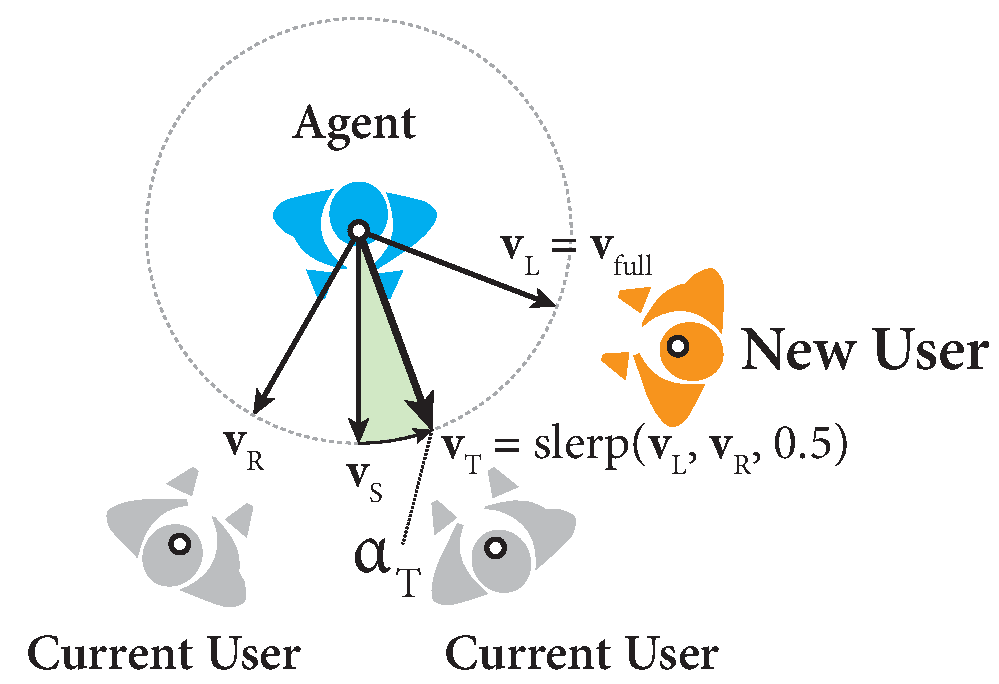
\includegraphics[width=0.75\textwidth]{conversationalrolegaze/Figures/FTorsoAlign.pdf}
\caption{Computing the torso alignment parameter $\alpha_T$ need for the agent to reconfigure the F-formation when a new user has joined the interaction.}
\label{fig:FTorsoAlign}
\end{figure}

To implement these behaviors, we use our gaze shift model (Chapter~\ref{cha:GazeShiftModel}) to execute the body orientation shifts. When the first user approaches the agent, the agent performs a gaze shift toward the user with the head, torso, and whole-body alignment parameters all set to 1 ($\alpha_H = \alpha_T = \alpha_B = 1$). This results in the agent facing the user head-on. If users are already present in the interaction, the agent must perform a gaze shift toward the new user that evenly distributes its body orientation among all the users. We set $\alpha_H = 1$ and $\alpha_B = 1$ as before, whereas $\alpha_T$ must be set such that the agent ends up oriented toward the midpoint between the leftmost and rightmost user. The procedure for computing $\alpha_T$ is as follows (Figure~\ref{fig:FTorsoAlign}). Let us define the following direction vectors:

\begin{enumerate}
\item $\mathbf{v}_S$ -- Current torso facing direction of the agent.
\item $\mathbf{v}_T$ -- Target torso facing direction of the agent.
\item $\mathbf{v}_\mathrm{full}$ -- Torso facing direction which would fully align the agent with the new user.
\item $\mathbf{v}_L$ -- Direction vector from the agent to the leftmost user.
\item $\mathbf{v}_R$ -- Direction vector from the agent to the rightmost user.
\end{enumerate}

All direction vectors are projected onto the horizontal plane. The agent must realign its body such that its torso facing direction ends up the following: $\mathbf{v}_T = \mathop{slerp}(\mathbf{v}_L, \mathbf{v}_R, 0.5)$. The torso alignment $\alpha_T$ needed to achieve that facing direction is:
%
\begin{align} \label{eq:FTorsoAlign}
\alpha_T = \frac{\angle(\mathbf{v}_S, \mathbf{v}_T)}{\angle(\mathbf{v}_S, \mathbf{v}_\mathrm{full})}
\end{align}
%

\subsection{Gaze Signalling of Footing}

We implement gaze behaviors for signaling footing based on~\citet{mutlu2012conversational}, who report probability distributions of participants' gaze among each other and the environment in scenarios with one addressee, two addressees, and one addressee with one bystander. According to their data, when there is a single addressee, the participants tend to spend only 26\% of the time looking at the addressee's face (making eye contact), while the rest of the time they avert their gaze toward the addressee's torso and the environment. The gaze aversions serve the purpose of intimacy regulation---eye contact is an arousal stimulus and staring into another person's eyes for long periods of time is known to cause discomfort~\citep{argyle1976gaze}. When a second addressee is present, the amount of gaze toward each addressee's face remains in the neighborhood of 26\%, but there is much less torso-directed gaze. This is likely because switching gaze among the addressees now also serves the purpose of intimacy regulation, so there is less need to gaze at the torso. Finally, if a bystander is present, participants only gaze at them 5\% of the time, or one fifth of addressee gaze amount.

In our implementation of footing-signalling gaze behaviors for virtual agents, we extrapolate the findings by~\citet{mutlu2012conversational} to support larger groups of addressees and bystanders. We define a discrete probability distribution over the set of gaze targets, which includes the faces and torso of all the addressees and bystanders, as well as the environment. The distribution is characterized by a probability mass function $p_T = p(T, N_A, N_B)$ (Table~\ref{tab:GazeFootingSpatial}), which specifies the probability of looking at the candidate target $T$ (addressee face or torso, bystander face or torso, or the environment) given the current configuration of user footing, consisting of $N_A$ addressees and $N_B$ bystanders. As the agent speaks or waits for a user to take the floor, it continually shifts its gaze between targets, which are chosen by drawing from $p_T$ (Table~\ref{tab:GazeFootingSpatial}). The temporal duration of each gaze fixation is then determined by drawing from a set of gamma distributions given in Table~\ref{tab:GazeFootingFixationLengths}.

\begin{table}
\centering
\def\arraystretch{1.5}
\begin{tabular}{|l|l|r|}
\hline
\textbf{Gaze Target} & \textbf{Footing Configuration} & \textbf{Gaze Probability} \\
\hline
\multirow{2}{*}{Addressee \emph{face}} & $N_A = 1$ & 26\% \\
& $N_A \geq 2$ & $54\%/N_A$ \\
\hdashline
\multirow{2}{*}{Addressee \emph{torso}} & $N_A = 1$ & 48\% \\
& $N_A \geq 2$ & $16\%/N_A$ \\
\hdashline
\multirow{2}{*}{Bystander \emph{face}} & $N_B = 1$ & 5\% \\
& $N_B \geq 2$ & $8\%/N_B$ \\
\hdashline
\multirow{2}{*}{Bystander \emph{torso}} & $N_B = 1$ & 3\% \\
& $N_B \geq 2$ & $5\%/N_B$ \\
\hdashline
\multirow{6}{*}{Environment} & $N_A = 1$, $N_B = 0$ & 26\% \\
& $N_A = 1$, $N_B = 1$ & 18\% \\
& $N_A = 1$, $N_B \geq 2$ & 13\% \\
& $N_A \geq 2$, $N_B = 0$ & 30\% \\
& $N_A \geq 2$, $N_B = 1$ & 24\% \\
& $N_A \geq 2$, $N_B \geq 2$ & 17\% \\
\hline
\end{tabular}
\caption{Spatial probability distribution of the agent's gaze while speaking or waiting for user speech, expressed as probability of looking at a target in the given configuration of conversational roles. $N_A$ is the number of addressees, while $N_B$ is the number of bystanders.}
\label{tab:GazeFootingSpatial}
\end{table}

\begin{table}
\centering
\def\arraystretch{1.5}
\begin{tabular}{|l|l|r|}
\hline
\textbf{Gaze Target} & \textbf{Footing Configuration} & \textbf{Fixation Length} \\
\hline
\multirow{3}{*}{Addressee \emph{face}} & $N_A = 1$, $N_B = 0$ & $\mathop{Gamma}(1.65, 0.56)$ \\
& $N_A = 1$, $N_B = 1$ & $\mathop{Gamma}(0.74, 1.55)$ \\
& $N_A \geq 2$ & $\mathop{Gamma}(1.48, 1.10)$ \\
\hdashline
\multirow{3}{*}{Addressee \emph{torso}} & $N_A = 1$, $N_B = 0$ & $\mathop{Gamma}(1.92, 0.84)$ \\
& $N_A = 1$, $N_B = 1$ & $\mathop{Gamma}(1.72, 1.20)$ \\
& $N_A \geq 2$ & $\mathop{Gamma}(1.92, 0.52)$ \\
\hdashline
Bystander \emph{face} & $N_B \geq 1$ & $\mathop{Gamma}(2.19, 0.44)$ \\
\hdashline
Bystander \emph{torso} & $N_B \geq 1$ & $\mathop{Gamma}(1.76, 0.57)$ \\
\hdashline
\multirow{3}{*}{Environment} & $N_A = 1$, $N_B = 0$ & $\mathop{Gamma}(0.90, 1.14)$ \\
& $N_A = 1$, $N_B = 1$ & $\mathop{Gamma}(1.84, 0.59)$ \\
& $N_A \geq 2$ & $\mathop{Gamma}(2.23, 0.41)$ \\
\hline
\end{tabular}
\caption{Agent's gaze fixation lengths (in seconds), expressed as gamma distributions specifying the length of fixation of a target in the given configuration of conversational roles.}
\label{tab:GazeFootingFixationLengths}
\end{table}

Consider an example: the agent is speaking with two addressees ($N_A = 2$) called  Alice and Bob, with two bystanders present ($N_B = 2$). When the time comes to shift the agent's gaze, we draw from the spatial probability distribution to determine the target of the gaze shift. According to Table~\ref{tab:GazeFootingSpatial}, the probability of looking at Alice's face is $54\% / 2 = 27\%$ (second row); let us assume this is the target we have chosen by randomly drawing from the distribution. Next, we need to determine how long to fixate the gaze on Alice's face. We generate the fixation length by drawing from the distribution $\mathop{Gamma}(k = 1.48, \Phi = 1.10)$ (Table~\ref{tab:GazeFootingFixationLengths}, third row).

Since~\citet{mutlu2012conversational} only provide data for interactions with two addressees or one addressee and one bystander, we had to extrapolate gaze probabilities to 3+ addressees and 2+ bystanders. Our extrapolated distribution is based on the idea that the total probability of the agent looking at addressees is a constant 70\%. This probability is then equally divided among individual addressees, so if $N_A = 3$, the probability of looking at any one addressee is 23\%. The latter probability is the sum of probabilities of looking at the addressee's face (18\%) versus their torso (5\%). It implicitly follows from Table~\ref{tab:GazeFootingSpatial} that the ratio of face and torso probabilities is also constant. By the same token, we extrapolate the probabilities of looking at bystanders. If we have 2+ bystanders, the total probability of looking at them is a constant 13\%, which gets equally divided among them.

One question we have not touched upon is: what happens when the gaze target is in the environment? The probability distribution in Table~\ref{tab:GazeFootingSpatial} tells us the probability of looking at \emph{any} location in the environment, but it does not tell us \emph{what} that location is. We use a procedure inspired by~\citep{mutlu2012conversational} to determine the target location $\mathbf{p}_E$ in the environment. First, we predefine a set of $n$ target locations around each user---typically located to their left, right, and front (at their feet). We label these locations $\mathbf{p}_{E,i}$, where $i = [1..n]$. If by drawing from the spatial probability distribution we have determined that the agent's next gaze target is in the environment, we choose among the $n$ candidate locations around the \emph{currently gazed-at user} with uniform probability. Let us assume we have chosen the $k$-th location. We determine the exact 3D position $\mathbf{p}_E$ by drawing from a clipped, spherical normal distribution centered on $\mathbf{p}_{E,k}$: $\mathbf{p}_E = \mathbf{p}_{E,k} + N(0, \sigma = R/2)$. $R$ is the radius of the sphere around $\mathbf{p}_{E,i}$ to which the normal distribution is clipped---we set this to 37 cm in our implementation.

\subsection{Other Gaze Cues}

The agent uses the gaze behaviors for footing while it is speaking or while waiting for a user to speak (i.e., after releasing the floor.) It also uses several other patterns that complement or override those. Firstly, when beginning a speech utterance, the agent always looks into the face of the addressee; if there are multiple addressees, the agent randomly chooses between them. Secondly, at the end of the utterance, the agent always looks back at the addressee's face as it releases the floor to them. Thirdly, while a user is speaking, the agent is always looking at their face, with frequent gaze aversions generated using the Eyes Alive model~\citep{lee2002eyes}. 

\section{Evaluation}
\label{sec:GazeFootingExperiment}
Having designed and implemented our gaze behaviors, we conducted a study with human participants, which aimed to answer the following research question: ``Can a virtual agent use its nonverbal cues---gaze and body orientation---to shape the footing of participants in multiparty interactions in a virtual environment?'' In our study, we had human participants engage in short, 10-minute conversations with a virtual agent and a simulated, avatar-embodied confederate. The participants would either experience the conversation on a 2D display or they would be immersed in the virtual environment using a VR headset. The virtual agent displayed gaze patterns and body orientation shifts that would either include the participant as an addressee or exclude them as a bystander. Our primary goal was to show that the participant would conform to the conversational role signaled by the agent's footing cues---e.g., when assigned the role of bystander, the participant would converse less with the agent. Our secondary goal was to show that these effects would be augmented in a virtual reality setting, where participants would have a better spatial awareness of their conversational partners' nonverbal cues.

\subsection{Hypotheses}

We designed a study to test the following hypotheses:

\begin{enumerate}
\item Participants will demonstrate conversational behavior that conforms to their footing as signaled by the agent's gaze and body orientation cues. Participants assigned the role of addressees will take more and longer speaking turns. This is consistent with research on human conversational behavior, which shows that conversing partners tend to orient themselves in an particular arrangement called F-formation~\citep{kendon1990conducting} and that people tend to look at the addressees of their utterances~\citep{kendon1967some}.
\item Participants will evaluate the agent more positively if they are assigned the role of addressees rather than bystanders. This is consistent with findings that people who make a lot of eye contact are viewed as more likeable and credible~\citep{argyle1976gaze,beebe1976effects}.
\item Participants will feel more groupness if they are assigned the role of addressees, because reduced gaze toward bystanders will lead to feelings of ostracism and exclusion~\citep{wirth2010eye}.
\item The agent's footing cues will have a stronger effect on the participants' conversational behavior (Hypothesis 1) in the VR setting than when using a 2D display.
\item The agent's footing cues will have a stronger effect on the participants' subjective perceptions of the agent (Hypothesis 2) in the VR setting than when using a 2D display.
\item The agent's footing cues will have a stronger effect on the participants' feelings of groupness (Hypothesis 3) in the VR setting than when using a 2D display.
\end{enumerate}

\subsection{Design}

The study followed a 2x2 mixed factorial design. The independent variables were \emph{agent behavior} and \emph{task setting}. The agent behavior variable was between-participants and had the following levels:

\begin{enumerate}
\item \emph{Exclusive} -- The agent displayed nonverbal behaviors that would exclude the participant from the interaction as a bystander. It would orient its body toward the confederate (facing them straight-on) and gaze at them much more than at the participant, in accordance with the distributions given in Table~\ref{tab:GazeFootingSpatial}.
\item \emph{Inclusive} -- The agent displayed nonverbal behaviors that would include the participant in the interaction as an addressee. It would distribute its body orientation evenly between the participant and the confederate (using the mechanism depicted in Figure~\ref{fig:FTorsoAlign}, and gaze at them equally (Table~\ref{tab:GazeFootingSpatial}).
\end{enumerate}

Figure~\ref{fig:GazeFootingConditions} illustrates the agent behavior manipulation. Images on the left show the conversational formations resulting from agent's body orientation shifts at each level of the manipulation, whereas the right images show the views of the scene from the participant's perspective.

The other independent variable, task setting, had the following levels:

\begin{enumerate}
\item \emph{2D Display} -- The participant experienced the interaction on a 27\" Dell monitor, at 2560x1440 resolution and 50$^\circ$ field of view, while using the mouse to control their viewpoint.
\item \emph{VR} -- The participant wore a VR headset (Oculus Rift CV1). They saw the scene at the resolution of 1080x1200 per eye, with a 110$^\circ$ field of view. Built-in head orientation tracking and the external positional tracker allowed the participant to control their viewpoint by moving their head.
\end{enumerate}

The screenshots in Figure~\ref{fig:GazeFootingConditions} are both from the \emph{2D Display} condition. The use of the Oculus Rift in the \emph{VR} condition afforded a much higher field of view and more natural control over the viewpoint, allowing the participant to easily see both the agent and the confederate simultaneously, as well as shift their gaze from one to the other by simply moving their head.

Since the study had a within-participants factor, we implemented two versions of the task to minimize transfer effects. The tasks were identical in structure and duration, and they had similar content. The participants were assigned to conditions in stratified order, counterbalanced with respect to task setting (\emph{2D Display} or \emph{VR}) and task version (\emph{Task 1} or \emph{Task 2}).

\subsection{Task}

The study task was a three-party interaction in a virtual room. The interaction took the form of a casual, interview-style conversation moderated by the agent. The conversational partners were the agent, the participant, and a simulated, avatar-embodied confederate. At the start of the task, the participant would find themselves standing at the room's entrance with a view of the agent and confederate on the other side of the room (Figure~\ref{fig:GazeFootingTask}, left); the agent and confederate would face each other in a vis-a-vis formation. The participant was prompted to click a button (either on the mouse or the Oculus Remote) to initiate the interaction; upon doing so, the camera would automatically approach the agent. Depending on the agent behavior condition, the agent would either glance at the participant and continue facing the confederate (\emph{exclusive} agent behavior) or reorient itself toward the participant (\emph{inclusive} agent behavior, Figure~\ref{fig:GazeFootingTask}, middle).

After introducing herself and greeting the partners, the agent would begin asking casual questions about their life experiences and interests. Some questions were designed to elicit short, one-sentence responses (e.g., ``What is your favorite movie?''), while others elicited longer, more open-ended responses (e.g., ``What is your favorite movie about?'') Most questions were implicitly addressed at both the participant and confederate, and they both had a choice in answering them. Our expectation was that the participant was more likely to take the conversational floor and answer the question if the agent demonstrated more inclusive nonverbal behaviors. A speech recognition system was used to detect when the participant was speaking; while the participant was speaking, the agent would look at them.

The confederate was simulated and its behavior entirely scripted. At the end of the agent's turn, the system would randomly decide if the confederate should answer the current question or not. If yes, the confederate would take the floor within about 0.75 $s$ and give a prerecorded response to the question. If not, the system would wait up to 3.4 $s$ for someone to speak out; if no one did, either the confederate would take the floor and answer, or the agent would proceed with the next question. The pause values between turns are derived from measurements of human speech in prior work and padded for possible speech recognition lag. According to~\citet{weilhammer2003durational}, the mean pause between turns is about 380 $ms$ in spontaneous American-English discourse, whereas silences longer than 3 $s$ are experienced as uncomfortable~\citep{mclaughlin1982awkward}.

\noindent\emph{Setup} -- The physical setup of the task is shown in Figure~\ref{fig:GazeFootingTask}, right. Participants were seated in an office chair in front of a personal computer while wearing an audio headset (in the \emph{2D Display} condition) or Oculus Rift (in the \emph{VR} condition). A video camera was set up to record their behavior.

\noindent\emph{Implementation} -- The task was implemented in Unity game engine. The task logic, agent's conversational behaviors, and task measurements were all implemented in C\# scripts. Microsoft Speech SDK was used for speech detection and the agent's speech synthesis and lip-sync, while Oculus Lip Sync was used to animate the confederate's lip movements. The agent and confederate character models were imported from DAZ~\citep{daz3d}. Both models had a looping, idle body animation applied to enhance the naturalness of their behavior.

\subsection{Participants}

We recruited 32 participants (17 female and 15 male) through an online student job website as well as in-person recruitment. All participants were students. 27 participants were native English speakers.

\subsection{Procedure}

We conducted the experiment in a small, closed study room with a computer table. The participants were ushered into the room by the experimenter and seated at the table. Following a brief overview of the task, they were given a consent form to read and sign. Next, they were given detailed task instructions and handed an instructions sheet to serve as a reminder. The experimenter would then launch the task application and leave the room. Upon task completion, the participants were handed a questionnaire for subjective evaluation of the agent and task. This was followed by a second trail of the task, upon which the participants would fill out another subjective questionnaire and a brief demographics questionnaire. Finally, the participant received payment in the amount of \$5. Total experiment duration was 30 minutes.

\subsection{Measures}

Our experiment involved two behavioral and four subjective measures. The behavioral measures were the following:

\begin{enumerate}
\item \emph{Number of speaking turns} -- Total number of speaking turns taken by the participant over the course of the interaction.
\item \emph{Speaking turn length} -- Mean length of speaking turns taken by the participant.
\end{enumerate} 

The behavioral measures served as measures of participation. We expected that the participant would take more and longer speaking turns if the agent looked at them more.

The subjective measures were collected using the subjective questionnaire. 



\section{Discussion}
\label{sec:GazeFootingDiscussion}
The current chapter has presented the design of effective gaze and body reorientation behaviors enabling a virtual agent to reconfigure the conversational formation and signal footing to human users in order to shape their speaking behavior---eliciting conversational contributions from them as addressees or excluding them as bystanders. The presented study with human participants has demonstrated that a virtual agent equipped with these behaviors has the capability to influence users into conforming with their conversational role, which manifests itself specifically in the immersive VR setting. The effectiveness of the proposed behaviors in immersive VR is likely due to participants' increased awareness of the spatial arrangement of the interaction and the agent's gaze cues.

This work motivates the importance of coordinated gaze and body orientation in signaling attention and supporting high-level processes in multiparty interaction with a virtual agent. It also underscores that such capabilities are only going to become more important as consumer VR takes hold and multiparty interactions become an integral part of social VR experiences. However, it only represents a first step in terms of improving agents' nonverbal behaviors to the point of enabling them to autonomously and effectively manage interactions with multiple users within a virtual space. For one, body reorientation is insufficient to effect reconfigurations of the conversational formation as users join and leave the interaction---the agent also needs the ability to move to a different position and account for obstacles in the environment. This would also afford control over the effects of proxemics: as the results of our experiment suggest, inappropriate personal distance can have a negative impact on user experience. Finally, the agent needs to react to user behaviors and infer their engagement intent from their movements---i.e., before engaging with the user as an addressee, it should first understand if that user even desires such a level of engagement or if they prefer to remain on the sidelines as a bystander. Such problems have been explored in the context of physically situated interaction with embodied agents~\citep{bohus2009models}, but they are beyond the scope of the current work.

\chapterstyle{deposit}
\pagestyle{deposit}

\chapter{Stylized and Performative Gaze}
\label{cha:StylizedGaze}

\section{Introduction}
\label{sec:StylizedGazeIntro}
The preceding chapters have introduced methods for controllable synthesis of directed gaze shifts and demonstrated their use as building blocks of effective conversational behaviors for interactive virtual agents. The ability to synthesize humanlike behaviors in a controllable fashion is a necessary, but insufficient prerequisite for creating character animation.
To synthesize or author believable motion in a scalable way, one also requires the ability to apply that motion to characters with different designs. The objective of character animation is to tell stories and those stories can involve characters of varying shapes, sizes, and species. In particular, stylized and anthropomorphic characters are found across many media, such as film and television animation, video games, and instructional content for children. As discussed in Section~\ref{sec:AnimatingStylizedCharacters}, automatically producing high-quality animation for such characters is a challenging and underexplored problem.

\begin{figure}
\centering
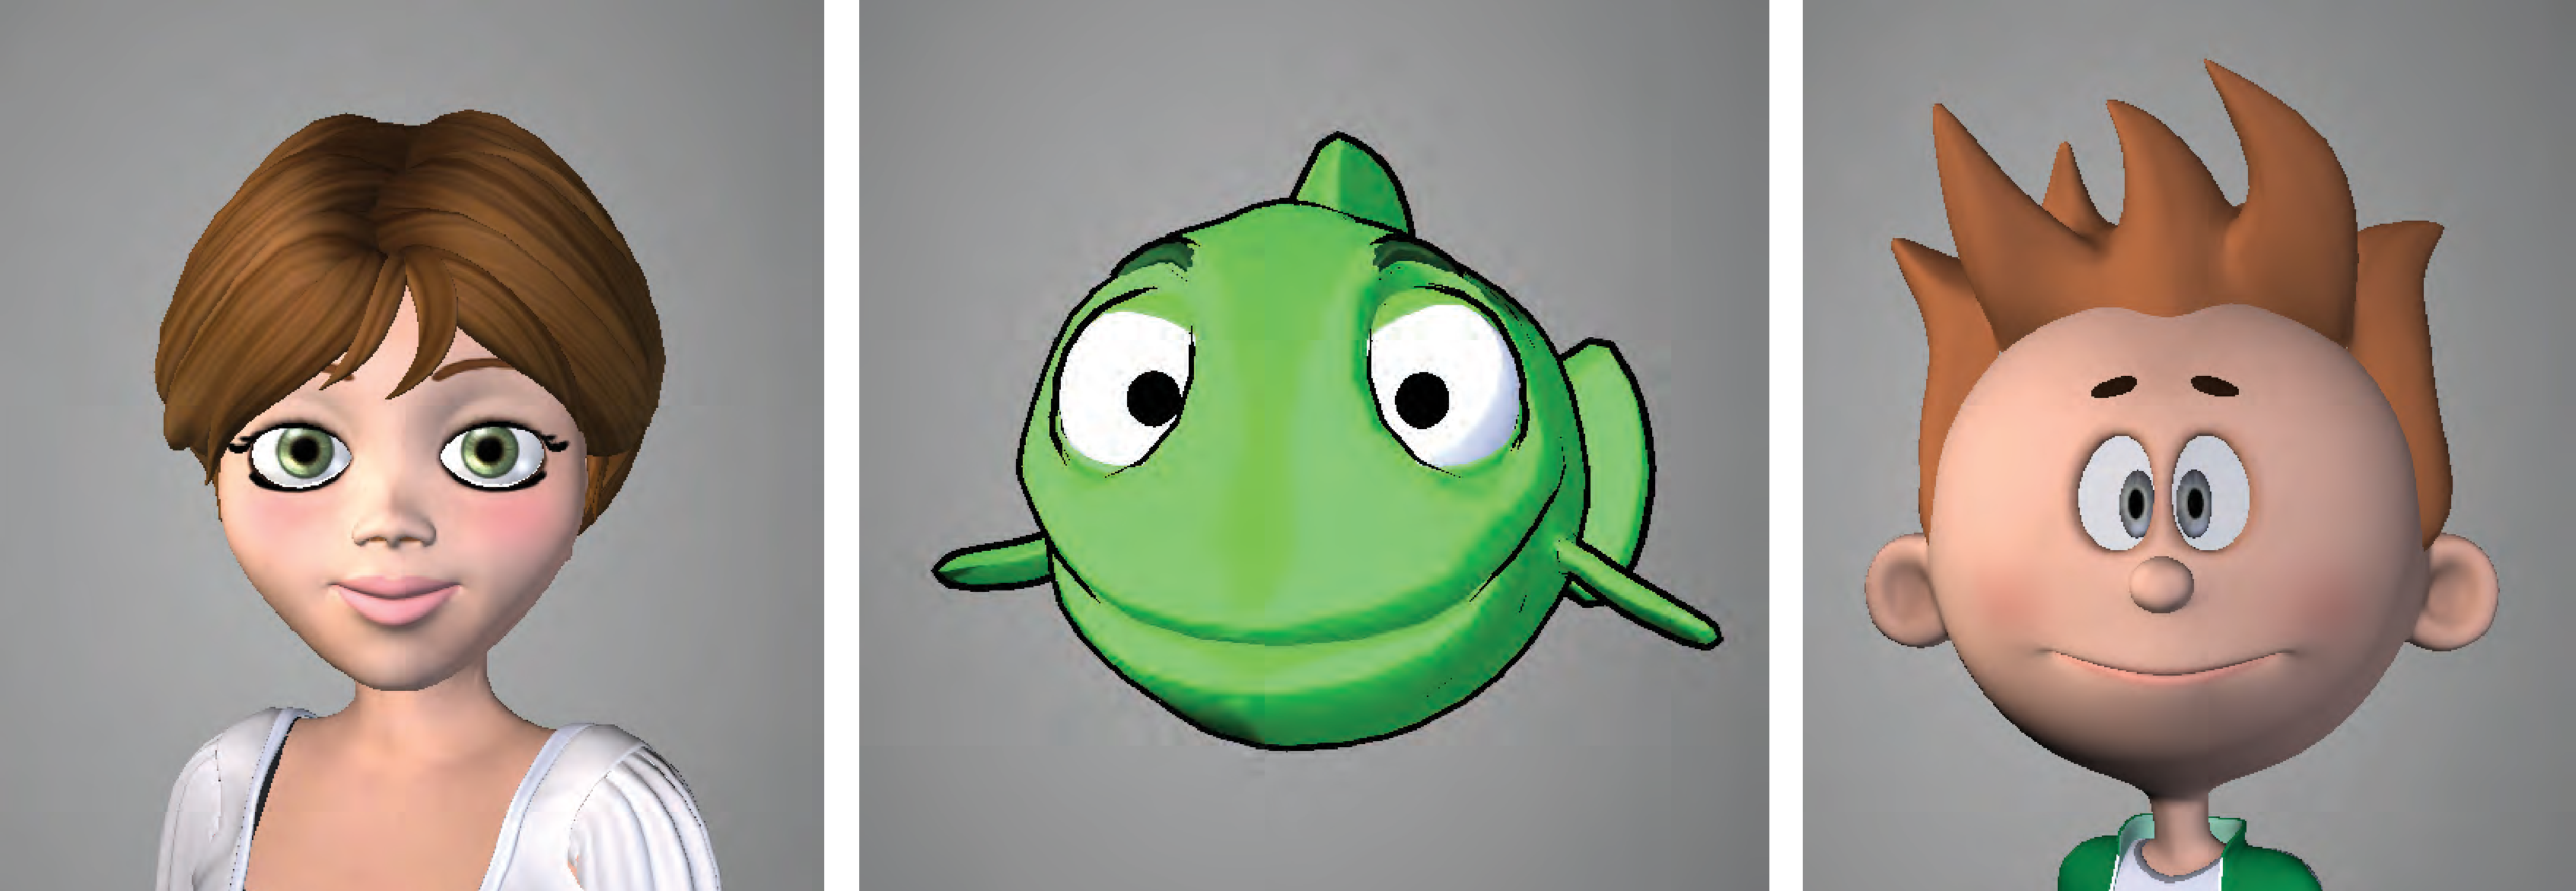
\includegraphics[width=0.85\textwidth]{stylizedgaze/Figures/StylizedCharacterExamples-small.pdf}
\caption{Examples of stylized characters. Characters 1 and 2 have large eyes and high inter-eye distance. Characters 2 and 3 have asymmetric eye motor range (OMR). Character 3 has narrow OMR and low inter-eye distance.}
\label{fig:StylizedCharacterExamples}
\end{figure}

The extent of this challenge is evident in the domain of gaze animation as well. Established methods for directed gaze animation have limited applicability to stylized characters; these methods are designed to simulate human gaze movements, so they implicitly incorporate human anatomic and neurophysiological constraints. Stylized characters tend to have exaggerated geometry with large and often asymmetrically shaped eyes such as those depicted in Figure~\ref{fig:StylizedCharacterExamples}. Applying models of realistic human gaze motion to such characters can result in aesthetically and communicatively poor animation. Enlarged and often asymmetric eye anatomy can magnify subtle phenomena of human gaze that are normally unnoticeable (e.g., cross-eyedness resulting from vergence) and lead to biologically implausible movements (e.g., one eye moving while the other is stationary.) Such gaze animation artifacts can appear unpleasant, distracting, and alter the communicative intent of the gaze behavior. In this chapter, I propose a set of online motion adaptation methods for reducing artifacts in gaze motion on stylized characters; I call these methods \emph{stylized gaze}. They are implemented as extensions of the gaze shift model described in Chapter~\ref{cha:GazeShiftModel}.

A secondary constraint of established gaze shift models is of a utilitarian variety: these models require the eyes to align exactly with the gaze target. The basis for this requirement seems obvious. For people, gaze has perceptual utility---it enables us to see objects and other people. If human gaze always lines up with its target in the environment, why not require the same of virtual characters' gaze?
However, when we look beyond everyday usage of gaze, we realize there are many situations when people do not look in order to see.
In visual storytelling media, such as theater, film, and cartoon animation, the primary purpose of gaze is to communicate ideas to the audience. The actor's line of sight does not always align with the target they are ``looking'' at. Actors often look only in the general direction of the target, while maintaining the orientation of their body toward the camera or audience. The audience can more clearly see what the actor is attending to, even if their line of sight is not actually aligned with the target.
I dub this partially aligned, viewer-oriented gaze behavior \emph{performative gaze}. The technique has a basis in human perception---people are notoriously imprecise at estimating the gaze direction of others, unless they themselves are being looked at~\citep{argyle1976gaze}. In this chapter, I propose a method for automatic adaptation of gaze shift motion relative to the viewpoint (i.e., camera position), allowing an animator to achieve performative gaze through the manipulation of a single parameter.

The remainder of the chapter is organized as follows: I give an overview of animation artifacts that occur when applying humanlike gaze shift movements to stylized characters (Section~\ref{sec:StylizedGazeArtifacts}), I present the stylized gaze methods for the adaptation of gaze shift movements to stylized characters (Section~\ref{sec:StylizedGazeAdaptation}), and I present the performative gaze method for adaptation of gaze shift movements relative to the viewpoint (Section~\ref{sec:PerformativeGaze}). Finally, I demonstrate how the proposed methods lead to reduction of undesirable artifacts in gaze motion without compromising the communicative effectiveness of gaze shifts (Sections~\ref{sec:StylizedGazeEvaluation1} and~\ref{sec:StylizedGazeEvaluation2})\footnote{This chapter was published in~\citet{pejsa2013stylized}.}. 

\section{Artifacts on Stylized Characters}
\label{sec:StylizedGazeArtifacts}
State-of-the-art models for gaze shifts incorporate features of human anatomy, including eye dimensions, inter-eye distance, and symmetry of oculomotor range. When such models are applied to a stylized character with exaggerated or non-human anatomic features, we observe two kinds of phenomena. First, anatomically correct, but rarely observed, elements of human gaze can be magnified and become noticeable. Second, asymmetry and exaggerated size of the eyes can cause anomalous situations that are rare or impossible in healthy human gaze. We argue that these phenomena are undesirable, as they can distract the viewer and/or alter the semantics of the gaze shift. Below, we catalog specific visual artifacts that our gaze model seeks to address. 
%Many of these artifacts are difficult to convey in static images, please refer to the video supplement for better illustrations.

\begin{figure}[!b]
\centering
\vspace{-6pt}
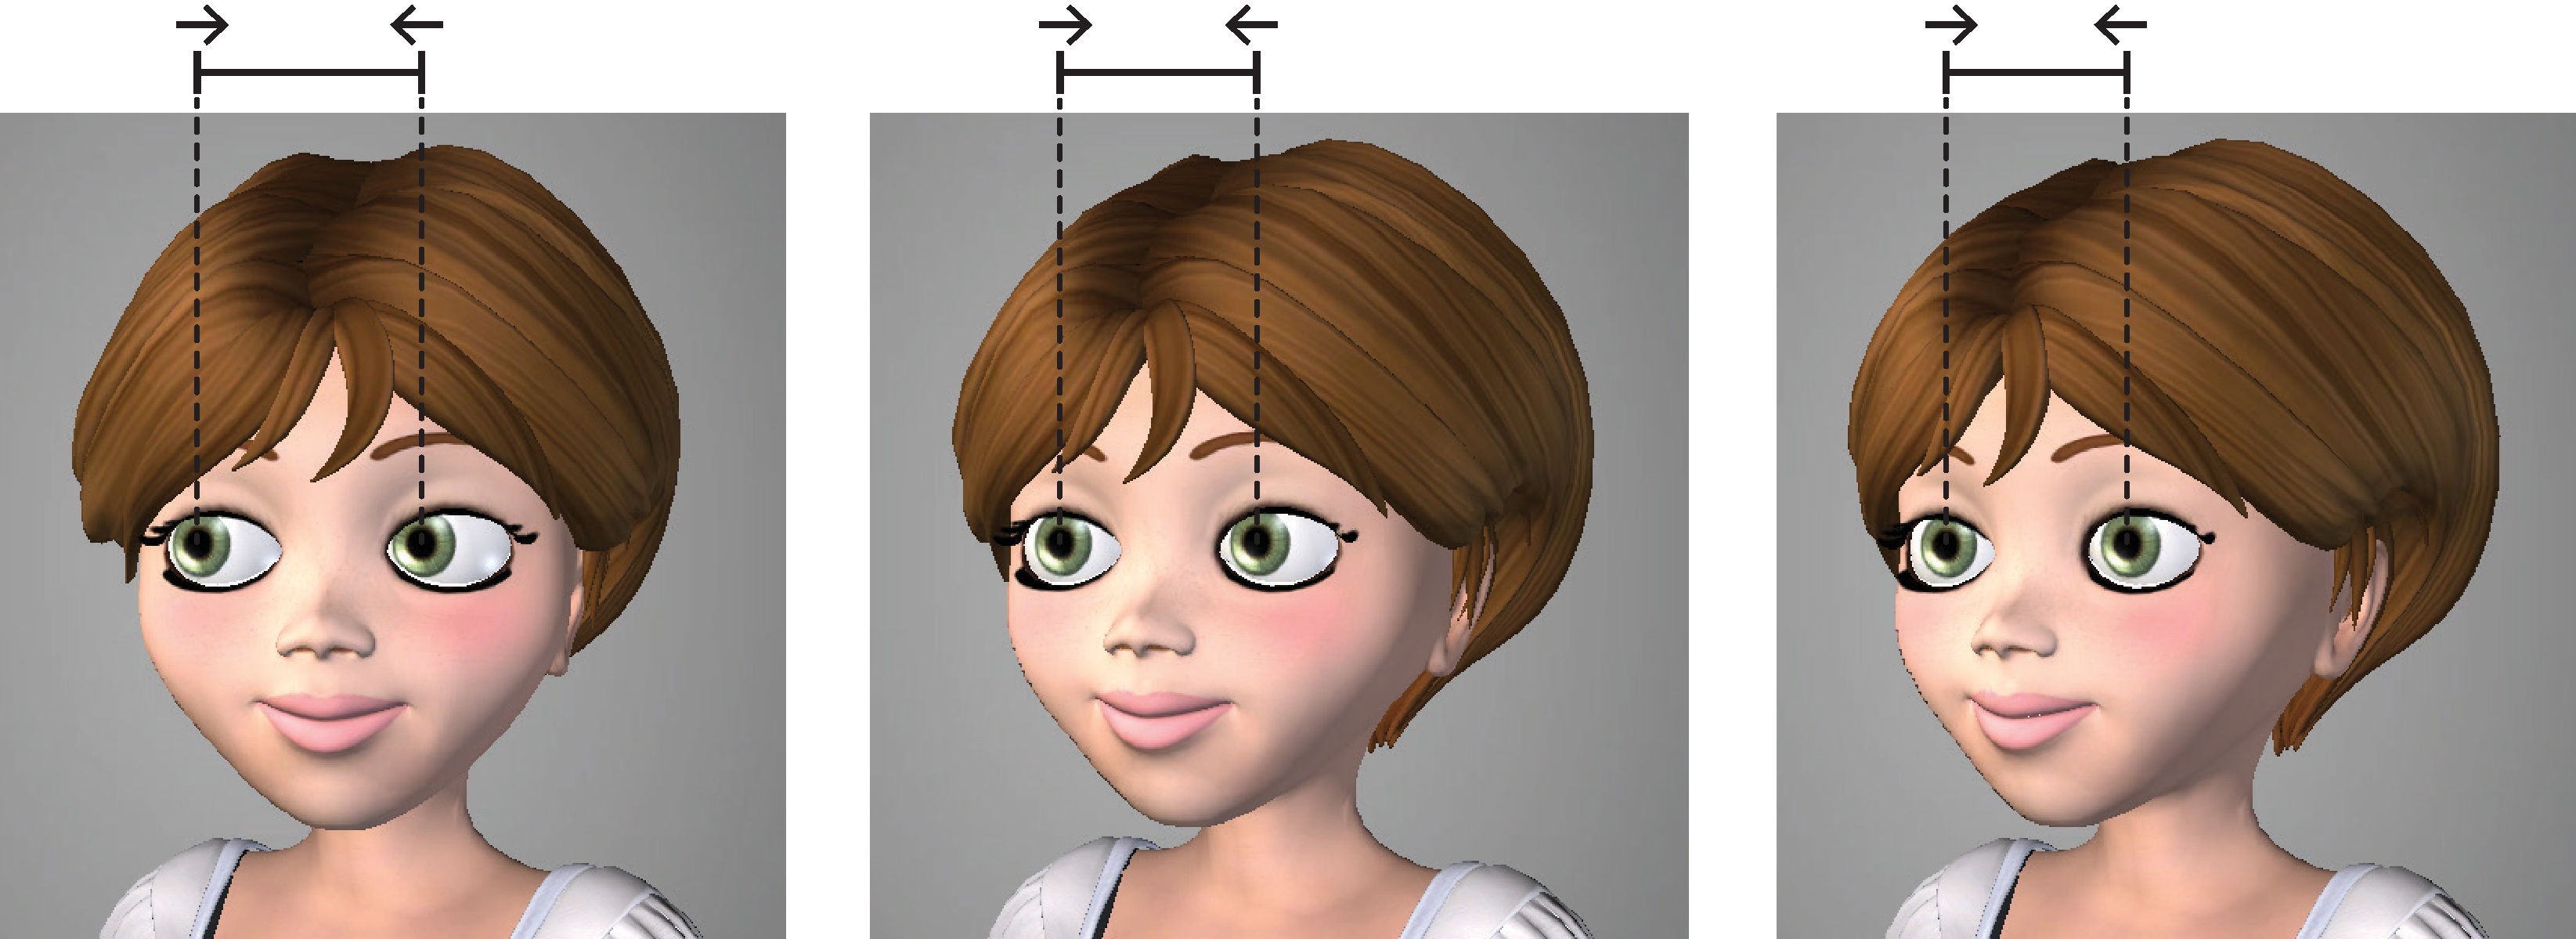
\includegraphics[width=0.48\textwidth]{Figures/EyeRetractionExample-small.pdf}
\caption{Eye retraction example. The right eye has aligned with the target and is retracting as the left eye moves forward. Notation: Solid line indicates inter-eye distance. Arrows $\rightarrow$ and $\leftarrow$ indicate eye movement direction.}
\vspace{-6pt}
\label{fig:EyeRetractionExample}
\end{figure}
% NOTE: Added better notation to all figures, and explanation in the caption of this one -- Tomislav

\begin{figure}[t]
\centering
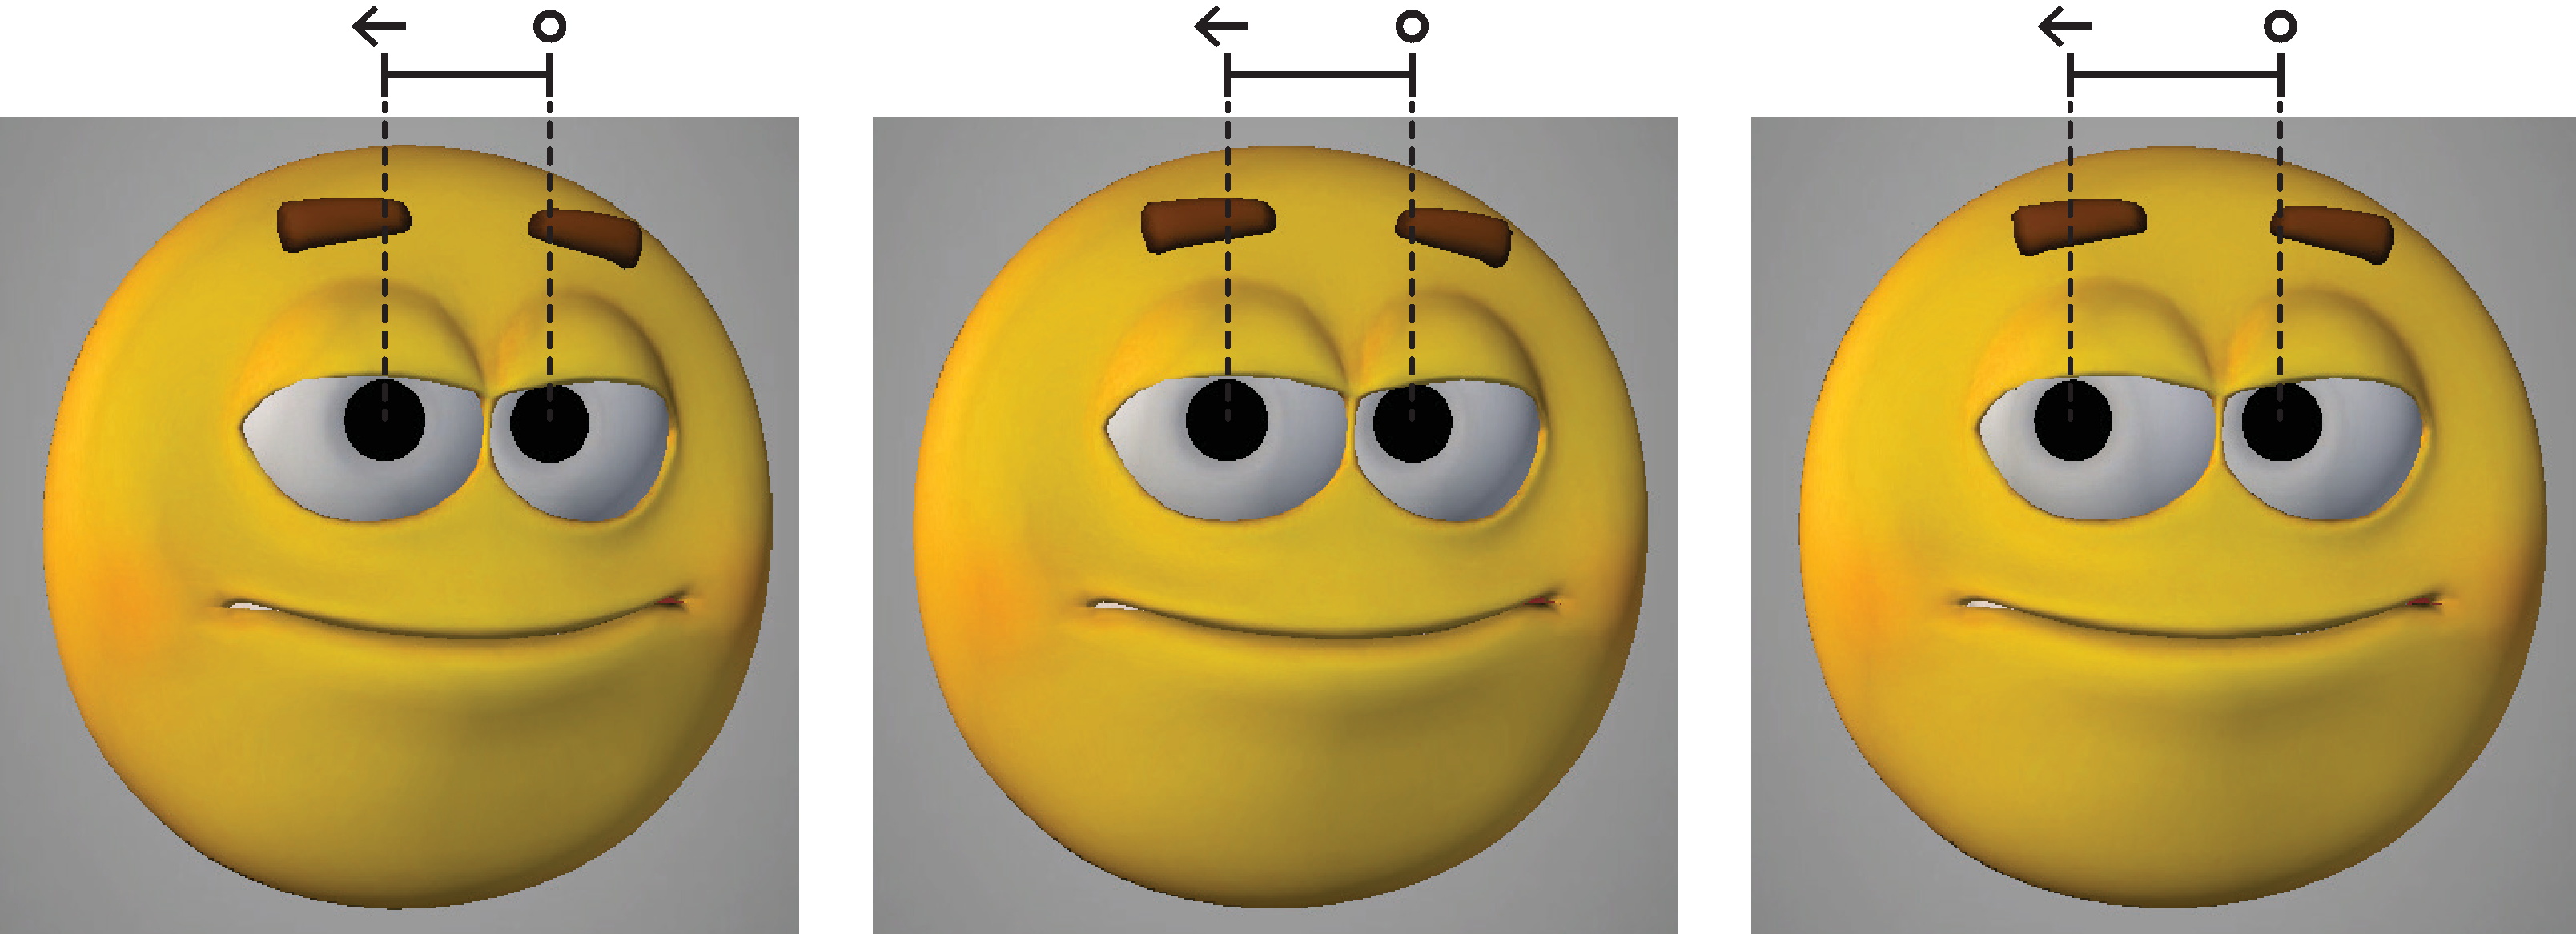
\includegraphics[width=0.48\textwidth]{Figures/StuckEyeExample-small.pdf}
\caption{Stuck eye example. The right eye is moving ahead, while the left eye is blocked by OMR. Notation: Dot $\circ$ indicates that the eye is stationary.}
\vspace{-10pt}
\label{fig:StuckEyeExample}
\end{figure}

\noindent\emph{Cross-eyedness} -- Cross-eyedness occurs when the eyes significantly angle inward (towards each other). In humans, while convergence on a target necessitate some amount of inward angle, excessive amounts are straining to maintain. Small amounts of cross-eyedness are not noticeable due to the small size of the eyes, and larger amounts are caused by unnatural viewing conditions or an explicit expression. In characters with large or widely spaced eyes, cross-eyedness becomes noticeable even in more standard viewing (Figure~\ref{fig:CrosseyednessFixExample}).

\noindent\emph{Speedy eyes} -- Human eyes have low mass and strong muscles that support fast and abrupt movements. In characters with larger eyes, such movements can appear implausible.

\noindent\emph{OMR-block} %(Figure~\ref{fig:OMRBlockExample})
--  When the eyes initiate a gaze shift and reach the boundary of the \textit{ocular motor range} (OMR), they are effectively blocked in their movements until the head brings them into alignment with the gaze target. While natural and common in humans, this phenomenon can appear anomalous in stylized characters; during this prolonged phase when the eyes are unable to move, the character may appear static and puppet-like. We believe this phenomenon to be caused by \textit{speedy eyes}; the eyes cover the distance between starting position and OMR in an unrealistic speed, resulting in an unusually long period of OMR-block. The visual artifact becomes even more prevalent with narrow OMR, a common property of stylized characters.

\noindent\emph{Eye retraction} -- In human gaze, when the head brings the eyes into alignment with the gaze target, the \textit{vestibulo-ocular reflex} (VOR) effectively locks the eyes onto the target as the head catches up, rotating the eyes in the opposite direction of the head movement. While this standard feature of human gaze does not appear as anomalous in real humans or characters with humanlike proportions, in stylized characters with large eyes, it can appear as if the eyes have overshot the target and are now suddenly retracting in order to realign with it (Figure~\ref{fig:EyeRetractionExample}). We believe that the cause of this illusion is excessive eye velocities that cause the eyes to advance further ahead and retract more than expected.

\noindent\emph{Stuck eye} -- Stuck eye is caused by asymmetry of eye shape, which necessarily involves asymmetry in the OMR. The leading eye in the gaze shift, which rotates outward, has a greater distance to cover before reaching OMR than the trailing eye. However, when both eyes move at the same velocity, as is the case with human eyes, the trailing eye will reach its OMR boundary sooner and become blocked, while the other eye will continue moving (Figure~\ref{fig:StuckEyeExample}). Movement in one eye does not occur in human gaze except in medical conditions such as amblyopia and therefore can appear abnormal.

\noindent\emph{Eye divergence} -- When the eyes have asymmetric OMR, their gaze directions can become divergent as they reach their respective OMR boundaries. Although difficult to observe in static poses, this divergence might cause disconjugate eye movements and appear jarring when the eyes are brought into alignment with the gaze target. In these movements, the leading eye will reach the gaze target before the trailing eye, and VOR causes the eye to rotate backward, while the trailing eye is still moving forward (Figure~\ref{fig:EyeDivergenceFixExample}). %This draws attention to the fact that eye orientations were divergent in the first place. 
Such divergent orientations and movements are improbable in healthy human gaze and appear anomalous.

\section{Gaze Adaptation}
\label{sec:StylizedGazeAdaptation}
To enable believable animations of gaze shifts on stylized and non-human characters, we propose a set of motion adaptation methods and implement them as extensions of the gaze shift model described in Chapter~\ref{cha:GazeShiftModel}. The methods are designed to explicitly reduce the prevalence of artifacts described in the previous section, while seeking to maintain as much of the human movement as possible. The proposed methods fall into three categories.
First, we introduce changes to how the target pose of the eyes and head is computed in order to prevent the occurrence of anomalous poses. Second, we extend the computation of eye movement kinematics to account for variable physical constraints of the exaggerated geometries that are common in stylized characters. Third, we manipulate the timings of gaze-evoked eye blinks to co-occur with potential visual artifacts in order to conceal them.

To specify the character's anatomic and neurophysiological properties, we introduce four animator-adjustable parameters to the model. Eye width, $W$, is the width of the eye as a factor of the width of the typical human eye (approximately $2.5 cm$), ranging from 1 to 3 in the characters used in our examples. Eye strength $F$ allows for tuning the strength of the character's eye muscles relative to that of a human. Additionally, we replace the single parameter of the $OMR$ in humans with parameters $OMR_{IN}$ and $OMR_{OUT}$ that afford asymmetric eye motion by specifying the inward and outward OMR limits (in angle degrees), respectively. Eye width, $W$, and OMR parameters, $OMR_{IN}$ and $OMR_{OUT}$, can be determined from face geometry. We compute the eye strength automatically from the eye width as $F = W^3/3$; this works well across a range of characters.

\subsection{Target Pose Adaptation}
\label{sec:StylizedGazeTargetPoseAdaptation}

Models for humanlike gaze shifts, when applied to a stylized character with large eyes, are prone to bring the eyes into a noticeably cross-eyed state. If the character's eyes are asymmetric, then the eyes can also be led into a divergent state, which will become noticeable as the leading eye reaches the gaze target and the VOR reverses its direction of movement. To avoid these artifacts, we propose methods that adapt the target pose of the eyes and head at the beginning of the gaze shift by adjusting the effective gaze target position and the OMR parameters.

\subsubsection{Cross-eyedness Removal}

\begin{figure}
\centering
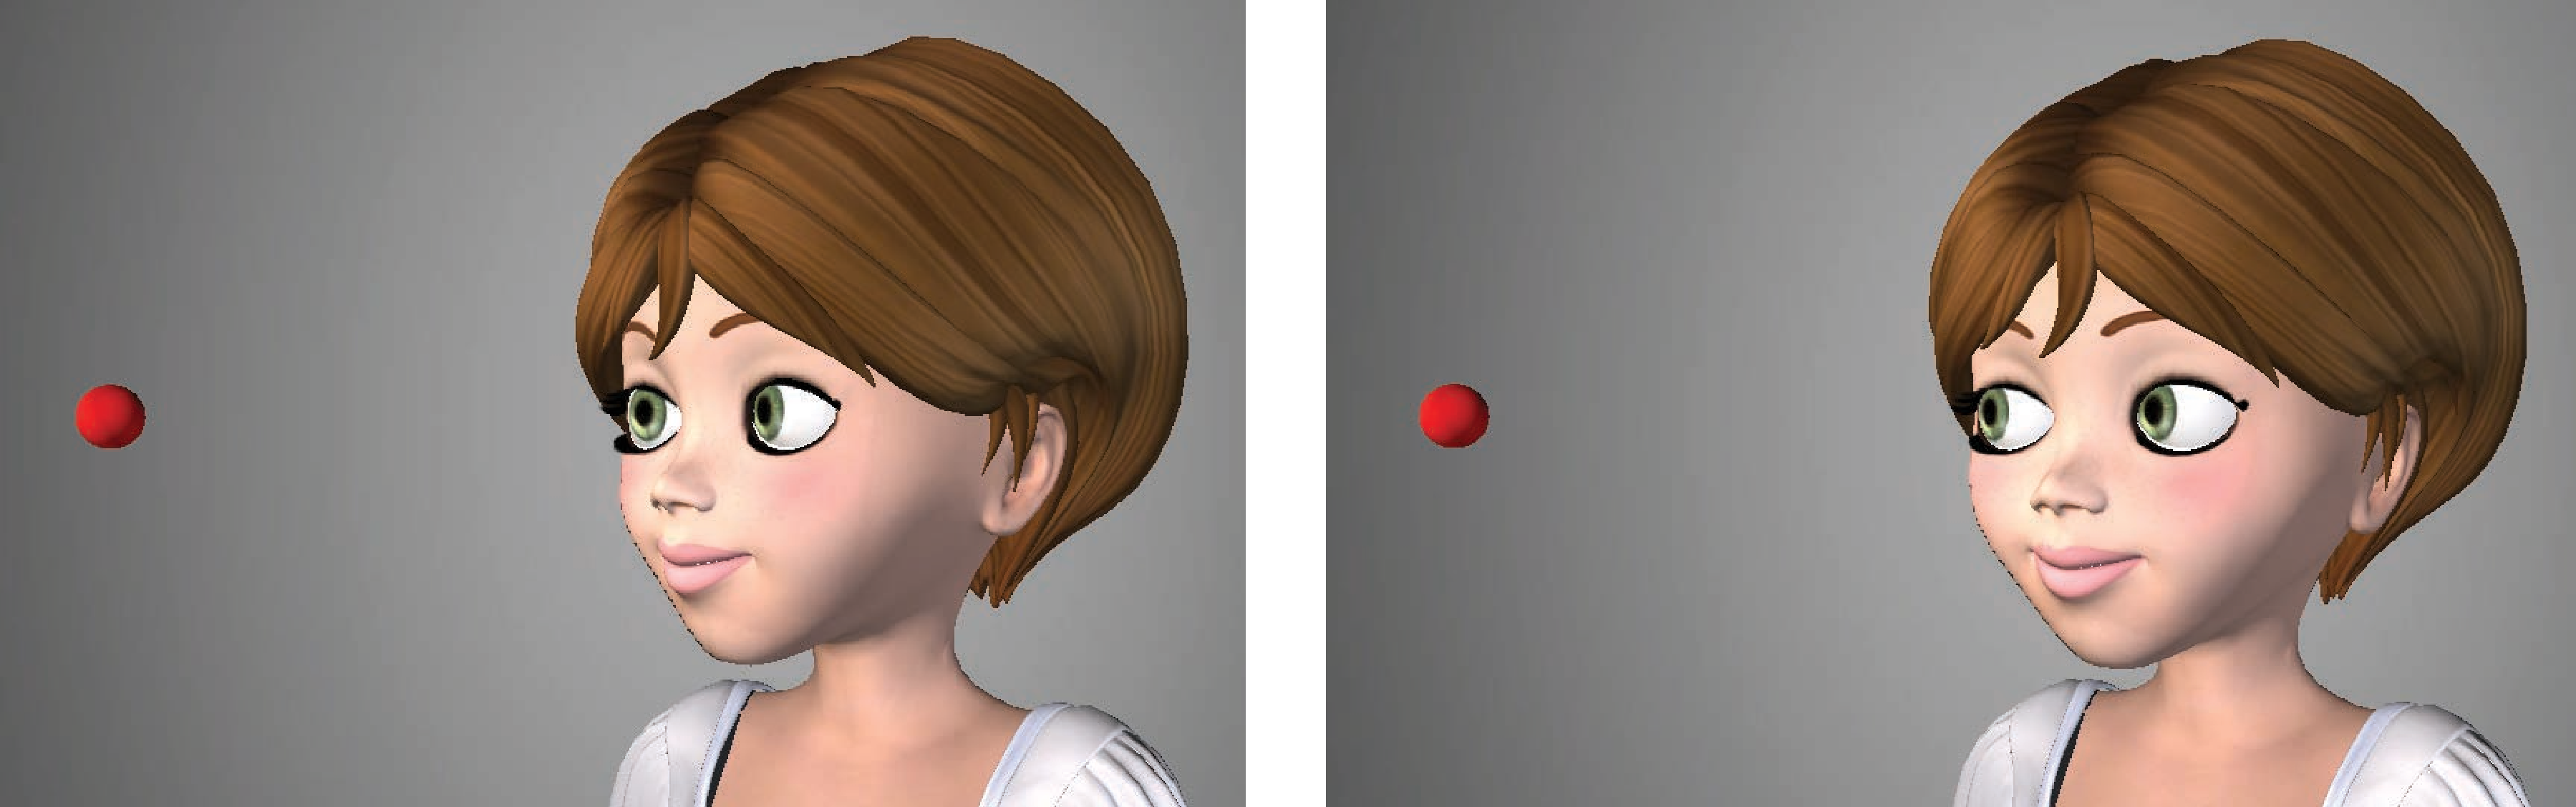
\includegraphics[width=0.85\textwidth]{stylizedgaze/Figures/CrosseyednessFixExample-small.pdf}
\caption{Cross-eyedness and its reduction. Left: Cross-eyed character. Right: Cross-eyedness reduced by our method.}
\label{fig:CrosseyednessFixExample}
\end{figure}

\begin{figure}
\centering
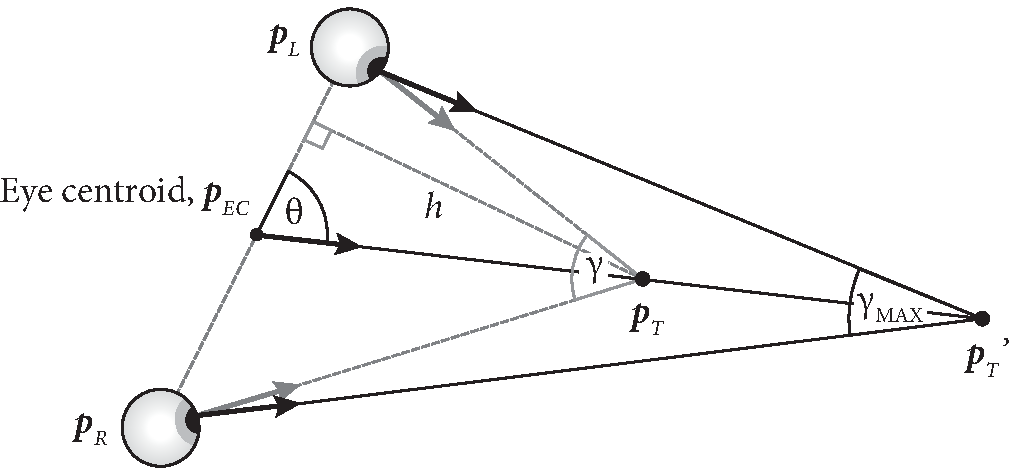
\includegraphics[width=0.85\textwidth]{stylizedgaze/Figures/CrosseyednessRemoval.pdf}
\caption{Our approach for reducing cross-eyedness in the target gaze pose.}
\label{fig:CrosseyednessRemoval}
\end{figure}

Our approach to remove cross-eyedness is illustrated in Figure~\ref{fig:CrosseyednessRemoval}. We measure cross-eyedness as the angle between the gaze directions of the two eyes, $\gamma$. Allowable cross-eyedness is defined by a threshold $\gamma_{MAX}$, which we leave at a default value of 0.002$^{\circ}$ for the examples in this paper.
We define the \textit{effective target position}, $\mathbf{p}_T'$, as the position behind the physical gaze target that the eyes can converge on without violating the cross-eyedness threshold. It is calculated by moving the target position away from the character to reduce $\gamma$ below the threshold value $\gamma_{MAX}$:

\begin{align}
\mathbf{p}_T' = \mathbf{p}_{EC} + \frac{\mathbf{p}_T - \mathbf{p}_{EC}}{||\mathbf{p}_T - \mathbf{p}_{EC}||} \frac{\sin(\theta + \gamma_{MAX}/2)}{sin(\gamma_{MAX}/2)}||\mathbf{p}_L - \mathbf{p}_{EC}||.
\end{align}

The above technique is effective at reducing cross-eyedness as shown in Figure~\ref{fig:CrosseyednessFixExample}.

The cross-eyedness removal technique is applied in a view-dependent manner; we may only apply it if the viewer cannot notice it from the current viewpoint.
If the viewer \emph{is} the gaze target, they may notice the character is looking a bit ``past'' them if cross-eyedness removal is applied.
Therefore, the cross-eyedness threshold $\gamma_{MAX}$ is adjusted based on the target viewing angle $\phi_T$, which we define as the angle between the viewer's gaze direction and the character's gaze direction at the target pose. We adjust $\gamma_{MAX}$ as follows:

\begin{align}
\label{eq:CrosseyednessFix}
\gamma\,'_{MAX} &= 2 OMR_{IN} + (\gamma_{MAX} - 2 OMR_{IN}) p_{\phi} \\
p_{\phi} &= \frac{\phi_T}{9.6W},~ 0 \le p_{\phi} \le 1 \nonumber
\end{align}

where $OMR_{IN}$ is inward OMR of the eye, and $W$ is the eye width parameter. The $9.6^{\circ}$ constant is derived from parameters of the viewing cone in which humans are able to detect subtle differences in gaze direction~\cite{argyle1976gaze}. We scale this value by $W$, as larger eyes may make such judgements easier. The viewing cone parameter, $p_{\phi}$, expresses the drop-off in judgement accuracy from the center of the cone toward the edge. We use $p_{\phi}$ to vary allowable cross-eyedness from the mechanical limit, $2 OMR_{IN}$, at the center of the cone, to $\gamma_{MAX}$ at the cone's edge and beyond.

\subsubsection{Eye Divergence}

\begin{figure}
\centering
\includegraphics[width=0.9\textwidth]{stylizedgaze/Figures/EyeDivergenceFixExample-small.pdf}
\caption{Example of eye divergence handling. Top: The VOR begins to move the left eye immediately on alignment. Bottom: Our model ensures that VOR begins eye movement only after the right eye has aligned.}
\label{fig:EyeDivergenceFixExample}
\end{figure}

A consequence of OMR asymmetry, eye divergence is handled by allowing the eyes to diverge during the gaze shift and imposing the principle that VOR for both eyes must trigger \emph{at the same time}. The leading eye will always overshoot the gaze target by a small amount and only begin moving in the opposite direction (due to VOR) when the trailing eye has reached the target. This behavior prevents the leading eye from aligning exactly with the target, as the accumulated overshoot rotation introduces an offset into the eye's target rotation. However, much like with cross-eyedness removal, this minor deviation from correct gaze convergence is difficult to detect. This technique is therefore an effective way of eliminating disconjugate eye movements as shown in Figure~\ref{fig:EyeDivergenceFixExample}.

As with cross-eyedness removal, eye divergence is applied in a view-dependent manner. The target overshoot introduced by the technique may be noticeable to the viewer at very low viewing angles, which we therefore adjust using the viewing cone parameter, $p_{\phi}$, that we defined in Equation~\ref{eq:CrosseyednessFix}. Specifically, we scale the outward OMR based on target viewing angle, $\phi_T$:

\begin{equation}
OMR_{OUT}' = OMR_{IN} + (OMR_{OUT} - OMR_{IN}) p_{\phi}
\end{equation}

This adjustment ensures that outward OMR will contract at low $\phi_T$, making the OMR symmetrical.

\subsection{Gaze Kinematics Adaptation}

\begin{figure*}
\centering
\includegraphics[width=1\textwidth]{stylizedgaze/Figures/GazeDynamicsExample1-small.pdf}
\caption{Gaze shifts with different gaze kinematics. Top: Original motion. The gaze shift contains the artifacts stuck eye, OMR-block, and eye retraction. Bottom: Our method. The artifacts of the original motion are reduced.}
\label{fig:GazeDynamicsExample}
\end{figure*}

Because most stylized characters do not have the same proportions and OMR as humans, we introduce a method for adapting the gaze shift kinematics based on these differences. The adaptation takes the form of scaling the gaze shift velocity. For our gaze shift model (Chapter~\ref{cha:GazeShiftModel}), that means changing the manner in which the peak eye velocity, $v_{\mathrm{max},E}$, is computed. However, the same adaptation can be applied to any gaze shift synthesis model that allows control over timing.

Our gaze kinematics adaptation is based on two key ideas. First, since stylized eyes can be asymmetric, each eye may need to cover a different angular distance as it rotates toward its OMR. We want to ensure that both eyes reach the OMR at the same time, thereby preventing artifacts such as \emph{stuck eye}. It follows that the eyes need to move at different velocities to reach the OMR at the same time. We define separate peak velocities, $v_{MAX,j}$, for each eye $j$. The second key idea is that stylized eyes are larger and therefore more massive than real human eyes, so they should move more slowly.

We use the anatomic parameters eye width, $W$, and muscle strength, $F$, to compute the peak eye velocities. As volume---and therefore mass---increases with $W^3$, both peak velocities are scaled down by the same factor. $F$ is used to compute an intermediate parameter $F'$, which varies depending on how much the head contributes to the gaze shift. We compute $F'$ as follows:

\begin{equation}
F' = ( 1 - \alpha_H ) W^3 + \alpha_H F.
\end{equation}

The parameter $\alpha_H$ specifies how much the head contributes to the gaze shift. When the head carries the eyes through most of the gaze shift (high $\alpha_H$), eye velocity should be lower in order to prevent the eyes from appearing improbably fast. When the head moves only a small distance, the eyes should move more quickly to prevent the gaze shift from appearing slow and sluggish.

To account for OMR asymmetry and prevent artifacts such as \textit{stuck eye}, we also need to apply a separate scaling factor to each velocity. Assume that $A_{OMR,j}$ is the distance that the eye $j$ can rotate before reaching its OMR, while $A_{MAX}$ is the highest rotational distance to the OMR for \emph{both} eyes. The peak velocity is scaled by $A_{OMR,j}/A_{MAX}$. This has the effect of slowing down the eye that has less rotation to complete, thus ensuring that both eyes reach the OMR at the same time.

Finally, we also introduce a velocity multiplier parameter, $\chi$, and apply it uniformly to eye and head velocities. This parameter can be used to make the character's gaze appear livelier or more languid, depending on their size, personality, and mood. By default, $\chi$ is set to $1$, although we use values between $1.2$ and $1.7$ for our stylized characters.
% NOTE: Clarified how the parameter might be used by explaining how we use it. -- Tomislav

We introduce these modifications to Equation~\ref{eq:AndristVmaxE} to create the following updated equation for calculating peak eye velocities:

\begin{equation}
v_{MAX,j} = \frac{F}{W^3}( \frac{2}{75} A_{MAX} + \frac{1}{6} ) \frac{A_{OMR}}{A_{MAX}} \chi v_0%+ 3 \delta V_{MAX,H}
\end{equation}

The first, third, and fourth terms implement our modifications to gaze kinematics. The second term speeds up or slows down the eyes depending on eye movement amplitude and is similar to the term used by the original model to calculate the peak velocity, except that $A_{MIN}$ is replaced by $A_{MAX}$.
%The rightmost term $3 \delta v_{MAX,H}$ addresses an issue with the original gaze model. For certain rare gaze shifts, the angle $\delta$ between eye and head rotation directions may become much greater than 0; eyes could even end up moving in the opposite direction of the head. In these cases, the head is slowing down the eyes rather than helping them reach the target, so the above term speeds up the eyes to compensate for the opposing head rotation.
% Since this is a bugfix of the original model, maybe it doesn't need to be here? It muddles the story somewhat, and takes up space...

Using the above method for calculating peak eye velocities reduces the artifacts related to gaze kinematics, producing gaze shifts that appear smoother and more lifelike. The stuck eye artifact is largely eliminated; the amount of time spent in the state of OMR-block is greatly reduced; and the VOR causes less eye retraction (Figure~\ref{fig:GazeDynamicsExample}). The eye retraction cannot be completely eliminated, as some VOR must occur to achieve the specified head alignment and thus produce desired communicative effects.

\subsection{Gaze-evoked Eye Blinks}

\begin{figure}
\centering
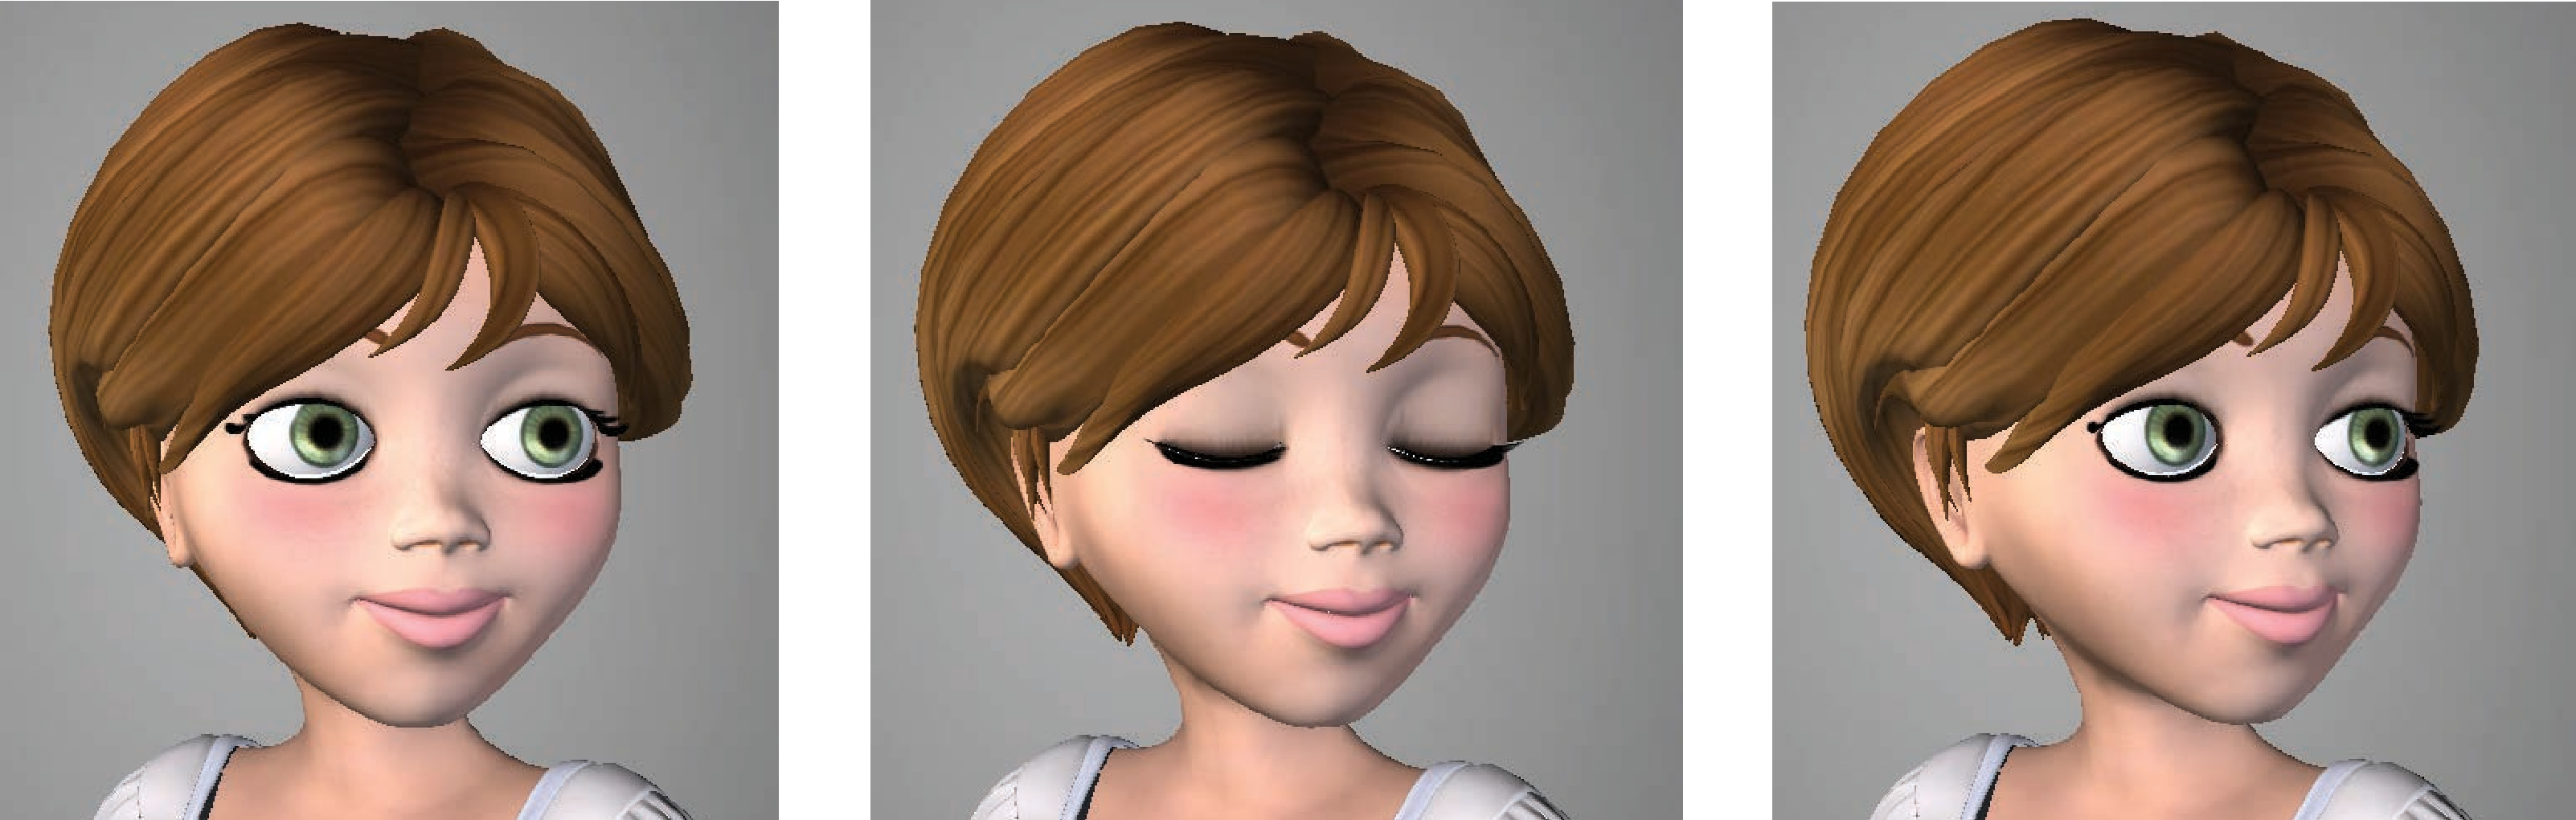
\includegraphics[width=0.85\textwidth]{stylizedgaze/Figures/GazeEvokedBlinkVOR-small.pdf}
\caption{A gaze-evoked eye blink during the VOR phase. The blink conceals the retraction in the left eye.}
\label{fig:GazeEvokedBlinkVOR}
\end{figure}

As described in Section~\ref{sec:GazeShiftSecondary}, our gaze shift model also incorporates gaze-evoked eye blinks. At the beginning of the gaze shift, it is probabilistically determined whether or not a gaze-evoked eye blink will occur.
The timing of the blink is deterministic---if generated, the blink occurs immediately at the start of the gaze shift.
As part of our efforts to reduce gaze animation artifacts, we propose introducing more variability into the timing of gaze-evoked blinks. Specifically, we schedule the blinks to co-occur with potential eye retraction artifacts in order to conceal them by the character's eyelids (Figure~\ref{fig:GazeEvokedBlinkVOR}).

Our implementation generates a gaze-evoked eye blink at the start of the gaze shift, using the same probabilistic method as in the baseline model. However, when determining the timing of the blink, we estimate the duration of the VOR phase of the gaze shift, $T_{VOR}$, and the time when the VOR phase will begin, $t_{VOR}$. If $T_{VOR}$ is greater than a threshold value, then the gaze-evoked blink is scheduled to begin at $t_{VOR} - 0.35T_{B}$, where $T_B$ is the duration of the eye blink (generated probabilistically), and $0.35T_B$ is the time when the eyes are fully closed.


\section{Performative Gaze}
\label{sec:PerformativeGaze}
\begin{figure}
\centering
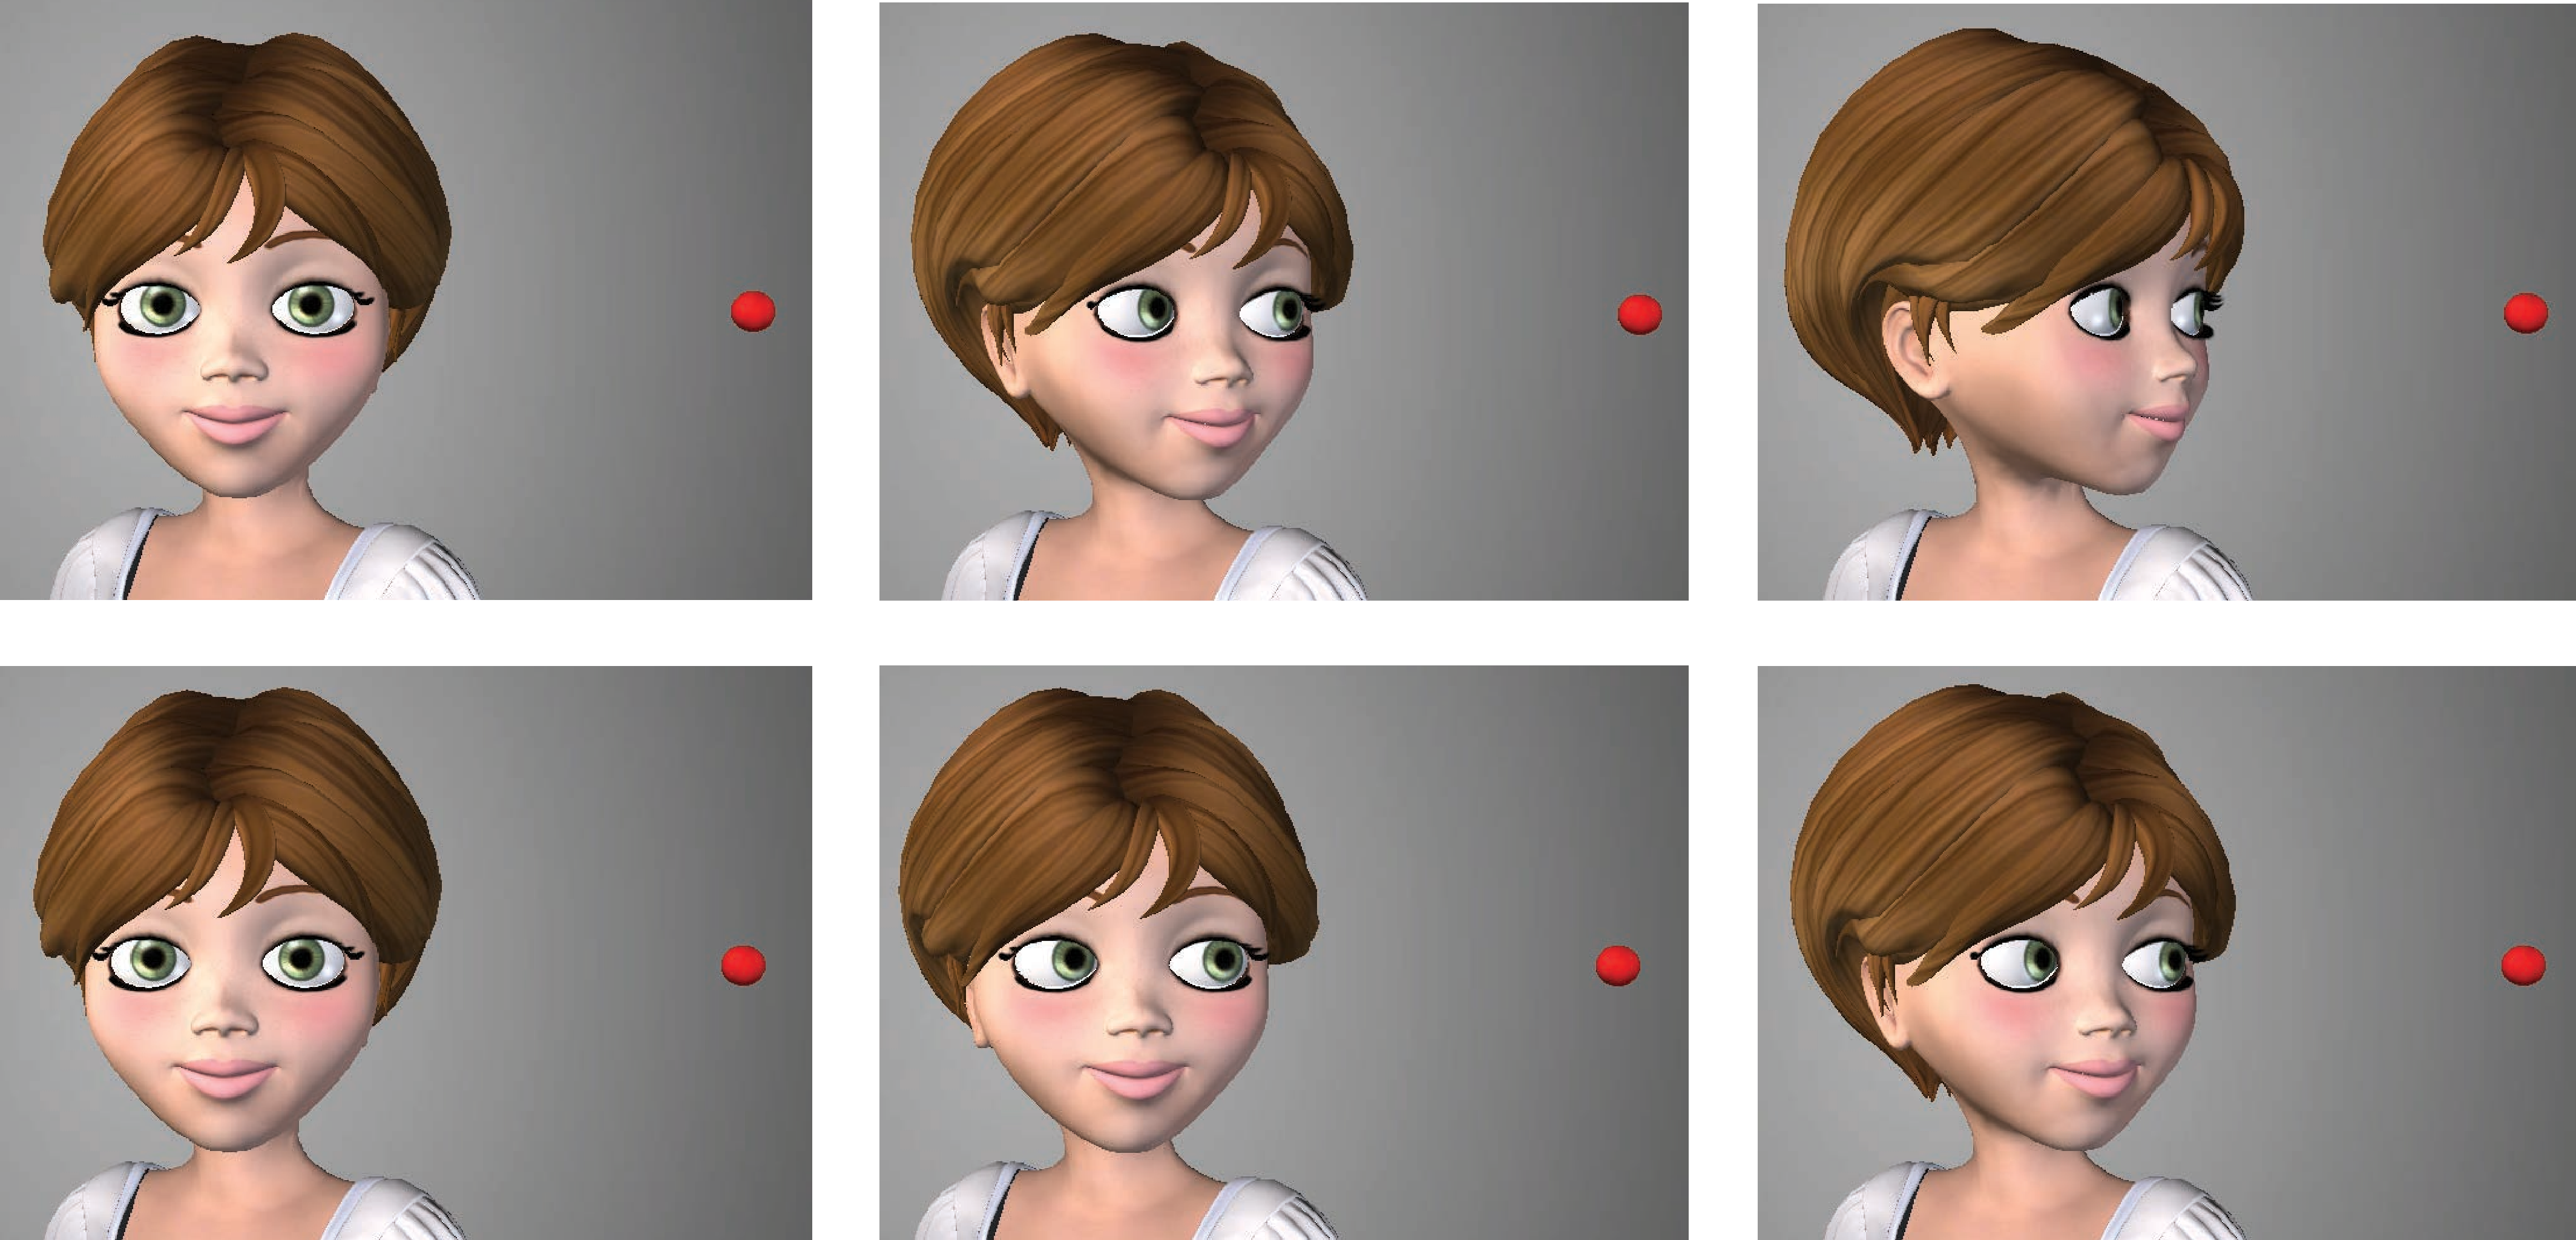
\includegraphics[width=0.9\textwidth]{stylizedgaze/Figures/PerformativeGazeExample-small.pdf}
\caption{A performative gaze shift. Top: The character fully aligns its gaze with the red sphere. Bottom: The character partially aligns its gaze with the target ($\alpha_E = 0.7$) but still appears to be gazing at it, because it has achieved screen-space alignment.}
\label{fig:PerformativeGazeExample}
\end{figure}

\begin{figure}
\centering
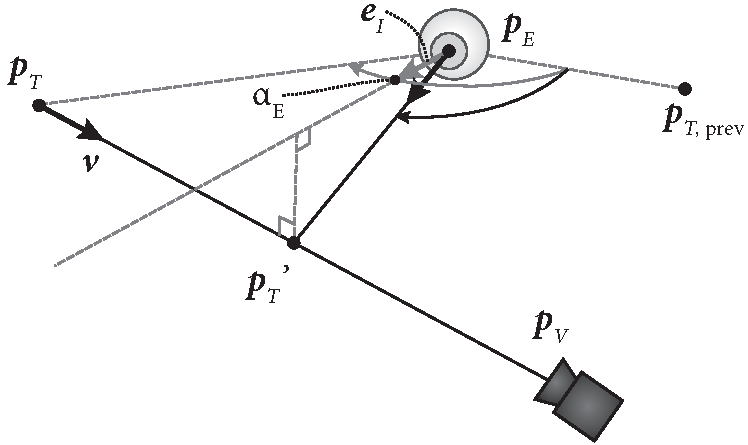
\includegraphics[width=0.75\textwidth]{stylizedgaze/Figures/EyeAlignment.pdf}
\caption{The calculation of the effective gaze target position in a performative gaze shift.}
\label{fig:EyeAlignment}
\end{figure}

While humans use gaze to seek information from their environment, in acting and cartoon animation, the primary purpose of gaze is to communicate ideas to and creating engagement with an audience. These goals can be achieved by performing partial gaze shifts in the general direction of the object of interest in order to convey the idea that the character is attending to the object without precisely aligning gaze with it. This performative behavior allows the character to retain partial alignment with the audience, enabling them to better see what the character is doing and making the character's performance more immediate and engaging. The notion that viewers prefer it when a virtual character or real person faces them more is strongly supported by research, e.g.,~\citep{beebe1976effects,andrist2012designing}.

We introduce a motion adaptation method for gaze shifts that allows the synthesis of performative gaze shifts. The method exposes an eye alignment parameter, $\alpha_E$, which allows the animator to specify the desired amount of alignment with the target. Setting $\alpha_E = 1$ causes the eyes to fully align with the target.
% NOTE: More detailed explanation of how the parameter can be tweaked -- Tomislav
With parameter values lower than $1$, the character will gaze toward a point directly between the gaze target and the viewer, which we call the \textit{effective gaze target}. In order to convince the viewer that the character is gazing toward the real target, the two targets must line up in the screen space, as illustrated in Figure~\ref{fig:PerformativeGazeExample}.

Figure~\ref{fig:EyeAlignment} illustrates how the specified eye alignment is achieved. We compute the intermediate rotation of each eye using $\mathbf{q}_I = slerp (\mathbf{q}_S, \mathbf{q}_T, \alpha_E )$, where $\mathbf{q}_S$ and $\mathbf{q}_T$ are the eye orientations in the source and target pose, respectively. At this orientation, the eye's gaze direction is given by the ray $\mathbf{e}_I$. The view direction ray, $\mathbf{v}$, points from the target position $\mathbf{p}_T$ to the viewer. Effective gaze target position, $\mathbf{p}_T'$, is the point along the ray $\mathbf{v}$ that is the closest to the ray $\mathbf{e_I}$.

Similar to the target pose adaptation techniques described in Section~\ref{sec:StylizedGazeTargetPoseAdaptation}, partial eye alignment is applied in a view-dependent manner. At low target viewing angles, $\phi_T$, the method enforces full eye alignment to prevent the viewer from noticing that the character is not actually gazing at them by automatically adjusting it using the viewing cone parameter, $p_{\phi}$, as follows:
%
\begin{equation}
\alpha_E' = 1 - p_{\phi} + \alpha_E p_{\phi}.
\end{equation} 

\section{Evaluation}
\label{sec:StylizedGazeEvaluation}
This section presents two forms of evaluations of our gaze model. The first evaluation involved an \textit{objective} assessment of the effectiveness of our model in reducing the frequency and severity of visual artifacts in gaze shifts on different character designs. The second evaluation followed a human-subjects study and assessed the \textit{perceived} characteristics of the generated gaze behaviors.

\subsection{Objective Evaluation}

To evaluate the effectiveness of our model in reducing visual artifacts, we have conducted measurements of artifact prevalence on a variety of characters using a set of objective metrics. These metrics reflected the amount of observable artifacts over the course of a gaze shift. Because each artifact is a product of a particular combination of the pose and movement of the eyes and the head, whether or not the artifact is present at a particular frame and its severity can be objectively determined and quantified. Each metric computes the presence of an artifact in each frame and sums them over all the frames of the gaze shift to calculate the ``amount'' in which the artifact appears. Severity is determined by weighing the amount of an artifact by the cosine fall-off of the viewing angle, $\phi$ (i.e., angle between view direction and character's gaze direction), thus giving less weight to frames where the character's eyes are less visible. The artifact amount is also weighed by the blink height at each frame to account for eye blinks that partially or fully conceal artifacts. The aggregated amounts are then normalized by the duration of the gaze shift, providing us with quantities that we can compare across different characters and gaze shift configurations. Our metrics include cross-eyedness amount, $\tau_{CE}$, OMR-block amount, $\tau_{OMR}$, eye retraction and divergence amount, $\tau_{ERD}$, and stuck eye amount, $\tau_{SE}$.
% NOTE: removed redundant explanations of metrics -- Tomislav

% See http://www.inf.ethz.ch/personal/markusp/teaching/guides/guide-tables.pdf for info on making nice tables
\begin{table}[b!]
\footnotesize
\centering
\caption{Quantitative evaluation results. Each cell contains the aggregate score for a particular metric on a particular character with the baseline model or our proposed model.}
\vspace{4pt}
\begin{tabular}{@{}llcccc@{}}\toprule
Character & Model & $\tau_{CE}$ & $\tau_{OMR}$ & $\tau_{ERD}$ & $\tau_{SE}$ \\
\midrule
RealisticFemale1 & \textbf{Baseline} & 0.30 & 0.24 & 0.20 & 0.03 \\\hdashline
RealisticFemale2 & \textbf{Baseline} & 0.31 & 0.22 & 0.20 & 0.03 \\\hdashline
\multirow{2}{*}{SemiStylizedFemale} & \textbf{Baseline} & 0.31 & 0.23 & 0.18 & 0.03 \\
& \textbf{Proposed} & 0.07 & 0.10 & 0.10 & 0.02 \\\hdashline
\multirow{2}{*}{StylizedFemale} & \textbf{Baseline} & 0.40 & 0.25 & 0.21 & 0.05 \\
& \textbf{Proposed} & 0.12 & 0.10 & 0.10 & 0.02 \\\hdashline
\multirow{2}{*}{StylizedMale} & \textbf{Baseline} & 0.32 & 0.22 & 0.17 & 0.03 \\
& \textbf{Proposed} & 0.09 & 0.10 & 0.10 & 0.03 \\\hdashline
\multirow{2}{*}{EmotiGuy} & \textbf{Baseline} & 0.27 & 0.33 & 0.20 & 0.07 \\
& \textbf{Proposed} & 0.06 & 0.12 & 0.13 & 0.03 \\\hdashline
\multirow{2}{*}{Jack} & \textbf{Baseline} & 0.06 & 0.46 & 0.11 & 0.05 \\
& \textbf{Proposed} & 0.07 & 0.16 & 0.07 & 0.06 \\\hdashline
\multirow{2}{*}{Donkey} & \textbf{Baseline} & 0.18 & 0.34 & 0.22 & 0.10 \\
& \textbf{Proposed} & 0.04 & 0.10 & 0.15 & 0.03 \\\hdashline
\multirow{2}{*}{Fish} & \textbf{Baseline} & 0.54 & 0.30 & 0.26 & 0.08 \\
& \textbf{Proposed} & 0.16 & 0.10 & 0.14 & 0.03 \\\hdashline
\multirow{2}{*}{NastyMonster} & \textbf{Baseline} & 0 & 0.20 & 0.29 & 0 \\
& \textbf{Proposed} & 0 & 0.09 & 0.18 & 0 \\
\bottomrule
\end{tabular}
\label{tab:EvalResults}
\end{table}

For our test cases, we generated $138$ random gaze shifts and applied them to ten different characters, including two with realistic, humanlike proportions (Figure~\ref{fig:TestCases}). The gaze shifts included an even number of shifts with full and minimal head alignment. For each character, we aggregated the measurements for all gaze shifts with the same head alignment. The results show a reduction in artifact prevalence in almost all test cases as summarized in Table~\ref{tab:EvalResults} and below:

\begin{itemize}

\item Cross-eyedness, $\tau_{CE}$, in characters with human proportions has an average value of $0.30$ and goes up to $0.54$ in characters with larger inter-eye distances. These levels of cross-eyedness cause unacceptable visual artifacts in stylized characters with large eyes, which are significantly reduced by our model.

\item $\tau_{OMR}$ is $0.22$--$0.24$ for realistic characters and can be as high as $0.46$ in stylized characters with very narrow OMR such as Jack. Our model reduces it by $30$--$60$\%, bringing it to about half of normal human levels and achieving a slower movement toward OMR in larger eyes.

\item $\tau_{ERD}$ is approximately $0.20$, $0.30$, and $0.10$ in realistic characters, characters with wide (e.g., NastyMonster) or highly asymmetric OMR (e.g., Fish), and characters with low OMR (e.g., Jack), respectively. Our model succeeds in reducing these values by $30$--$50$\%.

\item Even characters with human proportions exhibit a small amount of stuck eye, $\tau_{SE}$, which we believe is too small to notice. With characters with asymmetric OMR (e.g., EmotiGuy, Jack, Donkey, Fish), $\tau_{SE}$ can be as high as $0.10$. Our model reduces it to levels seen in human characters. An exception is the Jack character with very narrow OMR, which offers little flexibility in the movement.

\end{itemize}

\subsection{Human Subjects Study}

To lessen visual artifacts and afford staging effects, our model deliberately directs the characters's gaze shifts toward locations that are different from the intended gaze targets. While these shifts do not involve geometrically accurate gaze motions, previous studies on gaze perception have shown that people are generally imprecise at judging gaze direction \cite{argyle1976gaze}, suggesting that these deviations might not worsen judgments that already show very high variability. Therefore, the evaluation sought to determine whether these deviations affected the communicative accuracy and perceived naturalness of gaze shifts generated by our model compared with a previously validated baseline model \cite{andrist2012headeye}.

% TODO: Any information on participant profile?
\textit{Participants} -- We recruited 48 participants using the Amazon Mechanical Turk crowd-sourcing service. Each participant was paid U.S. \$1 for their participation.

\textit{Study Design} -- The study followed a three-by-one, between-participants design. The experimental conditions included gaze shifts performed by (1) \textit{baseline}: a character with human proportions following the baseline gaze model, (2) \textit{baseline stylized}: a character with stylized geometry following the baseline gaze model, and (3) \textit{stylized}: a character with stylized geometry following our gaze model. We chose a between-participants design to minimize transfer effects. Figure~\ref{fig:StudyTask} illustrates the two characters used in the study. The \textit{stylized} condition involved performative gaze shifts with an eye-alignment parameter of $0.85$.

\begin{figure}[t]
\centering
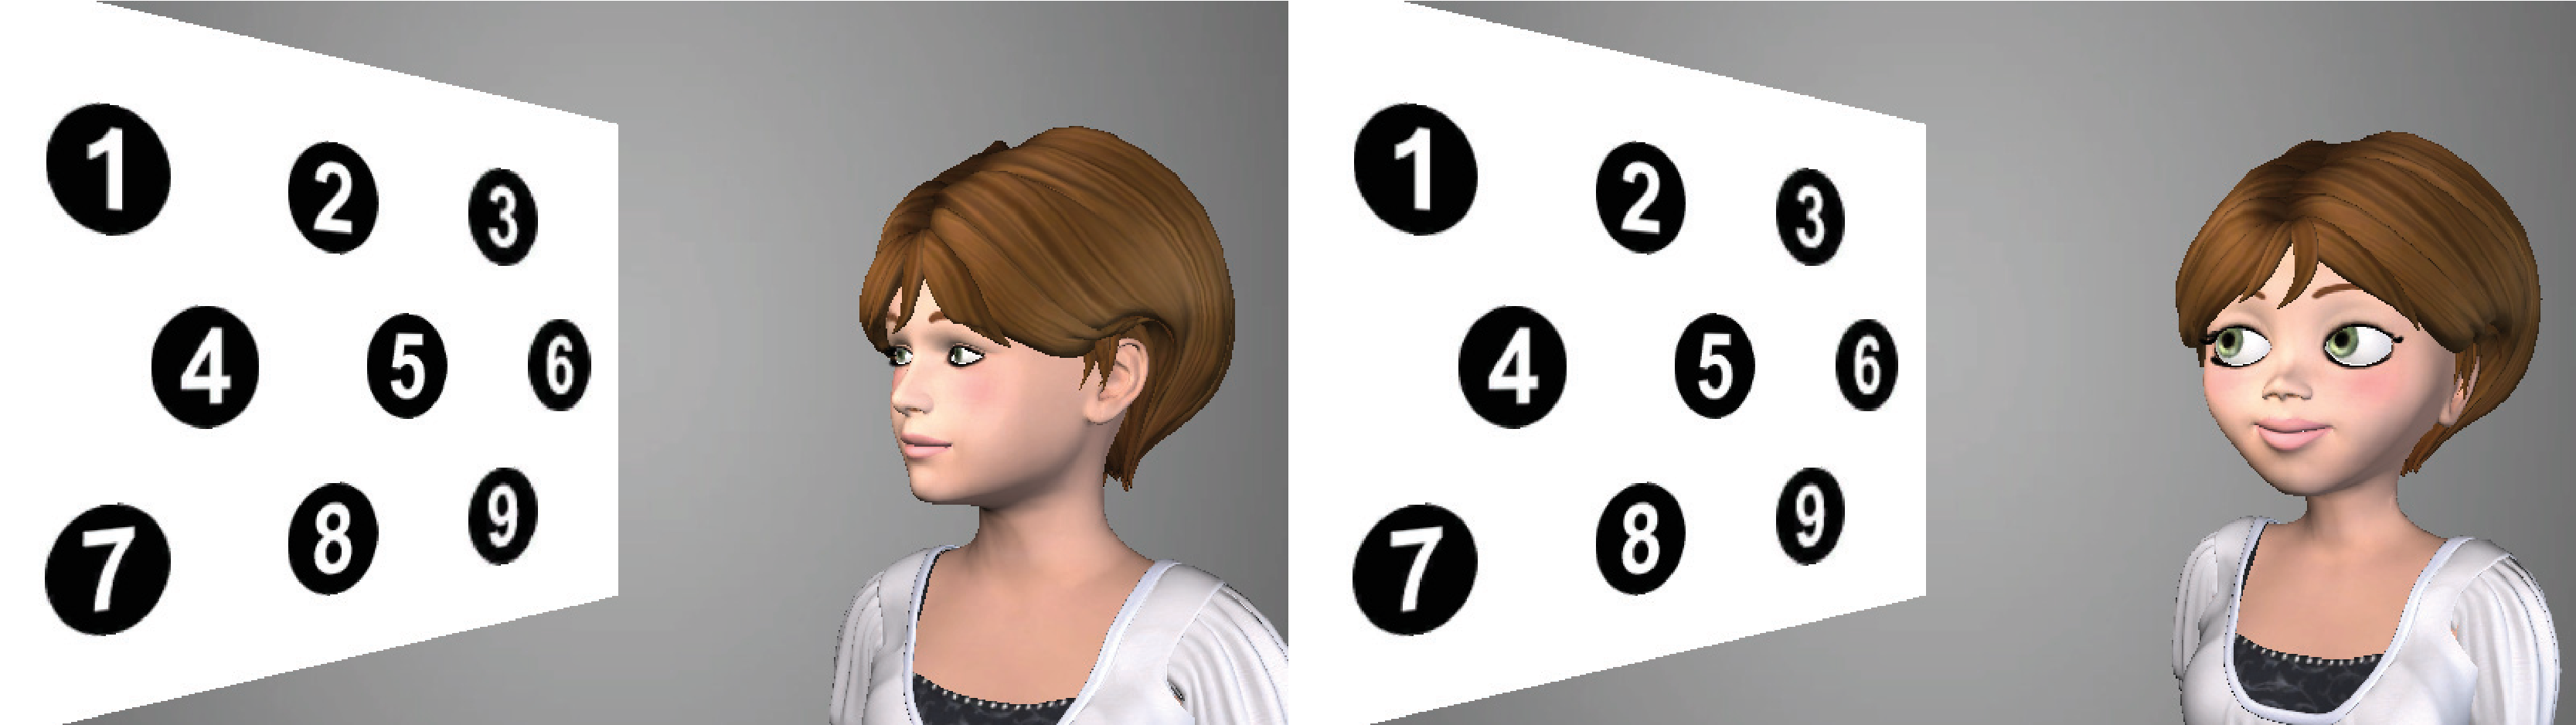
\includegraphics[width=0.48\textwidth]{Figures/StudyTask-small.pdf}
\caption{Stills from videos in our study. Left: Realistically-proportioned character. Right: Stylized character.}
\vspace{-12pt}
\label{fig:StudyTask}
\end{figure}

\textit{Task} -- Participants in the study watched a series of videos of the character shifting its gaze toward numbered targets arranged on a whiteboard and tried to identify the target toward which the character was looking (Figure~\ref{fig:StudyTask}). The character was positioned in front of the camera, approximately $1 m$/$3.3 ft$ away and slightly to the right. The whiteboard was positioned on the character's right and oriented so that the viewer and the character could comfortably see the targets.

\textit{Procedure} -- After recruitment, each participant reviewed and agreed to a consent form. Following informed consent, the participants viewed a sequence of $22$ videos. In each video, the character shifted its gaze toward a randomly selected target from among nine targets on the whiteboard. After watching each video, the participants were asked to determine the target toward which the character was looking and provide their answer in a text field. Each video was approximately ten seconds in length. At the beginning of each video, the character looked toward the camera and nodded. It then shifted its gaze toward one of the targets, maintained its gaze at the target for two seconds, and then looked back toward the viewer.

To ensure the quality of the experimental data, we followed crowd-sourcing best practices \cite{kittur2008mturk}. For example, all participants were shown two training and acclimation videos, where    the correct gaze target would light up during the gaze shift. Data from participants who failed to correctly identify the target were discarded. We also restricted the task to workers with high approval rates and tracked statistics such as task completion time and screen resolution.
% NOTE: Explained our quality control procedure in more detail. -- Tomislav

At the end of the study, each participant filled out a questionnaire to provide subjective evaluations of the character. The study took approximately ten minutes.

\begin{figure}[!b]
\centering
\vspace{-8pt}
\includegraphics[width=0.48\textwidth]{Figures/Results.pdf}
\caption{Results for communicative accuracy, lifelikeness, appeal, and naturalness of eye movements. Data on gaze shifts generated by our model are shown in red.}
\vspace{-8pt}
\label{fig:StudyResults}
\end{figure}

\textit{Measurement \& Analysis} -- The dependent variables in our study were \textit{communicative accuracy}, \textit{naturalness of eye movements}, \textit{lifelikeness}, and \textit{appeal}. Communicative accuracy was measured as the percentage of correctly identified gaze targets. Naturalness of eye movements, lifelikeness, and appeal were measured using a questionnaire. Participants rated each item in the questionnaire using seven-point rating scales ($1 = not likable$; $7 = likable$). The lifelikeness scale included three items that measured lifelikeness, humanlikeness, and believability ($Cronbach's \alpha = 0.799$), while the appeal scale included four items that measured charisma, attractiveness, cuteness, and likability ($Cronbach's \alpha = .796$).

Data analysis included one-way analysis of variance (ANOVA) tests, following guidelines suggested by Julnes and Mohr \cite{julnes1989analysis} for establishing a ``no difference'' in comparisons, particularly an alpha level of $0.25$ (i.e., $p > .25$) to control for Type II errors.
%http://deepblue.lib.umich.edu/bitstream/2027.42/67182/2/10.1177_0193841X8901300604.pdf

\textit{Results} -- Results for all measures are illustrated in Figure \ref{fig:StudyResults}. The mean accuracies in the baseline, baseline stylized, and stylized conditions were $54.0\%$, $58.6\%$, and $54.0\%$, respectively. The statistical analysis of the data found no significant effect of our manipulation on accuracy, $F(2,45) = 0.83$, $p = 0.44$. These rates are considerably better than chance, which we expect to be closer to 1/3 than 1/9, as our informal analysis suggests that it is easy to determine toward which row is being looked, and are consistent with results from previous work \cite{argyle1976gaze,goldberg1969distance,andrist2012designing}. Pairwise contrast tests also found no differences between the baseline and baseline stylized conditions, $F(1,45) = 0.00$, $p = 1.00$, or between the baseline and stylized conditions, $F(1,45) = 1.20$, $p = 0.28$. These results suggest that our model retains the communicative accuracy of the baseline human model.

Our analysis revealed no significant effect of our manipulation on naturalness of eye movements, $F(2,45) = 1.27$, $p = 0.29$. Contrast tests also found no differences between the baseline and baseline stylized conditions, $F(1,45) = 0.53$, $p = 0.47$, or between the baseline and stylized conditions, $F(1,45) = 2.52$, $p = 0.12$, suggesting that our model preserves the naturalness of eye movements generated by the baseline model.

We found no significant effects of our manipulation on the lifelikeness measure, $F(2,45) = 0.69$, $p = 0.51$. Pairwise contrasts showed no differences between the baseline and baseline stylized conditions, $F(1,45) = 0.10$, $p = 0.75$, or baseline stylized and stylized conditions, $F(1,45) = 0.64$, $p = 0.43$. Similarly, we found no effects of our manipulation on the appeal measure, $F(2,45) = 0.25$, $p = 0.78$. No differences appeared in pairwise contrast tests between the baseline and baseline stylized conditions, $F(1,45) = 0.18$, $p = 0.68$, or baseline stylized and stylized conditions, $F(1,45) = 0.49$, $p = 0.49$.

Overall, the results suggest that our gaze model does not change the communicative accuracy and the subjective evaluation of the characters. While we speculate that the removal of artifacts may improve a character's appeal, such effects are unlikely to appear in short, focused tasks. Future studies might further explore how our model shapes subjective impressions of the character in longer, more realistic scenarios.

\section{Discussion}
\label{sec:StylizedGazeDiscussion}
This chapter has described methods for adaptation of gaze shift motion that allow stylized characters to be animated using models for humanlike gaze shift synthesis. The methods work by adjusting the effective gaze target position and gaze shift kinematics to reduce distracting animation artifacts that would otherwise occur on stylized characters. The methods are demonstrated as extensions of the gaze shift model from Chapter~\ref{cha:GazeShiftModel}, though they can be used in conjunction with any gaze shift synthesis method that allows control over the target position and gaze shift timing.

Motion adaptations are applied in a view-dependent way and only allowed to deviate from biological constraints of human gaze when such deviations are undetectable to the viewer. The idea of adapting gaze motion in relation to the camera position in the scene is novel and we use it as a foundation of another method---performative gaze---which allows us to synthesize partially-aligned gaze shifts toward targets in the scene, while maintain the character's alignment---and involvement---with the audience. A study with human participants confirms that even though our methods depart from accurately representing human biological motion, the resulting gaze behavior is no less accurate than the original, humanlike gaze in communicating attention direction. On the other hand, our examples and objective measurements show that the proposed methods are effective in reducing animation artifacts across a range of character designs. Therefore, they contribute to the central objective of this dissertation, which is to facilitate the creation of communicatively effective gaze animation in a scalable way.



\chapterstyle{deposit}
\pagestyle{deposit}

\chapter{Gaze Animation Authoring}
\label{cha:GazeAuthoring}

\section{Introduction}
\label{sec:GazeAuthoringIntro}
Directed gaze is an important component of good character animation, as it can situate characters in the scene, signal the focus of their attention, and convey their personality and intent. Directed gaze involves coordinated movements of the eyes, head, and body. In animation practice, these movements are typically hand-authored, which requires considerable effort and skill due to their intricate spatial and timing relationships. Performance capture is seldom a viable option for obtaining high-quality gaze animation: while some performance capture rigs may record eye movements, the recorded gaze seldom matches the virtual scene and needs to be edited by hand or authored from scratch.

Chapter~\ref{cha:GazeShiftModel} has introduced methods for synthesis of directed gaze shifts as building blocks of effective gaze behaviors, while Chapter~\ref{cha:StylizedGaze} has introduced motion adaptation methods for gaze shifts, facilitating their application to characters with varied designs. The latter approach makes the process of creating character animation more scalable from the standpoint of character design, as it removes the need to re-author or re-implement gaze behaviors for characters that depart from realistic, humanlike design. In the current chapter, I focus on a different dimension of scalability---making the creation of gaze animation more scalable with respect to the scenario. The problem tackled this chapter can be stated as follows: given a non-interactive scenario, consisting of a virtual scene (a set of 3D objects) with one or more virtual characters engaging in activities encoded in their captured body motion, can we automatically add plausible gaze animation to the characters and facilitate its convenient editing by novices?

To solve this problem, we introduce an approach for adding directed gaze movements to characters animated using full-body motion capture, which uses an abstracted representation of gaze movements as its foundation. Specifically, we represent the gaze behavior as a sequence of \emph{gaze instances}, where each instance specifies a gaze shift toward a target in the scene. Our approach uses this representation to: (1) automatically \emph{infer} plausible gaze that matches the given body motion and scene layout, thus providing a starting point for editing; (2) afford convenient \emph{editing} controls allowing an animator to easily refine the gaze behavior; and (3) \emph{synthesize} biologically plausible gaze animation that expresses the author's intent. Two key properties of our model enable convenient editing. First, it abstracts details of gaze shift timing and pose, allowing an animator to specify \emph{when} and \emph{where} to look, while kinematics of eye, head, and body movements are synthesized automatically by the gaze shift model introduced in Chapter~\ref{cha:GazeShiftModel}. Second, it anchors the gaze animation in the virtual scene for easy spatial editing. Gaze targets serve as editing handles attached to virtual objects and characters; animators can move these around and synthesized gaze animation automatically adapts to the new spatial constraints.

\subsection{Approach Overview}

In the proposed approach, we model the gaze behavior as a temporal sequence of gaze shifts and fixations toward target locations in the scene. Each gaze shift is a coordinated movement of the eyes, head, and torso toward the target, followed by a gaze fixation of that target. We refer to every such gaze shift-fixation pair as a \emph{gaze instance} specifying the gaze shift start time, target location, and head and torso alignment with the target. Given a sequence of gaze instances, our system synthesizes the corresponding gaze movements and applies them to the body motion. A gaze instance sequence can also contain gaps, during which no gaze motion is applied to the character---we refer to such gaps as \emph{unconstrained gaze}.
While directed gaze does not include all human gaze movements---e.g., smooth pursuit, saccades, and conversational aversions---many are well-approximated, e.g., the numerous gaze aversions in the ChatWithFriend scene (Section~\ref{sec:GazeEditingResults}).

Our workflow has three main components: (1) inference, (2) synthesis, and (3) editing. The gaze inference model (Section~\ref{sec:GazeInference}) analyzes the captured body motion and the virtual scene, and it produces a set of editable gaze instances. The idea of gaze inference from body motion is that the motion implicitly contains the head and torso components of the actor's gaze, so by analyzing its kinematic properties we can infer an approximate reconstruction of the original gaze behavior. This reconstruction can be used to automatically add eye animation to the original motion. Moreover, it serves as a starting point for manual editing (Section~\ref{sec:GazeEditing}). We provide a graphical tool allowing animators to hand-edit the gaze instances, e.g., by changing the spatial layout of gaze targets, adjusting gaze instance timings, fine-tuning head and torso poses, and adding or removing gaze instances. Given an inferred and (potentially) edited set of gaze instances, the synthesis component (Section~\ref{sec:GazeSynthesis}) produces the final gaze animation.

\section{Gaze Inference}
\label{sec:GazeInference}
The gaze inference component of our approach analyzes the input body motion and virtual scene and constructs a model of gaze movements as a sequence of gaze instances. Each gaze instance is a tuple $G = (f_s, f_x, f_e, T, \alpha_{H}, \alpha_{T})$, where $f_s$, $f_x$, and $f_e$ are gaze shift start frame, fixation start frame, and fixation end frame, respectively, and $T$ is the gaze target. $\alpha_{H}$ and $\alpha_{T}$ are the head and  torso \emph{alignment} parameters, which specify head and torso orientation relative to the target and serve as inputs into the gaze shift model (Section~\ref{sec:GazeShiftModel}). Their advantage is that they enable facile control over head and body pose during gaze editing.

Gaze inference begins with a signal analysis of the body motion to detect individual gaze instances and infer their timings ($f_s$, $f_x$, and $f_e$). Next, we analyze the character's view of the scene at the end of each gaze shift and infer the most probable target $T$. Finally, we compute the alignment parameter values, $\alpha_{H}$ and $\alpha_{T}$, from the head and torso poses at the end of each gaze shift.

\subsection{Gaze Instance Inference}
\label{sec:GazeTimingInference}

Human gaze shifts follow a particular kinematic pattern (Section~\ref{sec:GazeShiftModel}). The eyes, head, and torso accelerate toward the gaze target, reach their peak velocities at the midpoint of the gaze shift, and decelerate as they align with the target, at which point the fixation. We detect gaze shifts by searching for this pattern in the body motion using a three-step approach. First, we search for clusters of maxima in angular acceleration signals of the head and torso joints, which correspond to significant gaze events (gaze shift beginnings and ends). \citet{coleman2008staggered} used a similar method to extract extreme poses from a general body motion. Each pair of adjacent gaze events defines a motion interval, which can be either a gaze shift or fixation. In the second step, we classify the motion intervals into gaze shifts and fixations. Third, for each gaze shift-fixation pair, we generate a gaze instance.

\begin{figure}
\centering
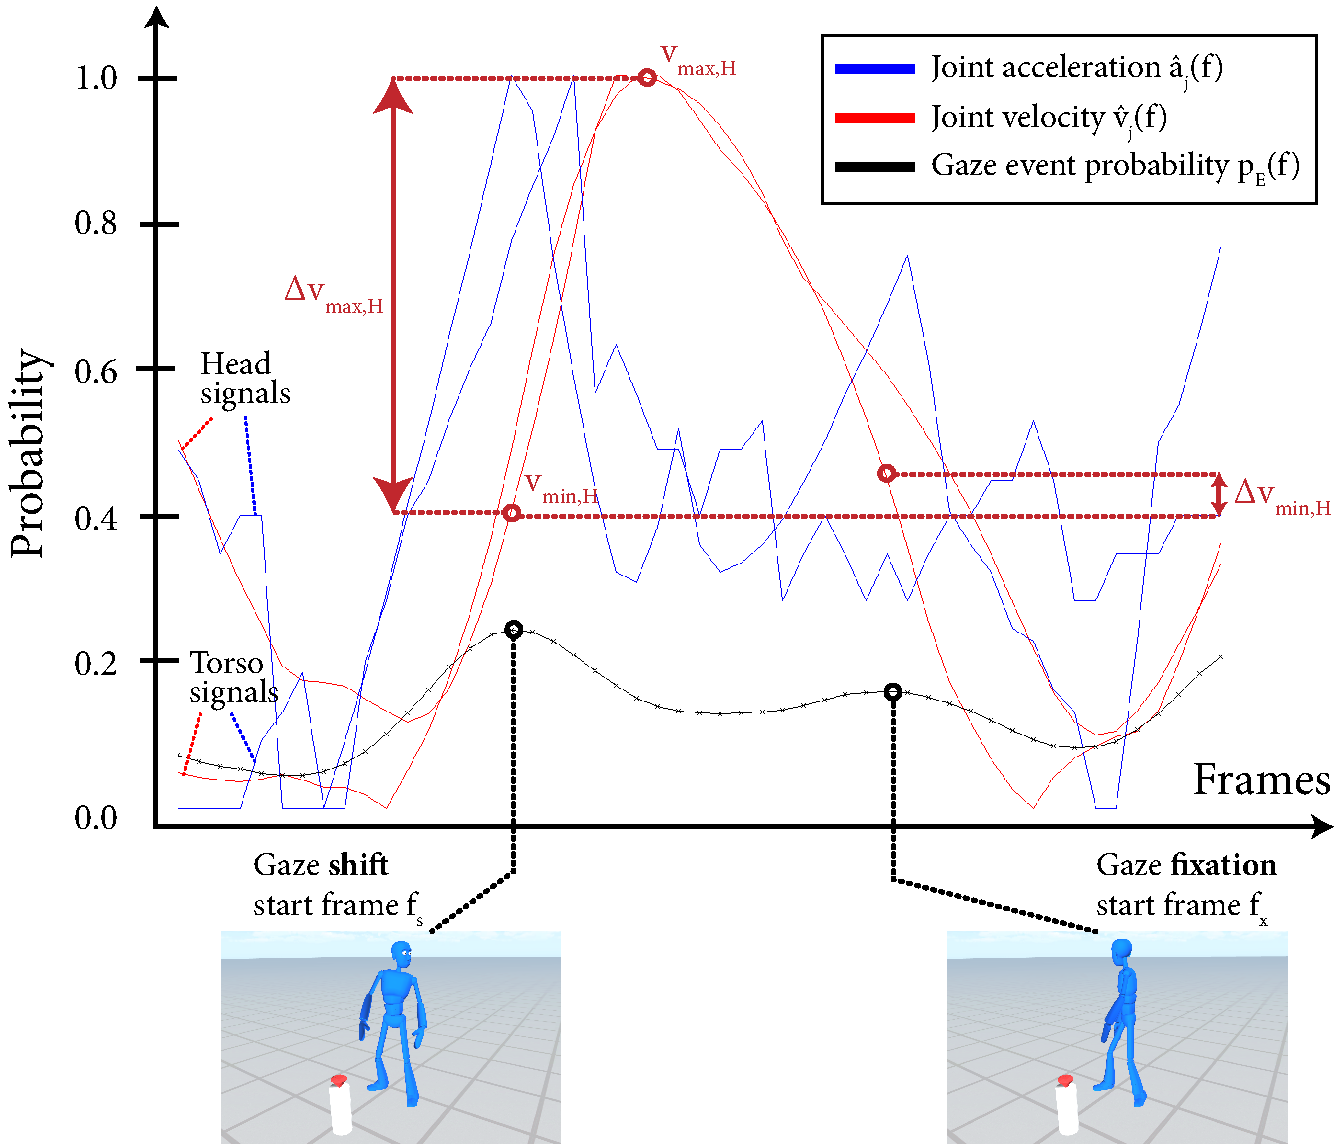
\includegraphics[width=0.9\textwidth]{gazeauthoring/Figures/GazeInstanceInference.pdf}
\caption{Gaze shift detection by analysis of acceleration and velocity signals of two joints---head and torso. We first aggregate the normalized joint accelerations $\hat{a}_j(f)$ into a global probability signal $p_E(f)$. Adjacent local maxima in $p_E(f)$ define the boundaries of a motion interval. We determine that the interval is a gaze shift from high peak joint velocity, $v_{\mathrm{max},j}$.}
\label{fig:GazeInstanceInference}
\end{figure}

\subsubsection{Gaze Event Discovery}

We discover gaze events by analyzing joint accelerations in the motion (Figure~\ref{fig:GazeInstanceInference}). Let $a_j(f)$ be the angular acceleration signal of joint $j$, defined across the motion's frame range ($f \in [0, L\rangle$, where $L$ is motion length in frames.) We normalize the acceleration signals to the 0-1 range: $\hat{a}_j(f) = a_j(f) / \mathop{max}(a_j(f))$. We use normalized acceleration signals of the root, torso, and head joints as local evidence measures indicating probability of significant gaze events (i.e, gaze shift starting or ending). We compute the global probability of a gaze event as a weighted sum of normalized acceleration signals:
%
\begin{align} \label{eq:GazeEventProbability}
p_E(f) = \frac{\sum_{j \in J} w_j \hat{a}_j(f)}{\sum_j w_j}
\end{align}
%
where $J$ is the set of joints, consisting of the root, torso, and head joints. Weights $w_j$ define each joint's influence on the global probability. We heuristically define a joint's weight to be greater the closer it is to the eyes, which means the head contributes more to the global probability than the torso or root. This choice is supported by findings (e.g.,~\citep{hietanen1999does}) showing the importance of head movements for the execution and perception of human gaze. We calculate joint weights as follows:
%
\begin{align} \label{eq:GazeJointWeight}
w_j(f) = \frac{1}{1 + l_j}
\end{align}
%
where $l_j$ is the distance of the joint $j$ to the eye joints, measured as cumulative length of the segments lying between them.

Local maxima in the probability signal, $p_E$, correspond to beginnings and ends of gaze shifts. Since acceleration signals are likely to be noisy and contain a large number of spurious maxima, a bilateral filter is applied to $p_E$, which smooths out the maxima resulting from noise and preserves those that are kinematically significant. We set the filter's range parameter $\sigma_r$ to 0.5 and spatial parameter $\sigma_s$ to 3. The filtered probability signal is then searched for local maxima. Each pair of adjacent maxima defines a motion interval $I_k = (f_{s,k}, f_{e,k})$, which could either be a gaze shift or a fixation.

\subsubsection{Motion Interval Classification}

To determine if a motion interval $I_k$ is a gaze shift, we use the fact that gaze shifts are characterized by peaks in joint velocity and we construct another probabilistic measure (Figure~\ref{fig:GazeInstanceInference}). Let $v_j(f)$ be the angular velocity signal of joint $j$. We define $v_{s,j}^k$ and $v_{e,j}^k$ to be joint velocities at the boundaries of interval $I_k$. Furthermore, let $v_{\mathrm{max},j}^k$ and $v_{\mathrm{min},j}^k$ be the maximum and minimum joint velocity over the interval $I_k$. Then we define maximum and minimum velocity differences as $\Delta v_{\mathrm{max},j}^k = v_{\mathrm{max},j}^k - \mathop{min} (v_{s,j}^k, v_{e,j}^k)$ and $\Delta v_{\mathrm{min},j}^k = \mathop{max} (v_{s,j}^k, v_{e,j}^k) - v_{\mathrm{min},j}^k$. Finally, we define the ratio of these quantities as follows:
%
\begin{align} \label{eq:GazeShiftRatio}
r_j^k =
\begin{cases}
0 & \text{if} \Delta v_{\mathrm{max},j}^k \leq 0 \\
\frac{\Delta v_{\mathrm{max},j}^k}{\Delta v_{\mathrm{min},j}^k} & \text{otherwise}
\end{cases}
\end{align}
%
Ratio $r_j^k$ increases with the peak velocity relative to the velocities at interval boundaries, suggesting that the interval is a gaze shift. We use a logistic function to map the ratio to a probability value in the 0-1 range:
%
\begin{align} \label{eq:GazeShiftProbability}
p_{S,j}^k = \frac{2}{1 + \mathop{exp}(-r_j^k)} - 1
\end{align}
%
Finally, we compute the gaze shift probability as a weighted sum of per-joint probabilities:
%
\begin{align} \label{eq:GazeShiftGlobalProbability}
p_S^k = \frac{\sum_{j \in J} w_j p_{S,j}^k}{\sum_j w_j}
\end{align}
%
where $w_j$ are the joint weights defined previously.

We classify the interval $I_k$ as a gaze shift if $p_S^k > P_{S,\mathrm{min}}$ (where $P_{S,\mathrm{min}}$ is a probability threshold set to 0.6 by default), otherwise we classify it as a fixation. Adjacent intervals that are classified as fixations get aggregated into a single fixation. We end up with a sequence of gaze shift-fixation pairs, from which we generate the sequence of gaze instances.

\subsubsection{Gaze Instance Generation}

For each gaze shift-fixation pair $(I_k, I_l)$, we generate a gaze instance $G = (f_s, f_x, f_e)$, such that the gaze shift starts at $f_s = f_{s,k}$, while the fixation starts at $f_x = f_{s,l}$, and ends at $f_e = \mathop{min}(f_{e,l}, f_{s,l} + L_\mathrm{max} - 1)$. Note that the fixation may not be longer than $L_\mathrm{max}$ (set to 1 second by default)---this is to prevent gaze from becoming ``stuck'' on a target for long periods of time.

Gaze shift probability threshold $P_\mathrm{min}$ is a useful parameter for controlling the density of gaze shifts found by the inference. Lowering the parameter to 0.5 results in subtle head and body movements being detected as gaze shifts and yields a more expressive behavior, albeit one that may be more challenging to edit---this setting was used for the ChatWithFriend example (~\ref{fig:GazeEditResults}, 5), which contains a lot of conversational gaze aversions. On the other hand, at parameter values above 0.6 only the most obvious gaze shifts are picked up, yielding a sparse gaze behavior that can be enriched further through manual editing.

\subsection{Gaze Target Inference}
\label{sec:GazeTargetInference}

In the preceding step, we inferred all the gaze instances and their timings. Next, for each gaze instance we infer its target in the scene. We assume there exists at least a simplified 3D model of the scene containing the key characters and objects, like those used for previsualization during film production. The result of gaze target inference is a sequence of gaze instances with associated targets. Gaze targets are handles in the scene attached to objects and other characters, which the animator can move around to change where the character is looking.

Our gaze inference method is based on three principles. First, the character is more likely to be looking at a point that lies along the movement direction of its head, as given in the body motion. If the character turns right, it is unlikely that the target lies to the left, up, or down. Second, the character is more likely to look at objects and other characters if they are \emph{important} to the story or task. For instance, in a scene where the character steals a gem, the gem is a likely gaze target. We allow the animator to manually label scene objects as important. Finally, the character is more likely to gaze at objects just before touching them or picking them up~\citep{johansson2001eyehead}. Assuming hand contacts are annotated in the body motion, we can easily get when a character is about to handle a scene object.

We propose a probabilistic approach to gaze target inference. Recall the gaze instance specification from the preceding step: $G = (f_s, f_x, f_e)$. $f_x$ is the gaze fixation start time, when we know the character's eyes are aligned with the gaze target, and therefore the target must be within the character's view. We compute a probability distribution, $p_T(\mathbf{x})$, over the 2D projection space representing the character's view of the scene at the frame $f_x$ ($\mathbf{x}$ being 2D projection coordinates). For each point in the character's view, $p_T(\mathbf{x})$ gives us the probability that the character is gazing at it. We find the gaze target $T$ at the global maximum of $p_T$.

We model $p_T(\mathbf{x})$ as a weighted sum of three probability terms, each implementing one principle of gaze target inference:
%
\begin{align} \label{eq:GazeTargetGlobalProbability}
p_T = \frac{w_d p_d + w_i p_i + w_h p_h}{w_d + w_i + w_h}
\end{align}
%
$p_d(\mathbf{x})$ is the directional term, which assigns higher probabilities to points lying along the head movement direction. $p_i(\mathbf{x})$ is the importance term, which is non-zero at points corresponding to objects and characters labeled as important. $p_h$ is the hand contact term, which is non-zero for objects that are about to be handled by the character (as indicated by hand contacts defined on the body motion). These terms contribute to the final probability, $p_T$, in proportion to their weights, $w_d$, $w_i$, and $w_h$. We find that the best inference results are obtained by setting these weights to 0.6, 0.15, and 0.25, respectively. Given the final probability $p_T$, we obtain the gaze target $T$ at the global maximum of $p_T$: $\mathbf{x}_T = \mathop{argmax}_{\mathbf{x}} p_T(\mathbf{x})$.

Figure~\ref{fig:GazeTargetInference} shows an example scene view with the associated probability distributions and gaze target location indicated. In the remainder of the section, we provide more detail about the computation of individual probability terms.

\begin{figure*}
\centering
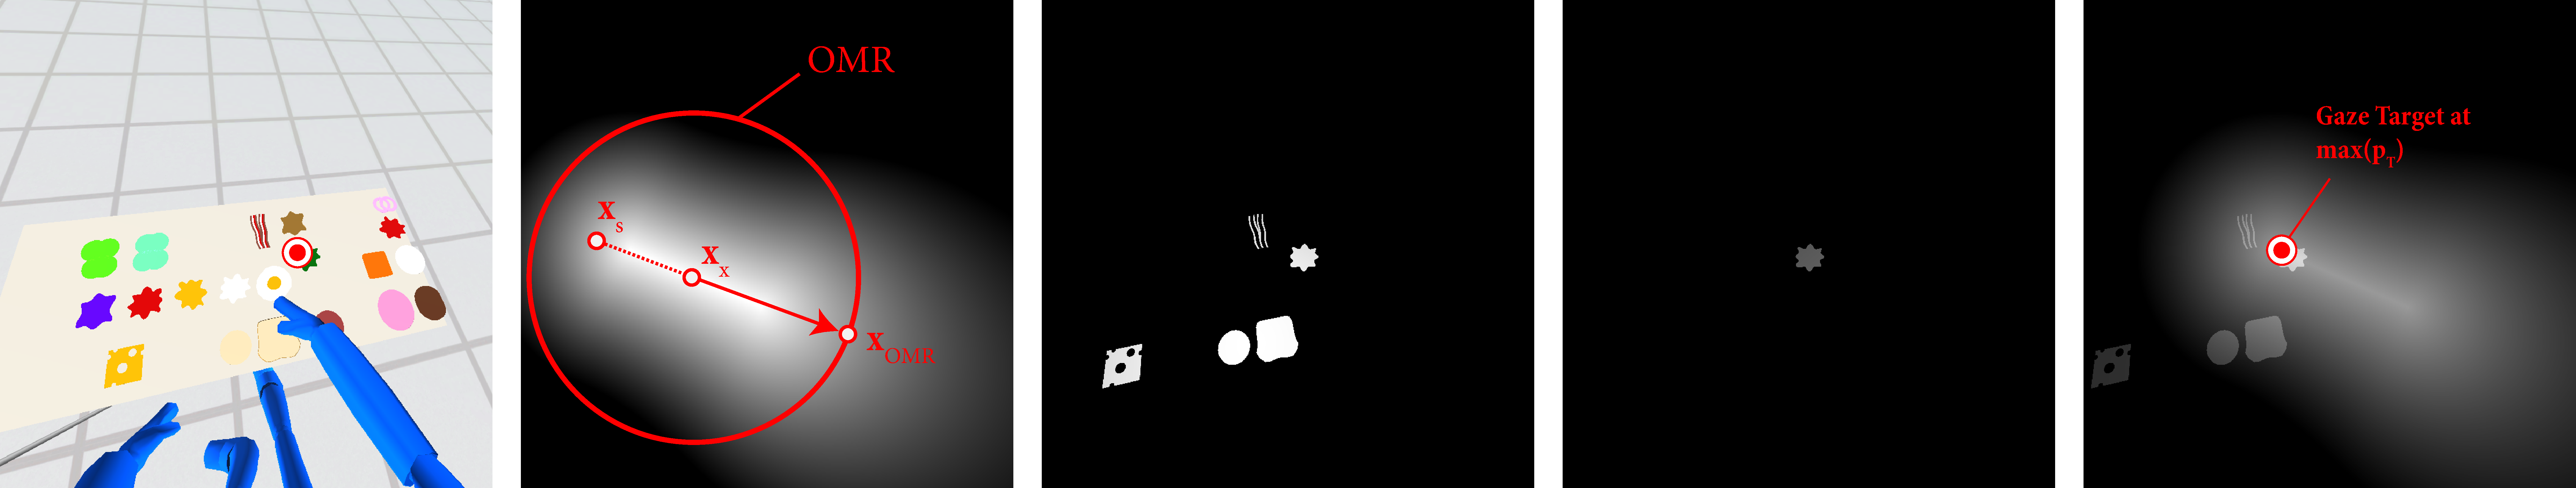
\includegraphics[width=1\textwidth]{gazeauthoring/Figures/GazeTargetInference.pdf}
\caption{We infer the gaze target by analyzing the character's scene view at the end of the gaze shift (1). The gaze target is more likely to lie along the head movement direction (directional term, 2), on an object labeled as important (importance term, 3), and on an object that is about to be touched or picked up (hand contact term, 4). We average these probability terms and find the gaze target at the global maximum (5).}
\label{fig:GazeTargetInference}
\end{figure*}

\subsubsection{Directional term}

Computation of the directional term, $p_d(\mathbf{x})$, is based on the following idea. When the character shifts its gaze, its head follows an approximately linear path in the projection space. Let us denote the start and end points of this path as $\mathbf{x}_s$ and $\mathbf{x}_x$ (Figure~\ref{fig:GazeTargetInference}b). If the character always gazed at things head-on, then $p_d(\mathbf{x})$ would be the highest at the end of the path, $\mathbf{x}_x$. However, the character is as likely to be looking at something out of the corner of the eye, so the eyes may ``overshoot'' $\mathbf{x}_x$ and line up with a point further along the movement direction. Therefore, from the path $(\mathbf{x}_s, \mathbf{x}_x)$ we extrapolate a path extending to the point $\mathbf{x}_{\mathrm{OMR}}$, which lies on the edge of the eyes' motor range (OMR), beyond which the eyes cannot move (Figure~\ref{fig:GazeTargetInference}b). $p_d(\mathbf{x})$ has the maximum value of 1 along the path $(\mathbf{x}_x, \mathbf{x}_{\mathrm{OMR}})$ and linearly falls off to zero with distance from the path.

We compute the probability fall-off as follows. Let $\mathbf{v}$ be the vector pointing from the eye centroid to the current point $\mathbf{x}$ in the projection space. Let $\mathbf{x}'$ be the projection of $\mathbf{x}$ onto the line $(\mathbf{x}_{\mathrm{OMR}}$ and $\mathbf{v}'$ the vector from the eye centroid to $\mathbf{x}'$. We denote $\phi$ the angle between vectors $\mathbf{v}$ and $\mathbf{v}'$, and we compute the probability at $\mathbf{x}$:
%
\begin{align} \label{eq:GazeDirectionProbability}
p_d(\mathbf{x}) =
\begin{cases}
1 - \frac{\phi}{OMR} & \text{iff } \phi \leq OMR \\
0 & \text{otherwise}
\end{cases}
\end{align}
%
where $OMR$ is between $45\deg$ and $55\deg$ for humans.

One might wonder why we do not set $p_d$ to zero everywhere outside the OMR region. Due to variability in human OMR and inconsistencies in spatial relationships of the capture environment and the virtual scene, the correct gaze target may actually lie outside the character's OMR. By allowing non-zero probability beyond that range, we allow our algorithm to pick up the gaze target even in such cases.

\subsubsection{Importance term}

The importance term, $p_i(\mathbf{x})$, increases the probability of placing gaze target handles on important objects and characters (Figure~\ref{fig:GazeTargetInference}c). Let $\Omega_i$ be the (possibly discontiguous) region in the projection space occupied by projections of all the visible, important objects. The importance term is computed as:
%
\begin{align} \label{eq:GazeImportanceProbability}
p_i(\mathbf{x}) =
\begin{cases}
\mid \mathbf{v} \cdot \mathbf{n} \mid & \text{iff } \mathbf{x} \in \Omega_i  \\
0 & \text{otherwise}
\end{cases}
\end{align}
%
$\mathbf{v}$ is the vector from the eye centroid to the current projection point $\mathbf{x}$, while $\mathbf{n}$ is the object's surface normal at that point. We use the dot product for a pragmatic reason: to reduce the probability of placing gaze target handles along the object's silhouette.

\subsubsection{Hand contact term}

The hand contact term, $p_h$, increases the probability of placing gaze target handles on an object that the character is about to pick up or touch. As shown in studies of human eye-hand coordination~\citep{johansson2001eyehead}, gaze toward the object can begin as early as 3 seconds before hand contact and terminate up to 0.6 seconds after, though it is most likely to occur 1 second before hand contact. We use this rule to compute our probability term. If $t_x$ is the current time in the motion (corresponding to fixation start frame $f_x$) and $t_h$ is the start time of a hand contact with some object, then the probability of gaze toward that object is:
%
\begin{align} \label{eq:GazeHandContactProbabilityTime}
p_{h,0} =
\begin{cases}
0 & t_x < t_h - 3 \\
\frac{t_x - t_h + 3}{2} & t_x \geq t_h - 3 \wedge t_x < t_h - 1 \\
\frac{t_x - t_h + 1}{1.6} & t_x \geq t_h - 1 \wedge t_x < t_h + 0.6 \\
0 & t_x \geq t_h + 0.6
\end{cases}
\end{align}
%
We define $\Omega_h$ to be the region of the projection space occupied by the handled object. The hand contact probability term (Figure~\ref{fig:GazeTargetInference}d) is computed as follows:
%
\begin{align} \label{eq:GazeHandContactProbability}
p_h(\mathbf{x}) =
\begin{cases}
p_{h,0} \mid \mathbf{v} \cdot \mathbf{n} \mid & \text{iff } \mathbf{x} \in \Omega_i  \\
0 & \text{otherwise}
\end{cases}
\end{align}
%
This is similar to the importance term, except maximum probability is scaled by $p_{h,0}$.

\subsubsection{Implementation}

To achieve reasonable computation time, we implemented the computation of the gaze target probability on the GPU. We render the scene in multiple passes using a wide-angle camera located at the character's eyes and pointed in the facing direction of the head. At each pass, we compute one of the probability terms $p_d$, $p_i$, and $p_h$ in a shader program. We use blending to get the final probability $p_T$. We then retrieve the render texture containing $p_T$ and do a linear search for $\mathbf{x}_T$. Finally, we use a simple raycast through $\mathbf{x}_T$ to determine the gaze target's 3D position and the scene object to which it is attached.

\subsection{Computing Alignment Parameters}
\label{sec:GazeAlignmentInference}

Having inferred all the gaze instances and their targets, we also compute the values of the head and torso alignment parameters, $\alpha_{H}$ and $\alpha_{T}$, which control the amount of head and torso reorientation in the gaze shift (Section~\ref{sec:GazeShiftModel}). Parameter values can range from 0 to 1, where 0 specifies minimal reorientation, while 1 fully aligns the head or torso with the target (Figure~\ref{fig:GazeShiftExamples}, 2-4). During gaze inference we compute the values of the alignment parameters that match the head and torso poses encoded in the original motion. The animator can then edit the poses by hand-editing the alignment values (Section~\ref{sec:GazeEditing}).

Knowing the timing and target of each gaze shift, we can analytically estimate the head and torso alignment values by effectively reversing the procedure for gaze shift target directions computation, depicted in Figure~\ref{fig:GazeShiftTargetRot}. Let $f_s$ be the start frame and $f_x$ the end frame of the gaze shift. The torso rotates from the orientation $\mathbf{q}_T^s$ and stops at $\mathbf{q}_T^x$. We set the character to the start pose and compute $\mathbf{q}_{\mathrm{full},T}$, which is the orientation which would fully align the torso joint with the target (corresponding to $\alpha_T = 1$), and $\mathbf{q}_{\mathrm{min},T}$, which is the minimal torso orientation (corresponding to $\alpha_{T} = 0$). Next, we project $\mathbf{q}_{T}^x$ onto the arc defined by orientations $\mathbf{q}_{T}^s$ and $\mathbf{q}_{\mathrm{full},T}$---we denote this projected orientation $\mathbf{q}_{T,\mathrm{proj}}$. Finally, we compute $\alpha_T$ as:
%
\begin{align} \label{eq:GazeAlignmentInference}
\alpha_T = \frac{\angle(\mathbf{q}_{T,\mathrm{proj}}, \mathbf{q}_{\mathrm{min},T})}{\angle(\mathbf{q}_{\mathrm{full},T}, \mathbf{q}_{\mathrm{min},T})}
\end{align}
%
The procedure for computing $\alpha_{H}$ is analogous.

\subsection{Evaluation}
\label{sec:GazeInferenceEvaluation}

The purpose of gaze inference is to infer an editable gaze behavior that fits the character's body motion and scene. This involves (1) detecting key gaze shifts in the original motion and (2) inferring gaze target handles on important objects. We have evaluated the effectiveness of the gaze inference component on both criteria, while using motion capture, eye tracking, and human annotation data as ground-truth.

\subsubsection{Data Collection}

We acquired ground-truth body motion and eye tracking data using a Motion Analysis optical motion capture system and SMI Eye Tracking Glasses. We recorded nine scenarios, which had a character engaging in a variety of activities with rich gaze behaviors: environment interactions, locomotion, two-person conversation, etc. The cumulative length of all the motions was 6:46 minutes. Next, we had a pair of human coders annotate the \emph{gaze shifts} and \emph{important gaze targets} in each scenario. For gaze shift annotations, the coders were instructed to visually analyze the kinematics of all the body motions and and mark all gaze shift start times and end times. For gaze target annotations, we selected five scenarios that involved extensive gaze toward important target objects, with a total length of 4:57 minutes. From the eye tracker video we extracted representative image frames for each fixation detected by the eye tracker. Finally, we instructed the coders to annotate the gaze target in each image. E.g., for the StealGem scenario, any frame showing gaze toward the gem object would be annotated ``Gem''.

\subsubsection{Results: Gaze Instances}

Out of the total motion dataset, 2:30 minutes were annotated by both coders, allowing us to compute intercoder agreement. We first identified pairs of overlapping gaze shift annotations in both datasets. We found that 81\% of the gaze shifts in the first dataset had a match in the second dataset, and 90\% of the gaze shifts in the second dataset had a match in the first one. Next, we measured correlation of gaze shift start times and end times between the two datasets using Fisher's formula for intraclass correlation~\citep{fisher1925statistical}. For both start times and end times we obtained $r = 1.00$, indicating very high correlation between the coders' estimates of gaze shift timings.

We used a similar approach to measure the accuracy of gaze instance inference. First, we identified pairs of overlapping gaze shifts in the inference output and ground-truth annotations. Next, we computed the \emph{sensitivity} of gaze instance inference, which is the percentage of ground-truth gaze shifts that have a match in the inference output. This measure is significant because it tells us how effective the inference method is at picking up key gaze shifts. Finally, for the pairs of overlapping gaze shifts, we computed Fisher's r as a measure of correlation of their start times ($t_s$) and end times ($t_e$), respectively. Table~\ref{tab:GazeShiftInferenceResults} shows the evaluation results for all nine scenarios.

\begin{table}
\centering
\def\arraystretch{1.5}
\begin{tabular}{|l|r|r|r|}
\hline
\textbf{Scene} & \textbf{Sensitivity} & $r(t_s)$ & $r(t_e)$ \\
\hline
WindowWashing & 86\% & 1.00 & 1.00 \\
WalkCones & 58\% & 0.99 & 0.99 \\
BookShelf & 84\% & 1.00 & 1.00 \\
StealDiamond & 80\% & 1.00 & 0.99 \\
WaitForBus & 97\% & 1.00 & 1.00 \\
StackBoxes & 69\% & 1.00 & 1.00 \\
MakeSandwich & 100\% & 1.00 & 1.00 \\
MakeSandwichDemo & 81\% & 1.00 & 1.00 \\
ChatWithFriend & 58\% & 1.00 & 1.00 \\
\hline
\end{tabular}
\caption{Results of gaze instance inference evaluation}
\label{tab:GazeShiftInferenceResults}
\end{table}

For the ChatWithFriend scene we found that our method achieved relatively low sensitivity. This scene depicts a character standing and conversing with another person. Most of the gaze shifts are conversational gaze aversions involving subtle head movements, which may be difficult to detect using our method.

\subsubsection{Results: Gaze Targets}

As with gaze shift annotations, we had our coders independently annotate an overlapping portion of the dataset, comprised of three scenes with a total length of 2:32 minutes. We calculated Cohen's $\kappa$ as the measure of intercoder agreement; it ranged from 0.93 to 1.00, indicating very high agreement.

Next, we evaluated the accuracy of gaze target inference as follows. We included in our analysis only gaze instances toward important scene objects and characters. For each gaze instance in the inference output, we searched for overlapping fixations in the ground-truth data. If there was at least one fixation where the target label matched the inferred target for that instance, we counted the instance as correct. We calculated inference accuracy as the percentage of correctly inferred instances. Accuracies for the five scenes were as follows: BookShelf (63\%), StealDiamond (100\%), StackBoxes (50\%), ChatWithFriend (83\%), and MakeSandwichDemo (82\%). Low accuracy of the StackBoxes scene may be attributable to errors in the ground-truth data; the scene involved downward glances toward boxes carried around by the actor, which may have lied beyond the range of the eye tracker camera.


\section{Gaze Synthesis}
\label{sec:GazeSynthesis}
Given a gaze behavior specified as a sequence of instances, the gaze synthesis component produces a gaze motion and adds it to the character's body motion. To synthesize plausible gaze shift movements toward each target, we adapt the gaze shift synthesis model described in Chapter~\ref{cha:GazeShiftModel}. In this section, I give an overview of the modifications to the model required to support highly varied body motions. I also describe a blending scheme for combining the pose output by the model with the original body motion.

\subsection{Synthesis of Gaze Kinematics}

The gaze shift model is implemented as a feed-forward system generating rotational motion of the eyes, head, and torso joints toward a gaze target $T$. Kinematics of the eye, head, and torso movements are described by velocity profiles parametrized by peak velocities, $v_{\mathrm{max},E}$, $v_{\mathrm{max},H}$, and $v_{\mathrm{max},T}$. Peak velocities depend linearly on gaze shift amplitude---the further the body parts need to rotate to align with the target, the faster they move. Two other important kinematic properties are the head and torso latency times, $\tau_H$ and $\tau_T$. The head and torso usually do not begin moving toward the target at the same time as the eyes, but lag behind by their respective latency. Latencies also linearly depend on gaze shift amplitude.

To synthesize the pose at a given frame $f$, at which there is an active gaze instance $G = (f_s, f_x, f_e, T, \alpha_{H}, \alpha_{T})$ ($f_s \leq f \leq f_e$), we invoke the gaze shift model and supply it the gaze target position, $\mathbf{p}_T$, and head and torso alignments, $\alpha_H$ and $\alpha_T$. $\mathbf{p}_T$ determines the direction in which the body parts will rotate, while the alignment parameters determine \emph{how much} the head and torso contribute to the overall movement. From these parameters, the model computes for each body part: the \emph{target direction} vector needed to bring the body part into alignment with the given target; the rotational \emph{amplitude} of the gaze shift for that body part; peak \emph{velocity}; body part \emph{latency}. Having computed the required kinematic parameters, the model synthesizes the gaze shift as rotational movements from toward the target.

Since key kinematic parameters (velocities and latencies) are computed from amplitude, the gaze shift's kinematics very much depend on the target position relative to the character. When adding a gaze shift to a character that is moving relative to the target (e.g., walking and turning), we must compute these parameters based on the target's projected position at the \emph{end} of the gaze shift to avoid implausible gaze shift kinematics. Our solution is to supply the gaze shift model with an additional parameter $\Delta \mathbf{p}_T$---the \emph{relative target translation} due to root movement over the course of the gaze shift. We apply this translational offset to the target position: $\mathbf{p}_T' + \mathbf{p}_T + \Delta \mathbf{p}_T$. The adjusted target position $\mathbf{p}_T'$ is used for computing initial kinematic parameters---amplitudes, peak velocities, and latencies---resulting in more plausible kinematics.

Computing $\Delta \mathbf{p}_T$ is straightforward. Let $\mathbf{p}_{R,0}$ and $\mathbf{q}_{R,0}$ be the world-space position and orientation of the character's root at the start of the gaze shift (frame $f_s$). Let $\mathbf{p}_{R,1}$ and $\mathbf{q}_{R,1}$ be the root position and orientation at the end of the gaze shift (frame $f_x$). Finally, let $\mathbf{p}_T$ be the gaze target position. Relative target translation is then:
%
\begin{align} \label{eq:GazeShiftTargetTrans}
\Delta \mathbf{p}_T = \mathbf{p}_{R,0} + (\mathbf{q}_{R,1}^{-1} \mathbf{q}_{R,0}) (\mathbf{p}_T - \mathbf{p}_{R,1}) - \mathbf{p}_T
\end{align}
%
\subsection{Gaze Motion Blending}
\label{sec:GazeMotionBlending}

At each frame $f$, the gaze shift model outputs a head and torso posture as a set of joint orientations, $\mathbf{q}_j^f$, where $j$ is the joint index. We blend this posture with the character's current pose (encoded in the original motion), $\mathbf{q}_{0,j}^f$. Thus we get the blended pose:
%
\begin{align} \label{eq:GazeShiftPoseBlend}
\mathbf{q}_{\mathrm{blend},j}^f = \mathop{slerp}(\mathbf{q}_{0,j}^f, \mathbf{q}_j^f, w^f)
\end{align}
%
To compute the blend weight, $w^f$, we devised a scheme that achieves two properties: (1) preserves as much of the original motion as possible, and (2) ensures smooth transitions from unconstrained gaze to constrained gaze and vice versa. Therefore, the blend weight has two components: $w^f = w_1^f w_2^f$.

We compute the first component using the cosine of the angle between the original and gaze orientation at the current frame: $w_1^f = 1 - \cos \phi^f$, where $\phi^f = \angle(\mathbf{q}_{0,j}^f, \mathbf{q}_j^f)$. We clamp this value to 1 for $\phi^f > 90 \deg$. If a gaze instance is unedited, then the output gaze direction from the gaze shift model will be approximately the same as in the original motion, the blend weight will be close to 0, and the original pose will be unmodified. On the other hand, if we change the gaze target for the instance, the model output will diverge from the original motion and its influence on the final pose will increase, allowing the character's gaze to reach the new target. This scheme allows us to automatically control the trade-off between procedurally synthesized and the more expressive, original motion data. We also allow the animator to fix or keyframe the value of $w_1$ and thus exercise more control over the result.

The second blend weight component, $w_2^f$, ensures smooth transition at the boundaries between constrained and unconstrained gaze. Gaze instance specification can contain gaps between two adjacent instances. During these gaps, no gaze is synthesized and the original motion is unchanged. When we have a gaze instance, $G = (f_s, f_x, f_e, \ldots)$ following such a gap, we need to smoothly blend in gaze controller output: $w_2^f = -2 t^3 + 3 t^2$, where $t = (f - f_s)/(f_e - f_s)$. Similarly, we employ the inverse scheme to blend out of a gaze instance preceding a gap.

The blended pose $\mathbf{q}_{\mathrm{blend},j}^f$ is also the final pose, unless the body part is the torso and there are active end-effector constraints. If torso movements introduced by the gaze shift model violate the constraints, we correct the torso pose using an IK solver adapted from prior work~\citep{shin2001puppetry}. 

\section{Gaze Editing}
\label{sec:GazeEditing}
The gaze inference component (Section~\ref{sec:GazeInference}) estimates an initial gaze behavior, which is sufficient to synthesize a plausible gaze motion for the current body motion and scene. However, the animator may wish to make further edits, such as correcting errors in the actor's performance, changing the layout of scene objects, and adjusting gaze to express different personality and intent. Such edits are challenging to accomplish using a traditional keyframing workflow. We make them easier by relying on a model of gaze that abstracts away kinematic details of eye, head, and torso movements, and provides a set of convenient gaze editing operations. We also provide a graphical tool for performing these operations.

\subsection{Editing Operations}

Our approach allows the following editing operations: (1) editing where the character is looking by moving gaze targets or scene objects to which they are attached; (2) directly editing the parameters of specific gaze instances, such as setting a different gaze target; (3) adjusting head and torso posture using alignment parameters; (4) changing the timing (start and end frames); (5) adding new gaze instances; and (6) removing existing ones. For all these operations, the synthesis component (Section~\ref{sec:GazeSynthesis}) automatically synthesizes the gaze animation that matches the new specification.

Implementing operations 1--3 is straightforward, as they change specific properties of the gaze instances, while changes to the animation are effected by the synthesis component. Operations 4--6 change the timing and content of gaze instances, so we designed them to preserve the validity of the gaze sequence. Two gaze instances may not overlap, so when adding or extending a gaze instance, we either trim or remove the adjacent gaze instances. Gaze instances must have a minimal length (0.3 seconds by default), as executing a gaze shift requires time. If trimming a gaze instance would shorten it below that threshold, it is instead removed. Finally, removing gaze instances may introduce gaps into the gaze sequence, where the character's gaze is unconstrained. At the beginning of such a gap, we automatically insert a new gaze instance that realigns the gaze direction with the original motion and simultaneously blends out the gaze animation (as described in Section~\ref{sec:GazeMotionBlending}), thus ensuring smooth transition to the original motion.

\subsection{Editing Tool}

We have implemented the gaze editing operations in a plugin for the Unity game engine\footnote{http://unity3d.com/}. Most of the system functionality, including gaze inference and animation playback and blending, is implemented as Unity Editor scripts. The main synthesis functionality---gaze shift model and IK solver---are implemented as Unity components and attached to character models in the scene.

Gaze editing operations are exposed as graphical controls integrated in the Unity Editor interface. Figure~\ref{fig:GazeEditingTool} shows the main gaze editing controls. Gaze targets are visually indicated in the scene view (1). The current sequence of gaze instances is indicated as a directed polyline connecting the gaze targets (2).  The animator can use the timeline control (3) to play or scrub along the current animation. If there is a gaze instance active at the current frame, the corresponding polyline segment is highlighted (4). Positions of the alignment handles (5) along the segments are proportional to the value of alignment parameters in the current gaze annotation (0-1 range); the animator can edit alignment values by clicking and dragging the handles. Buttons below the timeline (6) invoke gaze editing operations, such as adding a gaze instance starting at the current frame, or removing the currently active gaze instance. When the animator is satisfied with the edits they have made, they can click the Apply button (7) to synthesize the new gaze animation.

\begin{figure}
\centering
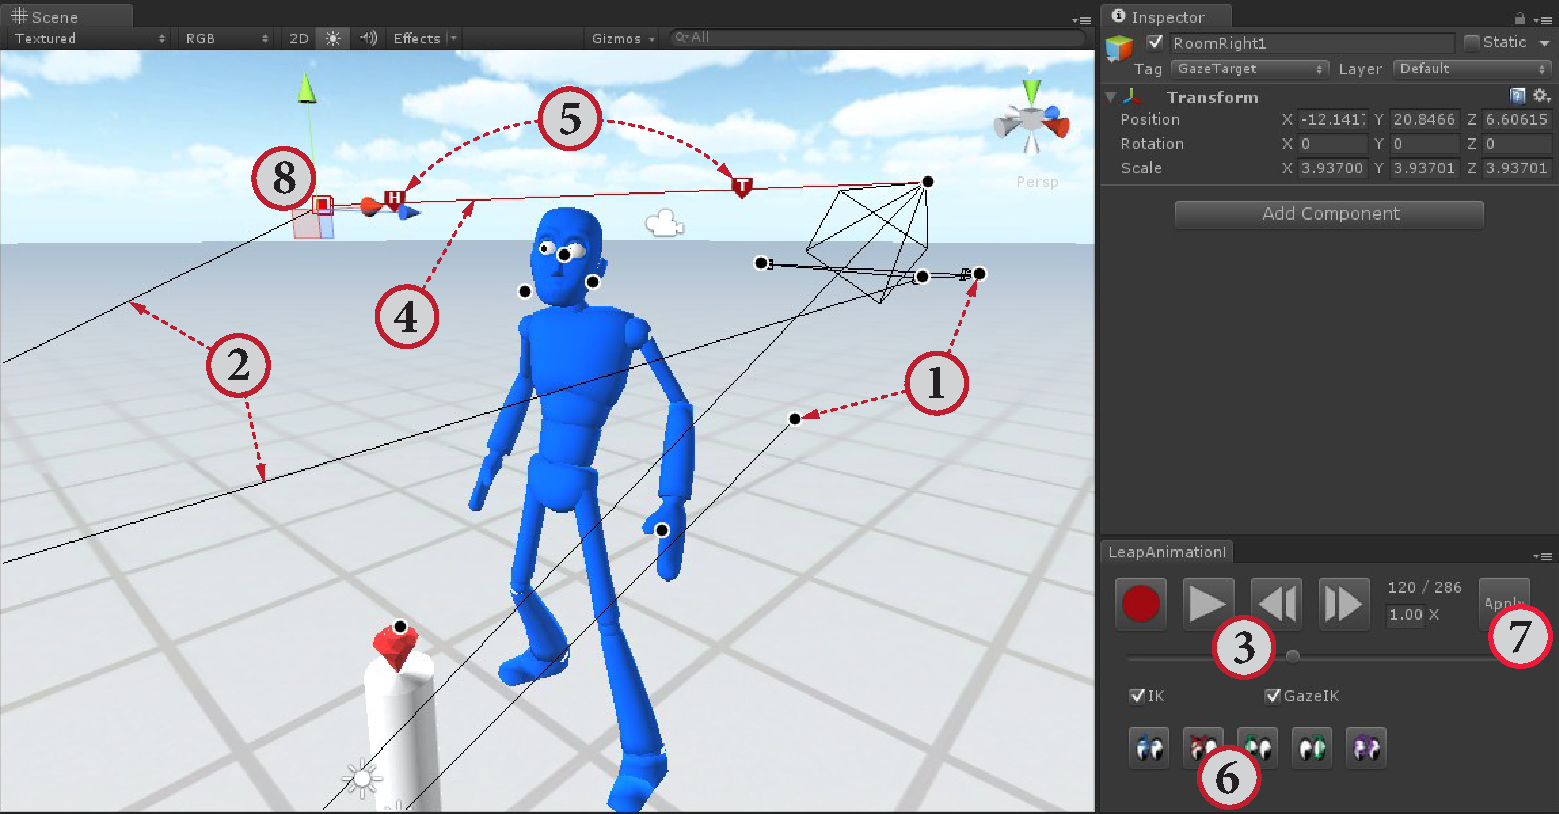
\includegraphics[width=0.9\textwidth]{gazeauthoring/Figures/GazeEditingTool.pdf}
\caption{Screenshot of the gaze editing interface: (1) gaze targets; (2) gaze sequence polyline; (3) timeline controls; (4) currently active gaze instance; (5) alignment parameter handles (H: head alignment; T: torso alignment); (6) gaze editing operations; (7) the ``Apply'' button, which synthesizes the edited animation; and (8) widget for moving a selected object or gaze target.}
\label{fig:GazeEditingTool}
\end{figure}

Gaze targets are implemented as tagged, dummy objects parented to scene objects and visually indicated in the scene view (Figure~\ref{fig:GazeEditingTool}, 8). For example, there is a gaze target object attached to the gem in Figure~\ref{fig:GazeEditingTool}. A large object can have multiple targets attached at different locations. Spatial editing of gaze can be done either by directly selecting and moving gaze target handles or by moving the scene objects to which they are attached. The latter method allows large-scale edits---all gaze shifts toward affected targets will adapt to their new locations.

\subsection{Results}
\label{sec:GazeEditingResults}

Our gaze authoring approach can produce believable results while requiring less labor and skill than traditional methods. An experienced animator must set many keyframes to add eye movements to a body motion, while our system can add an equivalent amount of animation automatically. Manually adding a new gaze shift to an existing gaze animation requires setting multiple keyframes on each of the eye, head, and torso joints, whereas our tool can accomplish the same result in a single operation. Much of the challenge in producing high-quality animation comes from getting the timing right---each keyframe needs to be placed with great care. Our tool greatly reduces this burden---the gaze shift model implements the kinematics of human gaze and automatically computes relative timings of eye, head, and torso movements that result in natural motion.

\begin{figure}
\centering
\includegraphics[width=1\textwidth]{gazeauthoring/Figures/Results.pdf}
\caption{Example motions generated using our system.}
\label{fig:GazeEditResults}
\end{figure}

Figure~\ref{fig:GazeEditResults} shows several examples of gaze animation created using our approach, excerpted from the supplemental video. Each example consists of two rows of images showing two versions of the same scene. Example 1 (WalkCones) demonstrates the effects of adding inferred eye movements to a walking motion. The eye movements make the character more lifelike and anticipate changes in trajectory. Example 2 (DrinkSoda) shows a story edit where a new character is introduced and the other two characters are made to gaze at her. In Example 3 (MakeSandwich), the character making a sandwich is made to look at the camera after adding each ingredient to increase the viewer's engagement. In Example 4 (WaitForBus), we prevented the character from checking his watch by removing the corresponding gaze instance and constraining his arm. Examples 5 and 6 show how we can use gaze edits to change the character's personality. Example 5 (ChatWithFriend) contrasts two versions of a first-person conversational scene, one where the character unsettlingly stares at the camera and another where it looks away uncomfortably. In Example 6 (HandShake), we made the character appear standoffish by having him look away during the handshake. 

\section{Evaluation}
\label{sec:GazeAuthoringEvaluation}
The goal of this work is to reduce the effort required to produce high-quality gaze animation modeling the gaze behavior as an automatically inferrable, easily editable sequence of gaze instances. %In this section, we present two evaluations we conducted to gauge our success: the first evaluation measured the authoring effort required to author and edit gaze using our approach in comparison with a traditional tool
We conducted a two-part evaluation of our approach. The first experiment assesses the amount of effort required to author gaze animations to confirm that our approach does save animator time and effort. The second experiment assesses the quality of the resulting animations, to ensure that sufficient quality is maintained.

\subsection{Authoring Effort}
\label{sec:GazeAuthoringEffortEvaluation}

We evaluated authoring effort in two ways. First, we investigated the effort required to add eye animation to a captured body motion without modifying the motion itself---something our tool can do automatically. We had two experienced animators add eye movements to seven scenes, originally captured for the gaze inference evaluation (Section ~\ref{sec:GazeAuthoringEffortEvaluation}), with cumulative length of 2:36 minutes. Both animators used Autodesk MotionBuilder, where they set up a simple eye animation rig, which they keyed to create the desired eye movements. We measured authoring effort using two metrics: (1) time taken and (2) number of keys set. We found that the animators required on average 25 minutes and 86 keys per minute of animation. By contrast, our system can synthesize an equivalent amount of eye animation automatically, requiring on average 90 seconds of computation per minute of animation.

Second, we assessed the effort required to edit gaze animation in a scene which already contained eye movements. An experienced animator was instructed to make the following edits: (1) introduce gaze aversion in a two-character interaction scene (HandShake), (2) remove gaze toward an object in an environment interaction scene (StealGem), (3) introduce gaze toward a new character in a multi-character interaction scene (DrinkSoda), and (4) introduce gaze toward the camera in an environment interaction scene (MakeSandwich). The edits in all the scenes involved changing not just eye movements, but also head and (in some cases) torso posture. To accomplish the edits, the animator used layering and keyframing features in MotionBuilder. Meanwhile, a novice animator authored the same edits using our gaze editing tool. As before, we measured time taken and number of operations required. For MotionBuilder, the latter is equivalent to the number of keys set, while for our tool, it refers to the editing operations discussed in Section~\ref{sec:GazeEditing}. The results, reported in Table~\ref{tab:GazeEditingEffortResults}, suggest equivalent edits may be achievable using our approach in 1/5 of the time and with 1/3 the number of operations required by traditional motion editing.
%
\begin{table}
\centering
\def\arraystretch{1.5}
\begin{tabular}{|l||l|l|l|l|}
\hline
\textbf{Scene} & \multicolumn{2}{l|}{\textbf{Traditional}} & \multicolumn{2}{l|}{\textbf{Our Approach}} \\
\cline{2-5}
& Time & \# keys & Time & \# ops  \\
\hline
HandShake & 10:40 & 19 & 3:11 & 8 \\
StealGem & 1:29 & 9 & 1:30 & 4 \\
DrinkSoda & 9:05 & 43 & 3:51 & 9 \\
MakeSandwich & 10:43 & 33 & 4:05 & 13 \\
\hline
\end{tabular}
\caption{Gaze editing effort: traditional vs. our approach.}
\label{tab:GazeEditingEffortResults}
\end{table}
%
\subsection{Animation Quality}
\label{sec:GazeAnimationQualityEvaluation}

To evaluate the effect of our gaze authoring approach on perceived quality of produced animation, we conducted a human subjects experiment. We compared our approach to other methods of gaze animation production: no eye animation, eye movements recorded using an eye tracker, and hand-authored gaze. We showed participants pairs of videos of a motion-captured character performing various actions and asked them to choose the one they thought had superior animation. The videos in each pair were identical in every way except the gaze animation method. Different methods corresponded to the following study conditions: (1) \emph{no gaze}, (2) \emph{recorded gaze} (using an eye tracker), (3) \emph{hand-authored gaze}, and (4) \emph{synthesized gaze} (our approach.)

\noindent\textbf{Hypotheses} -- We hypothesized the following: (1) \emph{Synthesized gaze} would be preferred over \emph{no gaze}. (2) \emph{Synthesized gaze} would be preferred over \emph{recorded gaze}. (3) \emph{Synthesized gaze} would be seen as equivalent to \emph{hand-authored gaze}. Hypothesis 2 is motivated by the consideration that raw eye-tracking data is noisy, non-trivial to map to an animated character, and often incorrect with respect to scene requirements. Hypothesis 3 reflects the expectation that our approach can synthesize gaze animation at a level of quality approaching hand-authoring.

\noindent\textbf{Design} -- The experiment involved three separate studies, each of which tested one of the hypotheses. Each study consisted of five task trials and followed a within-participants design, wherein the participants were asked to choose between videos in \emph{synthesized gaze} and one of the other conditions. Video pairs were presented to the participants in a randomized order.

\noindent\textbf{Stimuli} -- Experiment stimuli were $5 \times 4$ video clips (five scenes, each in four conditions) of a character animated using motion capture, 9 to 14 seconds in length. We created the \emph{no gaze} condition videos by extracting segments original scenes created for the gaze inference evaluation (Section~\ref{sec:GazeInferenceEvaluation}.) The scenes were: ChatWithFriend, MakeSandwich, StackBoxes, StealGem, WalkCones. The \emph{hand-authored gaze} condition was created by extracting those same segments from the scenes created for the authoring effort evaluation (Section~\ref{sec:GazeAuthoringEffortEvaluation}), while the \emph{synthesized gaze} condition was the result of applying our gaze inference to the segments. To create the \emph{recorded gaze} condition, we generated eye animations directly from eye tracking data.

\noindent\textbf{Measures} -- Our experiment had the following subjective measures: (1) perceived \emph{animator competence}, (2) \emph{realism}, and (3) \emph{communicative clarity}. The measures were implemented as binary-choice questions the participant answered on each task trial: (1) ``On which video did the animator do a better job?'' (2) ``In which video were the character\'s movements more realistic?'' (3) ``In which video did the character communicate more clearly what they were doing?''

\noindent\textbf{Participants} -- We conducted the experiment online using Amazon Mechanical Turk crowdsourcing service. We recruited 24 participants for each study---a total of 72 participants. The participants were paid at the rate of \$6/hour.
% TODO: Did you collect any demographics? I think people will at least expect gender breakdown.

\noindent\textbf{Results} -- Upon collecting our data, we conducted separate analyses for each study of the experiment. We aggregated all participants' binary answers across all the scenes and obtained, for each condition, the count of how many times it was chosen over its counterpart in each measure. Then we compared the counts using chi-square tests of goodness-of-fit. The results, shown in~\ref{fig:StudyResults}, were as follows.

\begin{figure}[t]
\centering
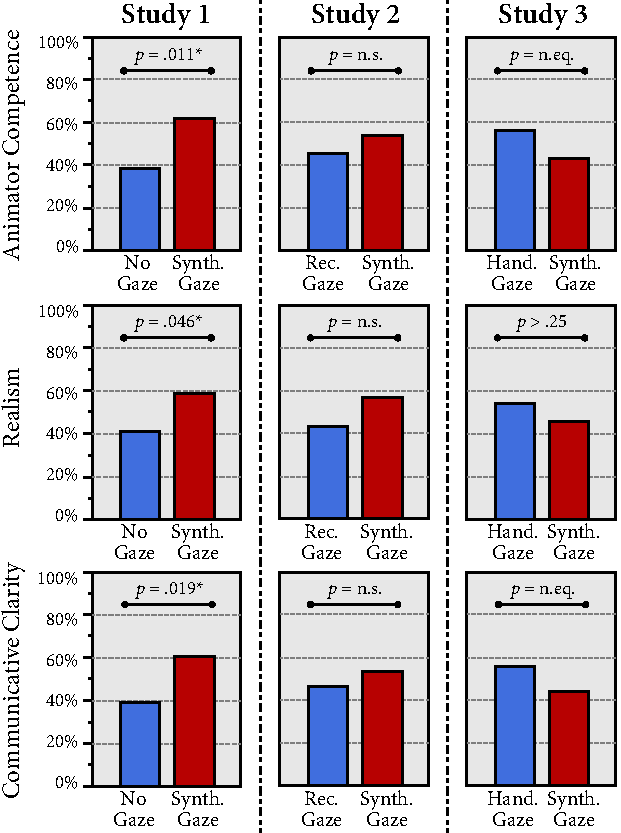
\includegraphics[width=0.48\textwidth]{Figures/StudyResults.pdf}
\caption{Results of the study comparing gaze animation produced using our approach (\emph{Synthesized Gaze}) to (1) no gaze animation, (2) gaze recorded using an eye tracker, and (3) hand-authored gaze. y-axis shows the percentage of trials in which one condition was chosen over the other.}
\label{fig:StudyResults}
\end{figure}

Our analysis of data from study one found a significant preference for \emph{synthesized gaze} over \emph{no gaze} on all measures: $\chi^2(1, 120) = 6.41, p = .011*$ (animator competence), $\chi^2(1, 120) = 3.99, p = .046*$ (realism), and $\chi^2(1, 120) = 5.54, p = .019*$ (communicative clarity.) These results constitute support for Hypothesis 1.

Data from the second study showed that \emph{synthesized gaze} was not significantly preferred over \emph{recorded gaze} in any of the measures: $\chi^2(1, 120) = 0.83, p = .362$ (animator competence), $\chi^2(1, 120) = 2.12, p = .145$ (realism), and $\chi^2(1, 120) = 0.53, p = .466$ (communicative clarity.) Therefore, we did not find support for Hypothesis 2.

In study three, chi-square test results were the following: $\chi^2(1, 120) = 2.12, p = .145$ (animator competence), $\chi^2(1, 120) = 0.83, p = .362$ (realism), and $\chi^2(1, 120) = 1.63, p = .202$ (communicative clarity.) While there was no significant difference in preference between \emph{synthesized gaze} and \emph{hand-authored gaze} on any of the measures, $p$-values also did not reach the suggested equivalence margin of $p \geq .50$~\cite{walker2011equivalence}, indicating lack of support for Hypothesis 3.

In a post-hoc exploratory analysis, we investigated the potential reasons for the lack of support for Hypothesis 2, as the findings contrasted our own observations. This analysis focused on how recorded and synthesized gaze differed across different scenarios in order to determine whether or not our approach had a differential effect on different scenes. We found that scene type had a significant effect on participants' choice of \emph{recorded gaze} in all measures (e.g., $\chi^2(4, 55) = 25.04, p < .0001^*$ for the ``animator competence'' measure). Further inspection showed that scenes with a close-up of the character benefited the most from our synthesized gaze approach, likely due to greater saliency of gaze cues. The differences between approaches were indiscernible in scenes where the character's eyes were small on the screen and other motion components dominated. An illustrative example is the ChatWithFriend scene, which was always chosen in \emph{synthesized gaze} condition over \emph{recorded gaze} in animator competence and realism measures, and 23 times out of 24 in communicative clarity.
%ChatWithFriend scene was always chosen in \emph{synthesized gaze} condition over \emph{recorded gaze} in animator competence and realism measures, and 23 times out of 24 in communicative clarity. We believe that is because ChatWithFriend scene showed a close-up of the character and placed emphasis on the gaze animation, which would have brought attention to high-frequency artifacts in recorded gaze and reduced the confounding effects of other animation components.
%In other scenes, where the eyes are small and other animation components dominate, it is unsurprising that we do not see a strong preference

Study results suggest that gaze animation is important for the perception of animation quality, and adding gaze animation using our approach leads to improvement in perceived animation quality. Benefits of gaze authoring may be more pronounced in scenes where gaze behavior is perceptually dominant. Finally, while we found no conclusive evidence that gaze authored by a trained expert was superior to the output of our method, we also did not find that they were equivalent in quality.
\begin{comment}
\subsection{Effectiveness of Editing}

HandShake
    1. How much was the green character focusing on the blue character?
        OG: $(M = 90.83\%, SD = 10.84)$
        NEG: $(M = 33.33\%, SD = 37.50)$
        $t(13) = -5.10, p = .0002*$
    2. How much was the green character focusing on the floor?
        OG: $(M = 21.67\%, SD = 31.57)$
        NEG: $(M = 82.50\%, SD = 21.79)$
        $t(20) = -5.49, p < .0001*$

MakeSandwich
    1. How much was the blue character focusing on the tabletop?
        OG: $(M = 62.50\%, SD = 27.01)$
        NEG: $(M = 54.17\%, SD = 22.75)$
        $t(21) = -0.81, p = .4227$
    2. How much was the blue character focusing on the camera?
        OG: $(M = 26.67\%, SD = 23.48)$
        NEG: $(M = 45.00\%, SD = 22.76)$
        $t(22) = 1.94, p = .0065$

PassSoda:
    1. How much was the blue character focusing on the green character?
        OG: $(M = 93.33\%, SD = 7.79)$
        NEG: $(M = 34.17\%, SD = 25.53)$
        $t(13) = -8.27, p < .0001*$
    2. How much was the blue character focusing on the pink character?
        OG: $(M = 5.00\%, SD = 7.98)$
        NEG: $(M = 70.83\%, SD = 22.75)$
        $t(14) = 9.46, p < .0001*$
        
StealGem
    1. How much was the blue character focusing on the red gem?
        OG: $(M = 79.17\%, SD = 25.75)$
        NEG: $(M = 50.00\%, SD = 41.78)$
        $t(18) = -2.06, p = .054$
    2. How much was the blue character focusing on the yellow gem?
        OG: $(M = 10.83\%, SD = 22.75)$
        NEG: $(M = 10.83\%, SD = 22.75)$
        $t(22) = 0, p = 1$

TODO: add figure StudyResults2
\end{comment}

\section{Discussion}
\label{sec:GazeAuthoringDiscussion}
The current chapter has proposed a novel approach for scalable authoring of gaze animation in non-interactive scenarios The approach is based on the idea of modeling the gaze behavior as a sequence of gaze instances, representing gaze shifts toward targets in the scene. We have shown how this representation can be automatically inferred from the body motion and scene geometry, producing an initial gaze animation that can be refined further through manual editing. We have also described a convenient gaze editing approach which takes advantage of the representation's two key properties: abstraction of gaze pose and timing details, and anchoring the gaze behavior in the scene via target handles. Finally, we have described a method for synthesizing plausible gaze animation from this representation and adding it to the original motion. As shown in the evaluations, the proposed approach can substantially reduce the labor and skill required to author gaze animation compared to traditional tools. Even a novice animator can endow characters with gaze at an acceptable level of quality, and it can also serve as a labor-saving tool for skilled animators by providing them with a first-guess animation they can edit further. In particular, the approach has potential applications in domains where quantity and speed of animation production are important considerations, such as television animation or animation of background and midground characters in film and games.

The gaze authoring approach could be extended in several ways.
For one, the accuracy and sensitivity of our gaze inference model could be further improved by replacing the current set of heuristics with models learned from recorded motion and gaze data.
In addition, the approach currently complements saliency-based methods for idle gaze, such as~\citep{peters2003bottomup}, but such models could be integrated with our own to refine the inference output.
Another property of the gaze inference model is that it produces a relatively conservative estimate of the gaze behavior. While it matches the body motion and scene, it does not have much expressiveness in the form of random saccades and idle gaze. Such aesthetic flourishes can mean the difference between adequate, yet uninteresting and truly lifelike animation, and professional animators spend much time getting them right. While probabilistic models for gaze behavior synthesis (e.g., ~\citep{lee2002eyes}) are no substitute for the skill of human artists, they can nonetheless be integrated with our gaze authoring approach to obtain a richer, more lifelike gaze behavior without the need for manual intervention.
Finally, the purpose of the gaze authoring approach is adding editable gaze animation to non-interactive scenarios. However, the gaze inference model could be adapted to operate on interactive inputs, allowing its use for predicting user attention and intent in virtual reality and other interactive contexts.

The current implementation of the system in Unity serves as an adequate proof of concept, but its utility to artists would be increased by integration with a 3D animation software such as MotionBuilder or Maya. Furthermore, the system uses a feed-forward gaze shift controller for motion synthesis as well as a gaze shift parametrization that defines head and torso alignments relative to the current pose rather than the target location. Due to these design decisions, the entire motion needs to be synthesized from start to end to obtain the final editing result. To make the system more immediate, alternative motion synthesis methods might need to be explored. While the complexity of the gaze shift model (Chapter~\ref{cha:GazeShiftModel}) precludes a closed-form formulation, a simplified version of the model could be designed that would allow exact pose computation on a per-frame basis.


\chapterstyle{deposit}
\pagestyle{deposit}

\chapter{Discussion}
\label{cha:Discussion}

Human attending behaviors involve movements of the eyes, head, and body, and they play a number of important communicative roles in human perception, social interaction, and cognition. The communicative effectiveness of these behaviors comes from their remarkable kinematic variability: quick eye saccades, eye-head shifts, upper-body and whole-body reorientations are movements with similar kinematic profiles, yet they appear very different and yield very different effects in communication. Producing convincing animation of such movements on virtual characters is a challenging problem, both in interactive and non-interactive contexts.
In interactive contexts, we require methods that can synthesize the highly varied gaze movements in a controllable fashion. These movements then need to be utilized as primitives for building more complex gaze behaviors that trigger specific effects in people observing or interacting with the character.
Moreover, since virtual characters can differ morphologically from realistic humans, we require methods that can adapt the kinematics of humanlike gaze movements to account for morphological differences.
In non-interactive, authoring contexts, the challenge also lies in animator skill and effort required to author high-quality gaze movements. This challenge is compounded by the poor scalability of manual authoring with respect to scenario complexity and scene changes. Traditional animation authoring methods, such as keyframing and IK, do not ensure good scalability on any of those dimensions.

This works posits that the problem of creating effective attending behaviors on animated characters can be solved more easily by modeling those behaviors as sequences of \emph{directed gaze shifts}. To prove this thesis, we contributed several methods for synthesis of directed gaze shifts, a new conversational gaze mechanism for virtual agents, a workflow and tool for authoring directed gaze animation, and a set of empirical insights about directed gaze as a model for interactive and non-interactive gaze behaviors. An overview of the contributions is given in Table~\ref{tab:Contributions}.

\begin{table}
\small
\centering
\def\arraystretch{1.5}
\begin{tabularx}{\textwidth}{lp{10.8cm}r}
\hline
\textbf{Category} & \textbf{Contribution} & \textbf{Chapter} \\
\hline
\multirow{5}{*}{Technical} & Gaze shift synthesis model & \ref{cha:GazeShiftModel} \\
& Stylized gaze & \ref{cha:StylizedGaze} \\
& Performative gaze & \ref{cha:StylizedGaze} \\
& Gaze inference from body motion & \ref{cha:GazeAuthoring} \\
& Gaze motion layering & \ref{cha:GazeAuthoring} \\
\hdashline
\multirow{3}{*}{Design} & Gaze editing approach & \ref{cha:GazeAuthoring} \\
& Gaze authoring workflow & \ref{cha:GazeAuthoring} \\
& Nonverbal signals of conversational footing & \ref{cha:GazeFooting} \\
\hdashline
\multirow{10}{*}{Design} & Gaze shift model synthesizes plausible, communicatively accurate gaze shifts & \ref{cha:GazeShiftModel} \\
& Gaze shifts with more torso reorientation are stronger attention cues & \ref{cha:GazeShiftModel} \\
& Virtual agents can use gaze and spatial orientation to manage footing & \ref{cha:GazeFooting} \\
& Nonverbal footing signals are effective only in immersive VR & \ref{cha:GazeFooting} \\
& Gaze adaptation to stylized characters reduces animation artifacts & \ref{cha:StylizedGaze} \\
& Stylized and performative gaze adaptations do not impair communicative accuracy or plausibility & \ref{cha:StylizedGaze} \\
& Human actor's gaze can be reconstructed from their body motion and scene layout & \ref{cha:GazeAuthoring} \\
& Gaze authoring approach allows novices to create and edit gaze animation with less effort & \ref{cha:GazeAuthoring} \\
& Animation obtained from the gaze authoring approach looks plausible & \ref{cha:GazeAuthoring} \\
& Edited gaze animation communicates a different attention distribution & \ref{cha:GazeAuthoring} \\
\hline
\end{tabularx}
\caption{Research contributions from this dissertation.}
\label{tab:Contributions}
\end{table}

In the remainder of this chapter, I discuss potential applications of the methods and findings contributed in this work, as well as their limitations and possible directions for future research.

\section{Applications}

Gaze synthesis and authoring methods introduced in this dissertation can be applied to animated characters in a wide range of applications. The gaze shift synthesis model (Chapter~\ref{cha:GazeShiftModel}) is designed primarily for interactive applications, such as non-player characters in games, player avatars, and embodied conversational agents, but we have also integrated it into an animation authoring workflow (Chapter~\ref{cha:GazeAuthoring}).
With its parametric control over head, torso, and whole-body orientation, the gaze shift model is also uniquely applicable to synthesis of nuanced attending behaviors that occur in multiparty interactions. One example are the nonverbal footing signals introduced in Chapter~\ref{cha:GazeFooting}, which can be utilized by virtual agents engaging in multiparty interactions with users in order to influence users' conversational contributions. Such behaviors may become an essential component in social experiences built for virtual and mixed reality media, where users are more sensitive to the spatial arrangement and nonverbal cues of interaction participants.

Stylized gaze methods (Chapter~\ref{cha:StylizedGaze}) have the potential to expand the range of character designs that can be animated by existing gaze models. There are many reasons why authors might want to employ characters with stylized features: such characters might be seen as more appealing than realistic, humanlike characters; they might connect better with the target demographic (e.g., children); their design might be exaggerated to emphasize specific personality traits, etc. While online motion retargeting to such characters is still an open problem, the methods introduced in the current work allow transfer of a specific subset of humanlike motion---directed gaze.

Finally, one application domain that has hitherto received almost no attention in computer animation research on gaze has been animation authoring. Even though much of the facial and body animation seen in today's computer-generated films is captured, eye movements still tend to be hand-authored from scratch. Moreover, editing the characters' gaze animation is still accomplished using labor- and skill-intensive tools. Chapter~\ref{cha:GazeAuthoring} introduces an authoring approach designed to assist in the production of gaze animation in non-interactive contexts, such as game cutscenes, television, and film animation. In addition to the ability to automatically add plausible eye animation to captured scenes, the approach enables convenient authoring and editing of gaze animation by novices. As such, it can serve as a labor-saving tool for experienced animators to give them a starting point for gaze animation editing, but it can also enable novices to author gaze animation at a scale and level of quality that would be beyond their reach using traditional methods.

\section{Limitations and Future Directions}

\subsection{Increasing Gaze Expressiveness}

Major advantages of directed gaze as a model of humanlike attending behaviors are its simple parametrization and uniform nature---the entire behavior is modeled as a sequence of gaze shifts parametrized by timing, target, and head and torso alignments. These advantages come with a downside---the resulting behavior is relatively predictable and lacks expressive variation in eye, head, and body movements. The lack of variation in head and body movements is less of a problem in gaze authoring (Chapter~\ref{cha:GazeAuthoring}), where much of the expressiveness is already encoded in the body motion, but it becomes more noticeable when animating virtual agents, which can appear static and robot-like as a result.
On the other hand, the often sparse and predictable eye movements yielded by our gaze inference model, while plausible, do not approach the rich expressiveness seen in professionally animated characters, where ``each new thought triggers an eye movement''~\citep{maestri2001digital}.

Directed gaze is not an all-encompassing model of human gaze movements. For example, it excludes gaze movements such as eye blinks, smooth pursuit and pupil dilation. Animators may wish to incorporate such movements to make their characters look more expressive. While some of these movements are simulated in prior work (e.g., smooth pursuit~\citep{yeo2012eyecatch}), integrating them into our models would be far from straightforward. For example, to support smooth pursuit in our gaze authoring approach would require not just new synthesis methods, but also new movement parametrizations and a gaze inference model that can automatically detect gaze at moving objects.

To improve the expressiveness of the gaze behaviors generated by our models, we enrich them with probabilistically generated eye blinks and saccades added in a post-process. We generate the blinks as described by~\citet{peters2010animating}, while for saccadic gaze we use the Eyes Alive model~\citep{lee2002eyes}. These behaviors make the character look more lively, but they do not improve its communicative expressiveness, as they are generated without regard for context or high-level state. Saccades in humans reflect changes in cognitive state and speech content, while blinks correlate with emotion, personality, and alertness. Our models do not capture these high-level contingencies; they introduce saccades and blinks based only on the low-level gaze shift sequence. As I discuss further below, more sophisticated modeling may be required to capture the communicative variety of real human gaze.

\subsection{Building Better Gaze Models}

The focus of this dissertation is on enabling the use of directed gaze shifts as building blocks of more sophisticated gaze behaviors and as a primitive for motion editing. Automatic production of communicatively effective gaze patterns is the task of high-level gaze models. Although such models are not the primary focus of the current work, two are nonetheless contributed: a gaze model for virtual agents engaging in multiparty interactions (Chapter~\ref{cha:GazeFooting}) and a model for gaze behavior inference from a captured body motion and scene (Chapter~\ref{cha:GazeAuthoring}). Future work can explore building other models that use directed gaze shifts as units of behavior. Example use cases where directed gaze is a good abstraction are various conversational mechanisms (e.g., configuring the conversational formation, turn-taking, intimacy regulation), attention in visually-guided tasks, attending behaviors in crowds, and idle gaze.

Many prior gaze models---including the ones in this dissertation---generate gaze sequences using relatively simple stochastic-heuristic methods. These methods do not always adequately capture the complexity of human attending behaviors and may give rise to gaze behaviors that look implausible or communicate the wrong thing. Part of the problem is that humans do not produce gaze cues in isolation, but in coordination with other aspects of behavior, such as speech, facial expressions, hand gestures, proxemics, locomotion, etc. In order to look plausible and communicate effectively, an animated character must display gaze cues that match other aspects of its visible and audible behavior. The multitude of behavioral contingencies are not adequately modeled by heuristic rules and low-order statistics utilized in many current models.

Future work should investigate probabilistic models learned from time-series data for gaze behavior synthesis. In particular, Markov Decision Processes (MDP) and reinforcement learning may be suitable approaches when the character's high-level state is fully or partially known (observable). This is usually the case with autonomous agents, whose attention, communicative intent, and cognitive state are computationally modeled. Models such as Hidden Markov Models (HMMs) and Dynamic Bayesian Networks (DBN) are appropriate for cases where the high-level state is unknown, such as when the character is animated using motion capture data or controlled by a human player using various tracking devices. Since such models can capture temporal contingencies among different behavioral modalities, as well as their relationships to the current communicative context, I hypothesize they will enable synthesis of more plausible and communicatively effective gaze behaviors.

\subsection{Gaze Model Generality}

This dissertation has introduced directed gaze as model of attending behaviors that generalizes well across different contexts. We have used directed gaze shifts as building blocks of joint attention signals, multiparty-conversational gaze behaviors, and an abstraction for gaze authoring. However, there are many factors within those contexts that our models do not account for, which should affect the gaze patterns produced by the models. One major factor is \emph{user gender}. There are significant cross-gender differences in gaze perception, which we also detected in our own studies, e.g., in Chapter~\ref{cha:GazeFooting}. Other user-characteristic factors include \emph{personality}---e.g., extroverts are known to engage in significantly more eye contact than introverts~\citep{rutter1972visual}---and \emph{culture}---e.g., multiple studies suggest that people from Western cultures initiate more eye contact than those from Eastern cultures~\citep{mccarthy2006cultural,mccarthy2008gaze}. Furthermore, our models do not account for scenario variations. For example, the gaze model in Chapter~\ref{cha:GazeFooting} is not a universal model for signalling footing in multiparty interactions. It is based on data from scenarios involving a lot of verbal interaction and mutual gaze~\citep{mutlu2012conversational} and it may not generalize to scenarios involving (for example) more referential gaze and object manipulation. Finally, attributes of the virtual character, such as gender, realism, desired personality, and even species, may also affect how people respond to its gaze. While we have introduced methods that account for variations in character design, we did not extensively evaluate how these variations might modify the social and cognitive effects of gaze, even though prior research indicates that effects of embodiment on user behavior may be substantial~\citep{parise1996my}.

To optimize the effects of the character's gaze behavior on the current user, high-level gaze models should incorporate the user's attributes, scenario type, and character attributes as parameters, and they should adapt the output behavior based on their values. Since these effects are often subtle, accounting for them may require extensive data collection from an appropriately chosen participant pool. However, the benefits could be significant. For example, the agent in Chapter~\ref{cha:GazeFooting} could decrease the amount of mutual gaze with female users to avoid making them uncomfortable, while the gaze inference model (Chapter~\ref{cha:GazeAuthoring}) could make a character appear more introverted by decreasing the amount of gaze toward other characters.
% TODO: discuss other limitations:
% - Simplicity of model tasks/scenarios in our evaluations

\subsection{Adapting Gaze to User Behavior}

Directed gaze is an effective model for realizing several conversational gaze behaviors. Chapter~\ref{cha:GazeFooting} describes a set of gaze and spatial reorientation cues for virtual agents allowing them to manage conversational footing in interactions with one or more users. While still preliminary in many ways, this work motivates the need for virtual agent systems that can effectively engage with users in multiparty interactions and exposes a number of research challenges. To be effective at managing multiparty interactions, agent systems need to use the information about the users' engagement intents, attention, and environment layout, to make decisions about the agent's positioning, reorientation, and gaze patterns, such that desired communicative goals are achieved. Possible goals include: (1) establish and reconfigure the conversational formation to make optimal use of available space; (2) use appropriate gaze behaviors and proxemics to maximize users' comfort level; (3) manage conversational footing to optimize users' level of participation and sustain their interest; (4) manage turn-taking to avoid ambiguities and breakdowns in communication.

A particularly salient lesson from our project is one of the need to make inferences about users' intents in order to avoid communication failures and keep them engaged. Some of the most egregious mistakes committed by the agent involved cutting off the participant due to an erroneous belief that they were finished with their utterance. This could have been avoided if the system possessed a more comprehensive model of turn-taking behaviors, including the ability to sense the participant's floor-holding cues such as averted gaze. Similarly, the experience of female participants may have been negatively affected when the agent engaged in too much mutual gaze. To avoid such effects, embodied agent systems should be more sensitive to users' intimacy-regulating signals---gaze aversions and interpersonal distance---and adjust their own behavior in response. Future work will need to take better advantage of the sensing capabilities afforded by modern VR devices---e.g., head and eye tracking---to characterize user behavior and make appropriate decisions about the agent's behavior based on those inferences.

\subsection{Scalable Authoring of Attending Behaviors}

Chapter~\ref{cha:GazeAuthoring} of this dissertation has introduced the first animation authoring approach designed specifically for gaze, built around directed gaze as the underlying model. While the approach succeeds in its goal of reducing authoring effort while producing motion at an acceptable level of quality, it can still be significantly improved upon. First, the computational efficiency of gaze motion synthesis is still insufficient for truly interactive editing, due to the alignment parametrization and feed-forward design of the gaze shift model, which requires the entire motion to be resynthesized to see the exact editing result. Second, the current authoring approach is not yet comprehensive enough to allow universal editing of characters' attending behaviors, as it lacks support for whole-body orientation. Editing whole-body orientation as well as eye gaze is challenging since it requires editing the entire underlying body motion, which involves root movements and complex patterns of end-effector constraints. Existing methods such as motion path editing~\citep{gleicher2001path} may provide a good starting point for implementing such features.

With improved computational efficiency and ability to edit whole-body movements, the approach could be used for editing attending behaviors of groups and crowds of characters in a scalable manner. Attending behaviors in such contexts are more complex than simple gaze and spatial orientation shifts. Groups of interacting people arrange themselves into conversational formations~\citep{kendon2010spacing}, they maintain mutual gaze and interpersonal distance appropriate to their situation and intimacy level~\citep{argyle1965eyecontact}, and their gaze patterns reflect a number of joint perceptual, attentional, and social-cognitive processes. To synthesize such behaviors automatically and enable their convenient editing entails a slew of research challenges. These include computational modeling of the principles that govern human social behavior, designing editing handles that map intuitively to parameters of large-scale social interactions, and developing new motion synthesis and editing methods that can handle complex, multi-character, spatial and temporal constraints. The methods and designs presented in the current work represent but the first steps toward a more comprehensive editing approach. 

%% etc, etc.

%% Do you have appendices?  If so, add them here, just like chapters.
% \begin{appendices}
% \include{backmatter/appendix1}
% \end{appendices}

%% Are you a big nerd with a colophon?  Add it here.
%\begin{colophon}
%\svnidlong{$LastChangedBy$}{$LastChangedRevision$}{$LastChangedDate$}{$HeadURL: http://freevariable.com/dissertation/trunk/frontmatter.tex $}
\vcinfo{}

This template uses Gyre Pagella by default.  (I used Arno Pro in my dissertation.)

Feel free to give me a shout-out in your colophon or acks if this template is useful for you.  Good luck!

%\end{colophon}

%% McBride is a very nice style (some version is included in this distribution)
\bibliographystyle{mcbride}
\bibliography{refs}

%% Want an index?  Neither did I.
%\printindex

\end{document}
